\bookpart{图与信号}{Graphs and Signals}
\label{part:discrete-mathematics-and-graph-theory}
\label{part:graphs-and-signals}

\BookPartGuide{%
本部分研究两类带结构的数据：图用顶点和连接表示对象之间的关系，信号则记录
各个时间或位置上的数值。二者都要回答怎样表示、怎样计算以及变换后保留
了什么信息，图的连接说明哪些对象相连，信号的数值说明各位置记录了什么。

第8章“信号的表示与计算”研究信号的基、频率表示、卷积与相关、快速变换、采样和
恢复，并明确有限记录、离散实现与连续模型之间的边界。第9章“图的表示与计算”
建立图、路径、连通、分离和结构分解，讨论遍历、最短路、生成树、匹配、割、谱方法
及图上的传播。

图章关注关系怎样限制可达路径和组合选择，信号章关注数值怎样分解、变换与重构。
图上的函数把两类对象连接起来：图决定允许比较哪些位置，函数值承载要传播或滤波的
信息。}

\chapter{信号的表示与计算}
\label{chap:signal-analysis}

一段传感器记录既可以按时间逐项读取，也可以分解成不同频率的波动。
两种读法描述同一条信号，却适合回答不同问题：变化发生在何处，哪些振荡占主导，
一个局部滤波怎样作用，以及只保留部分样本后还能知道什么。这里需要分清三件事：
换一组完整坐标不一定丢失信息，滤波会改变信号，而采样会改变可用的观测。
计算某种表示很快，也不能代替对信息是否保留的判断。

本章沿用两个有限记录
\begin{equation}
  \bm x=(1,2,1),\qquad \bm h=(1,-1)
  \label{eq:signal-analysis-running-example}
\end{equation}
说明位置、边界、卷积与相关；需要非对称波形或连续时间时另行明确输入。
信号先作为带索引的函数出现，内积和范数给出共同的比较口径。
在此基础上，脉冲、复指数与多项式提供不同表示，输入输出映射说明如何改变信号，
采样条件则决定哪些区别仍能从观测中恢复。一般函数空间与线性坐标的背景可回查
第~\ref{chap:functional-analysis-and-approximation}章和第~\ref{chap:linear-algebra}章。
本章着重利用规则时间或位置索引；下一章再把位置之间的关系推广为一般图，
比较规则平移与图上传播的区别。至于怎样用内部状态产生输入输出响应，留给
第~\ref{chap:dynamical-systems-and-state-estimation}章。

\section{信号的对象与结构}
\label{sec:signal-objects-structure}

“三个数”还不是完整的信号说明。它们可能是三个时刻的温度，也可能是同一时刻
三个传感器的读数；数组首尾可能互不相连，也可能代表一个周期。
在比较大小或选择表示以前，需要先确定索引、取值和边界分别表示什么。

\subsection{信号的索引与取值}

\subsubsection{连续、离散与有限信号}

信号（signal）是定义在某个时间或位置索引集上的函数，函数值记录对应位置的量。
连续时间信号写成$x(t)$，离散时间信号写成$x[k]$；这里的“连续”描述索引，
不要求函数值随时间连续。例如发生突跳的开关读数仍是连续时间信号。

\begin{definition}[信号的索引类型]
  \label{def:signal-index-types}
  连续时间标量信号是$x:I\to\mathbb F$，其中$I\subseteq\mathbb R$为时间区间，
  $\mathbb F$取$\mathbb R$或$\mathbb C$。
  \term{离散时间信号}（discrete-time signal）是$x:\mathbb Z\to\mathbb F$，
  或定义在明确指定的整数子集上。长度$N$的有限信号是
  $x:\{0,\ldots,N-1\}\to\mathbb F$，可按位置写成$\bm x\in\mathbb F^N$。
\end{definition}

数组下标只是位置编号。若第$k$项来自时刻$t_0+kT_s$，还要给出起点$t_0$及间隔
$T_s$，才能把“每两项一次振荡”换算成物理频率。不等间隔观测则需要显式保存每个
时间戳，不能直接套用均匀采样公式。二维图像以两个整数坐标标位置，规则网格上的
运算可以相应推广到$\mathbb Z^d$，但一般图节点的编号不自带这种平移结构。

有序信号与无序样本集合也不同。$(1,2,1)$和$(1,1,2)$有同样的取值及重数，
相邻变化却不同，因此局部差分或模板比较可以区分它们。
随机信号则是在概率空间上给每个索引配一个随机变量；固定一次随机结果$\omega_0$
后，$k\mapsto X_k(\omega_0)$成为一条确定路径。对这条路径求频谱与对随机信号求
期望是不同操作，一次观察不自动给出总体规律。本章先研究给定的确定信号，
随机变量、过程及期望在第~\ref{chap:random-variables}章建立后再用于随机信号。

复数值常用来同时记录两个实分量或表示振荡的幅度与相位。
记$\mathrm i^2=-1$，对$z=a+\mathrm ib$有
$\overline z=a-\mathrm ib$、$|z|^2=z\overline z=a^2+b^2$。
这里的\term{复共轭}（complex conjugate）只改变虚部符号，不是时间反转；
后文内积中的共轭正是为了使自内积得到非负的大小。

\subsubsection{单通道与多通道信号}

立体声在同一时刻有左右两路读数。将两路首尾接起来会把通道差别误当成时间先后，
因此需要分别记录这两种索引。
\begin{definition}[标量信号与向量值信号]
  \label{def:signal-multichannel}
  单通道信号在每个位置取一个标量值。$d$通道信号在每个位置取向量值
  $\bm x[k]=(x_1[k],\ldots,x_d[k])^\top\in\mathbb F^d$；
  连续时间时相应写作$\bm x(t)$。
  $N$个位置的记录可写为$\bm X\in\mathbb F^{N\times d}$，
  约定$\bm X_{k+1,c}=x_c[k]$，其中$k=0,\ldots,N-1$、$c=1,\ldots,d$。
\end{definition}

时间轴长度为$N$，通道数为$d$，两者不互换。比如
\begin{equation}
  \bm X=
  \begin{bmatrix}1&0\\2&1\\1&2\end{bmatrix}
  \label{eq:signal-multichannel-record}
\end{equation}
有三个时刻、两个通道；第二行$(2,1)$是同一时刻的联合读数。
把两个传感器放在同一个向量里，隐含它们已经按同一时间基准对齐；若第二通道延迟
一个采样间隔，应先保留这一偏移，不能把不同时刻的值当作同时观测。
多通道既不意味着通道独立，也不意味着必须逐通道处理：
可以对每一列分别滤波，也可以在每个时刻以矩阵混合多个通道。
后者的输入输出维度及时间作用将在第~\ref{sec:signal-input-output-maps}节明确区分。

\subsection{信号的周期与边界}

\subsubsection{周期信号与非周期信号}

重复观察到相似波形不等于已经证明周期性。周期要求整个定义域上的精确重复，
还要求每次平移都留在允许的索引内。
\begin{definition}[周期及基本周期]
  \label{def:signal-period}
  定义在$\mathbb R$上的信号$x$若存在$T>0$使$x(t+T)=x(t)$对所有$t$成立，
  则称其为周期信号，$T$为一个周期。
  定义在$\mathbb Z$上的信号若存在正整数$N$使$x[k+N]=x[k]$对所有整数$k$成立，
  则称其为周期序列。若正周期中存在最小者，才称其为基本周期。
  没有正周期的信号称为非周期信号。
\end{definition}

在按几乎处处相等识别函数的空间中，周期等式也按几乎处处理解。
常数连续信号的每个正实数都是周期，却没有最小正周期；
离散周期的候选是正整数，非空时一定有最小者。
连续复指数$e^{\mathrm i\Omega t}$在$\Omega\neq0$时有基本周期
$2\pi/|\Omega|$；离散复指数$e^{\mathrm i\omega k}$则要求
$e^{\mathrm i\omega N}=1$，即$\omega/(2\pi)$为有理数，才有整数周期。
所以连续振荡取样后是否周期还取决于取样间隔与振荡周期的比例。

多通道周期要求所有通道具有一个共同周期。例如
\[
  \bm x(t)=\begin{pmatrix}\cos t\\\cos(\sqrt2\,t)\end{pmatrix}
\]
的每一分量都周期，
但共同周期必须同时满足$T=2\pi m$和$\sqrt2 T=2\pi n$，
其中$m,n$为整数；无理数$\sqrt2$使正$T$不可能存在。
离散的有限多个周期通道则可取各整数周期的最小公倍数作为共同周期。

还应区分三个对象：物理信号本来周期，有限数组被人为周期延拓，
以及变换所得频谱以某个频率间隔重复。DFT可以给任意有限数组配置循环索引，
不要求记录前后的真实过程恰好重复；DTFT的频率周期来自整数时间索引，
也不要求原序列周期。这些区别会决定后文“回绕”发生在时间轴还是频率轴。

\subsubsection{有限支撑与边界延拓}

有限记录只说明观测范围。为了计算跨过首尾的运算，还必须说明区间外采用什么值。
离散信号的支撑是$\{k:x[k]\neq0\}$；只有有限个非零位置时称为有限支撑。
连续信号通常以非零集合的闭包定义支撑，$L^p$类中使用忽略零测差别的本质支撑。
连续时间的有限支撑在此指支撑包含于某个有界区间，不是只有有限个非零点。

对$x[0],\ldots,x[N-1]$，零延拓令区间外的值为零；
周期延拓令$x[k]=x[k\bmod N]$；反射延拓则把边界附近的值镜像放到区间外。
反射有不同端点约定。例如不重复端点且$N\geq2$时，
$x[-1]=x[1]$、$x[N]=x[N-2]$，再以$2(N-1)$为周期延续；
若重复端点，就有$x[-1]=x[0]$、$x[N]=x[N-1]$，得到另一个延拓。
两种方式都可能合理，但不是同一个输入。

贯穿例$(1,2,1)$零延拓后，左边相邻值为$0$；周期延拓时为$1$；
不重复端点的反射延拓时为$2$。在位置$0$计算当前值减前值，三者分别得到
$1,0,-1$。这个差别出现在运算之前，不能由之后采用哪种快速算法来决定。

输出裁剪又是另一项选择：先按给定延拓计算输出，再只保留指定位置。
裁去首尾不等于改变输入延拓，保持输出长度也不能唯一决定左右怎样补值。
周期索引上的运算只在一个周期内计数；若把两条周期延拓序列直接在整轴上无穷求和，
同一个贡献会重复无穷次。这一边界将在循环卷积的定义中保留。

\subsection{信号的比较与大小}

\subsubsection{基于内积的信号比较}

判断两个记录是否接近，需要决定哪些位置和通道参与比较。
第~\ref{chap:functional-analysis-and-approximation}章使用实内积；
本章扩展到复信号时采用第一变量线性、第二变量取共轭的约定。
它与第~\ref{sec:linear-algebra-length-angle-distance}节的复坐标约定互为共轭，
实信号时两者相同；范数与正交性不变，读取展开系数时却要相应调整内积的顺序。
对有限记录、平方可和序列与平方可积函数，分别有
\begin{equation}
  \begin{aligned}
    \langle x,z\rangle_N&=\sum_{k=0}^{N-1}x[k]\overline{z[k]},\\
    \langle x,z\rangle_{\ell_2}&=\sum_{k\in\mathbb Z}x[k]\overline{z[k]},\\
    \langle x,z\rangle_{L^2}&=\int_{\mathbb R}x(t)\overline{z(t)}\,\mathrm dt.
  \end{aligned}
  \label{eq:signal-inner-products}
\end{equation}
后两式的乘积由Cauchy--Schwarz不等式保证绝对可和或绝对可积。
内积为零表示在当前比较口径下正交，诱导距离为$\|x-z\|_2$。
非零信号的归一化比较量
$\rho(x,z)=\langle x,z\rangle/(\|x\|_2\|z\|_2)$满足$|\rho|\leq1$；
实信号时这是夹角余弦，复信号时它一般是复数，包含相对相位。
零信号没有这种归一化相似性，不能直接除以零。

例如$x=(1,2,1)$、$z=(1,0,-1)$满足$\langle x,z\rangle=0$，
但两者在位置$0$都有非零值。正交描述汇总贡献抵消，不要求支撑互不相交。
若把$x$变成$2x$，归一化相似性仍为$1$，距离却为$\|x\|_2$；
这说明方向相同与数值接近是两个判断。

多通道内积同时汇总位置与通道：
\[
  \langle\bm x,\bm z\rangle
  =\sum_k\sum_{c=1}^d x_c[k]\overline{z_c[k]}.
\]
如果不同传感器的单位或重要性不同，可明确选正权重$w_c$，
把每项乘以$w_c$。更一般地，Hermitian正定矩阵$\bm W$给出
$\sum_k\bm z[k]^*\bm W\bm x[k]$，其中$*$表示共轭转置。
正定性使非零信号的自内积为正；仅半正定时某些非零通道组合可能被忽略。
改变权重可能改变正交关系及相似性排序，不能把它当作不影响结论的单位装饰。

\subsubsection{基于范数的信号大小}

峰值关心某一时刻是否过大，绝对累计关心全部幅值的总量，平方累计更强调大幅值。
对离散标量信号，相应范数是
\[
  \|x\|_\infty=\sup_k|x[k]|,\qquad
  \|x\|_1=\sum_k|x[k]|,\qquad
  \|x\|_2=\left(\sum_k|x[k]|^2\right)^{1/2}.
\]
在有限记录上求和只取记录范围；整轴上则要求相应总和有限。
记$\ell_1(\mathbb Z)$为绝对可和序列空间，$\ell_2(\mathbb Z)$为平方可和序列空间。
例如$x[k]=(k+1)^{-1}$在$k\geq0$时取此值、在$k<0$时取零，
属于$\ell_2$却不属于$\ell_1$。所以可以定义能量的信号未必能直接使用
绝对收敛的变换或卷积论证。

连续情形将和换成积分，得到$L^1$与$L^2$范数；$L^\infty$采用
$\operatorname*{ess\,sup}_t|x(t)|$，即忽略零测异常点后的最小本质上界。
这不同于最大值：函数可能只趋近其上界而未取到，也可能在单个点被赋任意大值，
但代表同一个$L^\infty$元素。真实采样要读取点值，届时必须另行确定代表元。

对贯穿有限记录，$\|x\|_\infty=2$、$\|x\|_1=4$、$\|x\|_2=\sqrt6$。
重排位置不改变这三个数，却可以改变局部波形；范数不是完整的形状描述。
多通道的二范数可按
$\|\bm x\|_2^2=\sum_k\|\bm x[k]\|_2^2$定义，
若使用前述$\bm W$，则改为$\sum_k\bm x[k]^*\bm W\bm x[k]$。
比较前须固定通道度量，不能把不同单位的读数无说明地相加。

\subsubsection{有限能量与平均功率}

持续振荡的幅值可以有界，但持续时间无限，平方累计仍会发散。
这时需要区分累计了多少与每单位时间平均有多少。
\begin{definition}[信号能量与平均功率]
  \label{def:signal-energy-power}
  离散及连续信号的能量分别为
  \[
    E_x=\sum_{k\in\mathbb Z}|x[k]|^2,\qquad
    E_x=\int_{\mathbb R}|x(t)|^2\,\mathrm dt.
  \]
  能量有限等价于属于相应的$\ell_2$或$L^2$空间，且$E_x=\|x\|_2^2$。
  长期平均功率在相应极限存在时定义为
  \begin{align*}
    P_x&=\lim_{K\to\infty}\frac1{2K+1}\sum_{k=-K}^K|x[k]|^2,\\
    P_x&=\lim_{R\to\infty}\frac1{2R}\int_{-R}^R|x(t)|^2\,\mathrm dt.
  \end{align*}
\end{definition}

这里是以幅值平方定义的信号指标；若要解释为物理能量或功率，还需相应单位与系统系数。
窗口能量则只在声明的记录窗口求和或积分。
贯穿例零延拓后的能量为$6$；若将它按周期$3$延拓，单周期能量仍为$6$，
平均功率却为$6/3=2$，整轴能量发散。
一般周期序列满足$P_x=N^{-1}\sum_{k=0}^{N-1}|x[k]|^2$，
局部平方可积的$T$周期函数满足$P_x=T^{-1}\int_0^T|x(t)|^2\,\mathrm dt$。
两式可由长窗口分成完整周期与长度有界的剩余段得到。

非零正弦$x(t)=A\cos(\Omega t+\varphi)$在$\Omega\neq0$时，
利用$\cos^2 u=(1+\cos2u)/2$得到一个周期的平方积分为$A^2T/2$，
故$P_x=A^2/2$，而无限多个周期的累计能量为无穷。
相反，有限能量信号的长期平均功率为零，因为平均的分子不超过总能量，
分母却趋于无穷。非周期有界信号未必有平均功率极限，例如让取值$0$和$1$的
交替时间块各自长到压过此前全部时间，窗口平均就可能持续在不同水平间变化。

后文Parseval关系只是在另一组坐标下计算这里已经定义的能量或周期平均功率。
其中出现$N$、$T$或$2\pi$的尺度因子来自变换与内积的归一化，
不是同一条信号在换坐标后获得了更多能量。

\section{信号的表示与分解}
\label{sec:signal-analysis-frequency-representation}

直接记录每个位置的值，最容易回答“变化发生在哪里”；要判断一条记录由哪些振荡组成，
则需要另一组坐标。表示的任务是描述同一对象，而不是先改变它。
下面先用脉冲分离位置贡献，再用复指数分离振荡模式，最后把有限序列改写为多项式。
每次转换都要说明哪些坐标足以恢复原信号，以及无穷展开按何种意义收敛。

\subsection{时域表示与脉冲分解}
\label{sec:signal-time-impulses}

把一个读数放回它原来的位置，可以用“仅在该位置为一”的信号来完成。
对整数$r$，约定平移算子为
\[
  (T_rx)[k]=x[k-r].
\]
$r>0$时，原来位于$k$的值移动到$k+r$，因而表示延迟。
单位脉冲定义为
\[
  \delta[k]=
  \begin{cases}
    1,&k=0,\\
    0,&k\neq0.
  \end{cases}
\]
于是$T_r\delta[k]=\delta[k-r]$只在位置$r$非零。任意有限支撑信号都有展开
\begin{equation}
  x[k]=\sum_{r\in\mathbb Z}x[r]\delta[k-r].
  \label{eq:signal-analysis-impulse-expansion}
\end{equation}
例如贯穿输入就是$\delta[k]+2\delta[k-1]+\delta[k-2]$。
对每个固定$k$，只有$r=k$的一项留下；对有限支撑输入，整个表达还是有限和。
后文系统若允许叠加，就可分别计算这些脉冲的输出再相加。

有限记录上的各位置脉冲是标准正交基，系数恰好是原读数，完整展开不会丢失信息。
若只保留位置集合$S$，得到$x_S[k]=x[k]\mathbb I_S(k)$，则
\[
  \|x-x_S\|_2^2=\sum_{k\notin S}|x[k]|^2.
\]
这才是投影近似：未保留的位置进入误差。对$x=(1,2,1)$只保留中间位置，
近似为$(0,2,0)$，平方误差为$2$。保留一个时域系数与保留一个频域系数，
舍弃的是不同方向，不能仅按系数个数比较误差。
对$x\in\ell_2$，对称截断$\sum_{|r|\leq K}x[r]T_r\delta$在$\ell_2$中趋于$x$；
这是尾部平方和趋零的结果，不是对任意信号都成立的无条件范数收敛。

\subsection{频域表示与傅里叶分解}

脉冲在平移后换了位置，复指数却保持形状。对
$\phi_\omega[k]=e^{\mathrm i\omega k}$有
\[
  (T_r\phi_\omega)[k]
  =e^{\mathrm i\omega(k-r)}
  =e^{-\mathrm i\omega r}\phi_\omega[k].
\]
平移只乘上模长为一的系数，因此这些振荡是平移算子的特征模式。
频率$\omega$区分振荡快慢，系数的相角记录时间原点变化。
这给出选择频率坐标的动机；具体用有限和、无穷级数还是积分，
仍由时间索引及周期条件决定。以下离散公式以$n$记时间位置、$k$记频率格。

\subsubsection{有限离散信号的傅里叶表示}

长度$N$的有限记录若采用循环索引，允许的复指数必须在移动$N$格后回到原值。
因此频率取$2\pi k/N$。令$\omega_N=e^{-2\pi\mathrm i/N}$。
\begin{definition}[离散傅里叶变换]
  \label{def:signal-analysis-dft}
  对$N\geq1$及$x\in\mathbb C^N$，\term{离散傅里叶变换}
  （discrete Fourier transform, DFT）及逆变换为
  \begin{align}
    \widehat x[k]&=\sum_{n=0}^{N-1}x[n]\omega_N^{kn},
    &&k=0,\ldots,N-1,
    \label{eq:signal-analysis-dft}\\
    x[n]&=\frac1N\sum_{k=0}^{N-1}\widehat x[k]\omega_N^{-kn},
    &&n=0,\ldots,N-1.
    \label{eq:signal-analysis-idft}
  \end{align}
\end{definition}
循环索引是这组基的边界条件，不是对真实观测过程永久重复的断言。
逆公式的依据是单位根正交关系：对整数$n,s$，
\begin{equation}
  \sum_{k=0}^{N-1}\omega_N^{k(n-s)}
  =
  \begin{cases}
    N,&n\equiv s\pmod N,\\
    0,&n\not\equiv s\pmod N.
  \end{cases}
  \label{eq:signal-analysis-root-orthogonality}
\end{equation}
第一种情形每项都是$1$。第二种情形令$q=\omega_N^{n-s}\neq1$，则$q^N=1$，
几何级数给出$(1-q^N)/(1-q)=0$。将正变换代入逆变换，直接得到
\[
  \frac1N\sum_{k=0}^{N-1}\sum_{s=0}^{N-1}x[s]\omega_N^{k(s-n)}
  =\sum_{s=0}^{N-1}x[s]\mathbb I_{\{s=n\}}=x[n].
\]
两次求和都是有限和，没有交换极限的问题；这证明全部$N$个系数能精确恢复记录。
只保留其中一部分则是另一项截断操作。

记DFT矩阵为$\bm F$，$F_{k+1,n+1}=\omega_N^{kn}$。
矩阵的\term{共轭转置}（conjugate transpose）为
$\bm F^*=\overline{\bm F}^{\top}$，正交关系给出$\bm F^*\bm F=N\bm I$，
所以$\bm F/\sqrt N$才是酉矩阵。由此
\[
  \|\widehat{\bm x}\|_2^2
  =\bm x^*\bm F^*\bm F\bm x=N\|\bm x\|_2^2,
\]
得到本章归一化下的\term{Parseval关系}
\begin{equation}
  \sum_{n=0}^{N-1}|x[n]|^2
  =\frac1N\sum_{k=0}^{N-1}|\widehat x[k]|^2.
  \label{eq:signal-analysis-parseval}
\end{equation}
正逆变换若各用$1/\sqrt N$，等式便没有额外因子。多通道DFT逐通道变换时，
对各通道的等式求和就得到总能量关系，不把通道数误当作变换长度。

每个非零系数可写成$\widehat x[k]=|\widehat x[k]|e^{\mathrm i\arg\widehat x[k]}$。
模长是该频率坐标的大小，相角是相对于时间原点的相位；它不是直接等于实余弦的峰值，
还要考虑正负频率配对和$1/N$归一化。循环平移$r$格后，换元得到
\[
  \widehat{T_rx}[k]=\omega_N^{kr}\widehat x[k].
\]
因此幅度不变，相位随$k$线性改变。若只保存幅度，便不能区分这些位置不同的信号。
零系数没有确定的相角，软件为它返回的角度不携带波形信息。

实信号还具有\term{共轭对称}（conjugate symmetry），因为
\[
  \overline{\widehat x[k]}
  =\sum_{n=0}^{N-1}x[n]\omega_N^{-kn}
  =\widehat x[(N-k)\bmod N].
\]
$k=0$的系数总是实数；$N$为偶数时，$k=N/2$对应交替变号模式$(-1)^n$，
其离散角频率$\pi$称为Nyquist频率，该处系数也为实数。
其余频率成对出现，使用单边频谱时必须说明这两个端点是否加倍。

例如$x[n]=\cos(2\pi n/8)$只在$k=1,7$有非零DFT系数，二者都为$4$；
延迟两格的$z[n]=x[(n-2)\bmod8]$在这两处变为$-4\mathrm i$与$4\mathrm i$。
两条信号的能量都为$4$，也等于$(4^2+4^2)/8$。
图~\ref{fig:signal-amplitude-phase}在同一频率顺序下比较幅度和相位，帮助分清
“含有相同频率强度”与“具有相同波形”。
\begin{figure*}[htbp]
  \centering
  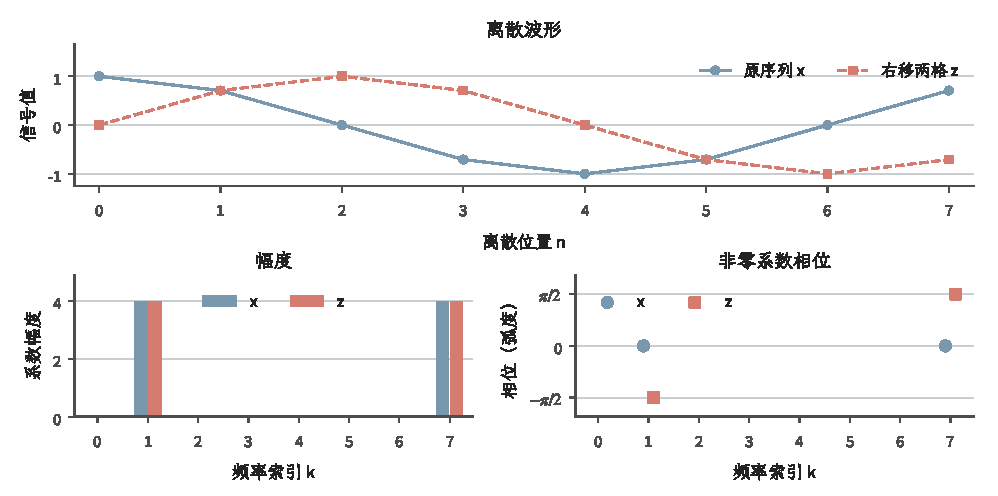
\includegraphics[width=\linewidth]{figures/01-mathematical-preliminaries/03-graphs-and-signals/matplotlib/concepts-dynamics/amplitude-phase.pdf}
  \caption{长度$8$的教学信号$x[n]=\cos(2\pi n/8)$及其循环延迟两格的结果。
  上方波形的峰值位置不同，下方在$k=1,7$的幅度均为$4$，相位却改变。
  相位图只画非零系数；波形连线只帮助观察顺序，不表示已选择连续时间插值。}
  \label{fig:signal-amplitude-phase}
\end{figure*}

这里的复指数坐标来自规则循环平移：每次移动都有统一的方向和步长，DFT同时分解
这些平移。如果位置只通过不规则的连接关联，就不能再根据编号判断谁是“下一格”。
第~\ref{sec:signal-analysis-graph-state-kernels}节将用图上的连接定义变化，
并通过环图说明本节的复指数怎样成为图谱的一个特例。

\subsubsection{周期连续信号的傅里叶表示}

连续时间的一个周期含无穷多个位置，有限个坐标一般不足以完整描述。
周期条件仍把频率限制在整数谐波上，但展开变为无穷级数。
\begin{definition}[周期信号的傅里叶系数与级数]
  \label{def:signal-analysis-fourier-series}
  设$T>0$，$f\in L^2[0,T]$并按周期$T$延拓。在内积
  \[
    \langle f,g\rangle_T=\frac1T\int_0^T f(t)\overline{g(t)}\,\mathrm dt
  \]
  下，复指数$e^{\mathrm i2\pi kt/T}$组成正交归一基。
  \term{傅里叶系数}（Fourier coefficient）为
  \[
    c_k=\frac1T\int_0^T f(t)e^{-\mathrm i2\pi kt/T}\,\mathrm dt,
    \qquad k\in\mathbb Z,
  \]
  相应傅里叶级数写作
  \begin{equation}
    f(t)\sim\sum_{k\in\mathbb Z}c_ke^{\mathrm i2\pi kt/T}.
    \label{eq:signal-analysis-fourier-series}
  \end{equation}
\end{definition}
正交性由对$e^{\mathrm i2\pi(k-j)t/T}$积分得到：$k=j$时归一化积分为$1$，
否则两个端点的指数相同，积分为$0$。完备性给出对称部分和
$S_Kf=\sum_{|k|\leq K}c_ke^{\mathrm i2\pi kt/T}$的$L^2$收敛，
即$T^{-1}\int_0^T|S_Kf-f|^2\to0$。它描述一个周期的平均平方误差，
不能单凭这一结论就在每个$t$写逐点等号。

由正交展开及其极限得到
\begin{equation}
  \frac1T\int_0^T|f(t)|^2\,\mathrm dt
  =\sum_{k\in\mathbb Z}|c_k|^2.
  \label{eq:signal-analysis-continuous-parseval}
\end{equation}
左侧是周期平均功率；单周期能量还要乘以$T$，整轴能量通常无穷。
相应截断误差为$\sum_{|k|>K}|c_k|^2$。
实信号满足$c_{-k}=\overline{c_k}$，延迟$\tau$则把$c_k$变为
$e^{-\mathrm i2\pi k\tau/T}c_k$，幅相的作用与有限情形相同。

逐点重构需增加规则性。例如在一个周期内分段$C^1$、只有有限个跳跃点且单侧极限
存在时，傅里叶级数在连续点趋于$f(t)$，在跳跃点趋于左右极限平均。
这是带条件的结论；不能把均方收敛与逐点或一致收敛互换，
相关性质保持条件可回查第~\ref{chap:mathematical-analysis}章。

取周期$2\pi$的方波：$0<t<\pi$时为$1$，$-\pi<t<0$时为$-1$。
平均值$c_0=0$；对$k\neq0$直接积分，
\[
  c_k=\frac1{2\pi}\left(
    \int_0^\pi e^{-\mathrm ikt}\,\mathrm dt
    -\int_{-\pi}^0 e^{-\mathrm ikt}\,\mathrm dt\right)
  =\frac{1-(-1)^k}{\pi\mathrm ik}.
\]
因此偶数$k$的系数为零，奇数$k$的系数为$2/(\pi\mathrm ik)$，也可配对写成
\[
  \frac4\pi\left(\sin t+\frac{\sin3t}{3}+\frac{\sin5t}{5}+\cdots\right).
\]
连续点处恢复$\pm1$，跳跃点处趋于$0$，无论给原函数的跳跃点赋什么值，
其$L^2$元素和傅里叶系数都不变。Parseval仍给出
$1=(8/\pi^2)\sum_{j=0}^{\infty}(2j+1)^{-2}$。
平均平方误差趋零并不排除跳跃附近的局部振荡；这也是有限谐波近似尖锐边沿时
需要单独观察局部误差的原因。

\subsubsection{整轴离散信号的傅里叶表示}

一条整轴序列不必周期，频率也不再局限于$N$个格点。
但整数$n$使$e^{-\mathrm i(\omega+2\pi)n}=e^{-\mathrm i\omega n}$，
因此频率变量虽然连续，频率表示仍以$2\pi$为周期。
\begin{definition}[离散时间傅里叶变换]
  \label{def:signal-analysis-dtft}
  对$x\in\ell_1(\mathbb Z)$，\term{离散时间傅里叶变换}
  （discrete-time Fourier transform, DTFT）定义为
  \begin{equation}
    X(e^{\mathrm i\omega})=\sum_{n\in\mathbb Z}x[n]e^{-\mathrm i\omega n},
    \qquad \omega\in\mathbb R.
    \label{eq:signal-analysis-dtft}
  \end{equation}
  绝对可和使级数绝对且一致收敛，因而定义连续的$2\pi$周期函数。
\end{definition}
记号$X(e^{\mathrm i\omega})$强调只沿单位圆取值，不在这里假设存在一般复变量的
解析延拓。对$x\in\ell_2$，相同级数改按$L^2([-\pi,\pi])$收敛解释，
所得对象是等价类，不要求每个$\omega$都能按普通级数求值。
两种情形均有系数恢复与能量关系
\begin{align*}
  x[n]&=\frac1{2\pi}\int_{-\pi}^{\pi}
  X(e^{\mathrm i\omega})e^{\mathrm i\omega n}\,\mathrm d\omega,\\
  \sum_n|x[n]|^2&=\frac1{2\pi}\int_{-\pi}^{\pi}|X(e^{\mathrm i\omega})|^2\,\mathrm d\omega.
\end{align*}
在$\ell_1$情形可把绝对收敛级数移入积分，单位复指数的正交性留下第$n$项；
$\ell_2$情形则来自周期$L^2$空间的正交基与Parseval关系。

贯穿例零延拓后的DTFT为
$X(e^{\mathrm i\omega})=1+2e^{-\mathrm i\omega}+e^{-2\mathrm i\omega}$，
它是连续频率曲线。对$N\geq3$，将记录补零到$N$项后计算DFT，
只是读取这条曲线在$\omega=2\pi k/N$上的值。补更多零增加了频率格密度，
没有增加原记录的信息或延长真实观测。
相反，若原序列无穷长，先截取$N$项再作DFT，频谱已受时间截断影响，
不能把结果直接称为完整DTFT的精确采样。
离散频率$\omega$的单位是弧度每样本；样本间隔为$T_s$时才换算成
连续角频率$\Omega=\omega/T_s$，并保留模$2\pi/T_s$的歧义。

\subsubsection{整轴连续信号的傅里叶表示}

整条时间实轴既没有有限长度，也不预设周期，复指数坐标随连续频率变化。
求和相应变成积分，但积分存在性与能量空间延拓仍是两种不同依据。
\begin{definition}[连续时间傅里叶变换]
  \label{def:signal-analysis-continuous-fourier-transform}
  对$f\in L^1(\mathbb R)$，连续时间傅里叶变换为
  \[
    F(\Omega)=\int_{\mathbb R}f(t)e^{-\mathrm i\Omega t}\,\mathrm dt.
  \]
  若还满足$F\in L^1$，逆变换
  \[
    f(t)=\frac1{2\pi}\int_{\mathbb R}F(\Omega)e^{\mathrm i\Omega t}\,\mathrm d\Omega
  \]
  在几乎处处意义下成立，右侧给出连续代表元；在原$f$的连续点也恢复其点值。
  在$L^1\cap L^2$上使用同一积分公式，Plancherel定理将变换唯一延拓到$L^2$，
  满足
  \[
    \int_{\mathbb R}|f(t)|^2\,\mathrm dt
    =\frac1{2\pi}\int_{\mathbb R}|F(\Omega)|^2\,\mathrm d\Omega.
  \]
\end{definition}
一般$L^2$情形的正逆变换按范数极限理解，不保证普通积分在每个频率或时刻存在。
例如改变单个点值不会改变$L^2$元素，变换不可能判断这个点后来被赋成哪个值。
第~\ref{sec:signal-bandlimited-recovery}节将借助带限条件选定连续代表元，
然后才读取采样点；不能对任意等价类未经说明直接采样。

一个可直接积分的例子是$f=\mathbb I_{[0,1]}$：
\[
  F(\Omega)=
  \begin{cases}
    (1-e^{-\mathrm i\Omega})/(\mathrm i\Omega),&\Omega\neq0,\\
    1,&\Omega=0.
  \end{cases}
\]
它在时间上只持续一个单位区间，频谱却没有有限支撑。有限持续时间并不等于带限。
对满足积分条件的实信号，$F(-\Omega)=\overline{F(\Omega)}$；
延迟$\tau$使频谱乘上$e^{-\mathrm i\Omega\tau}$，仍只改相位不改幅度。
这里$\Omega$以弧度每单位时间计，不能与DFT的无量纲索引$k$直接比较。

表~\ref{tab:reader-fourier-objects}汇总四种对象。它们的共同点是复指数坐标，
差别来自索引与周期条件，而不是四个名称可以互换。
\begin{table*}[htbp]
  \centering
  \begin{tabularx}{\linewidth}{lXXX}
    \toprule
    表示 & 输入对象及边界 & 频率坐标 & 成立口径\\
    \midrule
    DFT & $N$项数组，基采用循环索引 & $N$个频率格 & 有限和，可逆\\
    傅里叶级数 & 一个周期上的函数 & 全部整数谐波 & $L^2$均方展开；逐点另需条件\\
    DTFT & 整数轴序列，不要求周期 & 连续且$2\pi$周期 & $\ell_1$下连续；$\ell_2$下为$L^2$等价类\\
    连续傅里叶变换 & 实轴函数，不要求周期 & 连续实频率 & $L^1$积分或$L^2$延拓\\
    \bottomrule
  \end{tabularx}
  \caption{信号对象决定傅里叶表示的频率轴及收敛意义。离散时间不表示频率必然离散，
  频谱周期也不表示原序列周期；有限DFT与整轴DTFT还相差记录范围及边界约定。}
  \label{tab:reader-fourier-objects}
\end{table*}

\subsection{有限信号的代数表示}
\label{sec:signal-analysis-polynomial-arithmetic}

有限序列还有一种不依赖物理频率的表示：把位置写成多项式的幂次。
完整系数、足够多的点值和足够多的互素余数可以描述同一个有限对象。
先确定这些表示的可逆条件，后文才利用它们计算乘积，避免把少算几次乘法
误解为可以少保留几条独立信息。

\subsubsection{位置系数下的多项式表示}

对$\bm x=(x_0,\ldots,x_{m-1})$定义
\[
  X(z)=\sum_{j=0}^{m-1}x_jz^j.
\]
其中$x_j=x[j]$，形式变量$z$首先只记录位置，并不是给系统施加的输入。
长度固定后，序列与次数小于$m$的多项式一一对应；最高位置可以是零，
所以次数未必恰好为$m-1$。例如贯穿记录与核分别对应
$X(z)=1+2z+z^2$和$H(z)=1-z$。
移动一个位置并保留前导零对应乘以$z$，而是否把高次项回绕到低次项，
仍要由边界另行规定。正变换DFT正是$X$在单位根$\omega_N^k$处的求值；
多项式在这里连接位置系数与另一组坐标，并未改变记录本身。

\subsubsection{互异点值下的插值表示}

已知一个多项式在若干位置的值，何时足以恢复全部系数？
答案同时依赖次数界与选点。次数小于$L$的多项式构成$L$维空间。
选取$L$个两两不同的点$a_0,\ldots,a_{L-1}$，求值映射
\[
  E(P)=(P(a_0),\ldots,P(a_{L-1}))
\]
是线性的。若$E(P)=0$，则$P$有$L$个不同根；次数小于$L$的非零多项式
至多有$L-1$个根，因此$P=0$。同维空间间的单射必为双射，
逆映射就是\term{多项式插值}（polynomial interpolation）。

显式恢复可用Lagrange基
\[
  \ell_j(z)=\prod_{\substack{0\leq k<L\\k\neq j}}
  \frac{z-a_k}{a_j-a_k}.
\]
互异性保证分母非零，且$\ell_j(a_k)=\delta_{j,k}$。
故$P$与下式右侧在$L$个点相同、次数都小于$L$，由刚才的唯一性得到
\begin{equation}
  P(z)=\sum_{j=0}^{L-1}P(a_j)\ell_j(z),\qquad\deg P<L.
  \label{eq:signal-analysis-lagrange-interpolation}
\end{equation}
例如一次多项式在$0,1$的值为$1,3$，便恢复为$1(1-z)+3z=1+2z$。
若允许二次项，则$1+2z+c\,z(z-1)$对任意$c$都给出相同两点值，
说明次数界不可省。重复读取同一点也不增加独立约束；导数观测属于另一种插值问题。

代数可逆不等于数值稳定。点值到系数的矩阵逆可能放大测量或舍入误差，
相近选点以及较高次数尤其需要检查条件数，相关判断回用
第~\ref{chap:matrix-analysis}章。单位根的归一化DFT是条件良好的特殊选点，
一般实点并没有同样保证。

\subsubsection{互素余数下的模分解表示}

点值只保留一个数；有时保留关于低次多项式的余数更方便。
余数记录除掉某个模多项式后还剩下的部分，既比完整系数小，又能与其他余数合起来恢复。
为使这种说法有确定含义，先建立除法与唯一性，以下以$F$表示系数域。
域（field）是一套遵守通常加乘运算律、可以加减乘除且非零元素都能作除数的数系；
本节可以先取熟悉的$\mathbb R$或$\mathbb C$。
$F[z]$表示系数在$F$中的有限多项式全体，采用通常的多项式加法与乘法。
\begin{theorem}[多项式带余除法]
  \label{thm:signal-analysis-polynomial-division}
  设$A,M\in F[z]$且$M\neq0$，存在唯一的$Q,R\in F[z]$满足
  \[
    A=QM+R,\qquad\deg R<\deg M.
  \]
  约定零多项式的次数为$-\infty$。
\end{theorem}
\begin{proof}
  若$\deg A<\deg M$，取$Q=0,R=A$。否则设最高次项分别为
  $a_pz^p$与$m_qz^q$，$p\geq q$。域中$m_q$可逆，减去
  $(a_p/m_q)z^{p-q}M$就消掉最高次项。每步次数严格下降，
  有限步后便得到次数小于$\deg M$的余数。

  若还有$A=Q'M+R'$，则$(Q-Q')M=R'-R$。左侧若非零，次数至少为$\deg M$；
  右侧若非零，次数小于$\deg M$，矛盾。因此两侧都为零，$Q=Q'$、$R=R'$。
\end{proof}

对非零$A,B$反复带余除法，
\[
  A=Q_0B+R_1,\qquad B=Q_1R_1+R_2,\qquad\ldots
\]
非零余数的次数严格下降，过程必有限终止。
由$A=Q_0B+R_1$可见，$A,B$的公因式恰好是$B,R_1$的公因式；
逐步应用，最后一个非零余数首项归一化后就是
\term{最大公因式}（greatest common divisor）。
从最后一个等式向前回代，每个余数均为$A,B$的多项式线性组合，得到
\begin{equation}
  U(z)A(z)+V(z)B(z)=\gcd(A,B).
  \label{eq:signal-analysis-polynomial-bezout}
\end{equation}
这是Bézout恒等式。互素表示最大公因式为非零常数，等价于存在$U,V$使左侧为$1$。
例如在$\mathbb R[z]$中，
\[
  z^2+1=(z+1)(z-1)+2,\qquad
  1=\tfrac12(z^2+1)-\tfrac12(z+1)(z-1).
\]
它既证明$z-1$与$z^2+1$互素，也提供了后面重构所需的逆元。

把余数记为$A\bmod M$，把相差$M$倍数的多项式看成同一个
\term{剩余类}（residue class），记为$[A]_M$。
当$M=z-a$时，除法式在$z=a$处给出
$A(z)=Q(z)(z-a)+A(a)$，所以点值恰好是关于一次模的常数余数。
多个余数如何恢复同一对象，由下述定理回答。
\begin{theorem}[多项式中国剩余定理]
  \label{thm:signal-analysis-polynomial-crt}
  设非恒定多项式$m_1,\ldots,m_s\in F[z]$两两互素，令$M=\prod_{j=1}^s m_j$。
  映射
  \[
    [A]_M\longmapsto([A]_{m_1},\ldots,[A]_{m_s})
  \]
  是环同构（ring isomorphism），即双射并且保持加法和乘法；
  余数类相加或相乘，都是先作多项式运算再对相应的模取余。
  因此全部余数唯一确定次数小于$\deg M$的代表元$A\bmod M$。
\end{theorem}
\begin{proof}
  若$A-B$是$M$的倍数，它也是各$m_j$的倍数，故映射不依赖代表元；
  取余还保持加法与乘法。若$A,B$的各个余数都相同，则每个$m_j$整除$A-B$。
  为证明乘积也整除，先设互素的$a,b$均整除$q$，写$q=ac$。
  由$ua+vb=1$有$c=uac+vbc=uq+vbc$，所以$b$整除$c$，从而$ab$整除$q$。
  两两互素时，若某多项式分别与$a,b$互素，将对应Bézout等式相乘即可证明
  它与$ab$互素。反复使用前述整除结论，便有$M\mid(A-B)$，映射为单射。

  给定任意余数$r_j$，令$M_j=M/m_j$。互素性与Bézout恒等式给出
  $u_jM_j+v_jm_j=1$。因此$e_j=u_jM_j$关于$m_j$的余数是$1$，
  关于其他$m_k$的余数是$0$。取
  \[
    A=\sum_{j=1}^s r_je_j
  \]
  即具有全部指定余数，故映射满射。最后对$M$取余，带余除法给出唯一的
  次数小于$\deg M$代表元。
\end{proof}

互素性使各份信息能够独立拼合，次数界使模意义下的唯一性成为原多项式的唯一性。
例如知道$P\bmod z$和$P\bmod(z-1)$可以恢复一次多项式，却无法区分
$P$与$P+c\,z(z-1)$；反复使用同一个模更不增加信息。
在模$z^N-1$下，$z^{N+s}$与$z^s$属于同一剩余类，因而高次系数按模$N$合并。
这个规则将编码循环边界，但此时还没有计算两个信号的乘积。
余数恢复如何减少卷积计算，留到第~\ref{sec:signal-analysis-fast-transforms}节。

\section{信号的运算与映射}
\label{sec:signal-operations-maps}

表示回答同一条信号怎样描述，运算则回答它怎样变成另一条信号。
移动、反转、缩放及叠加是基本操作；输入输出映射把这些操作组合为滤波或历史响应，
相关则比较模板与局部片段。线性、平移不变和不使用未来输入分别约束不同性质，
不能因某个操作具有其中之一就替它补上另外两项。快速算法也必须在目标映射明确后讨论。

\subsection{信号的基本运算}

为避免对称波形掩盖方向差异，本节固定一个非对称三角脉冲：
\begin{equation}
  x(t)=
  \begin{cases}
    2t,&0\leq t\leq1,\\
    3-t,&1<t\leq3,\\
    0,&\text{其余位置}.
  \end{cases}
  \label{eq:signal-asymmetric-wave}
\end{equation}
它在$t=1$达到峰值$2$，上升历时$1$、下降历时$2$，
能量为$\int_0^1 4t^2\,\mathrm dt+\int_1^3(3-t)^2\,\mathrm dt=4$。
图~\ref{fig:signal-basic-operations}始终用它作参照。

\subsubsection{平移下的位置变化}

连续时间的延迟$\tau$写成$(T_\tau x)(t)=x(t-\tau)$；
离散时间沿用$(T_rx)[k]=x[k-r]$，只允许整数$r$。
正参数使已有特征推迟出现，负参数使其提前。
例如$x(t-1)$的峰值从$t=1$移到$t=2$，支撑从$[0,3]$移到$[1,4]$。
长度$N$的循环延迟则为$x[(k-r)\bmod N]$，越过右端的值回到左端。
对有限非循环记录，必须先按第~\ref{sec:signal-objects-structure}节约定延拓，
再决定是否裁剪到原窗口，不能将丢出窗口的值自动送回首端。

对整轴上同一信号空间的$x,z$，换元给出
$\langle T_\tau x,T_\tau z\rangle=\langle x,z\rangle$；
离散情形用求和换标，循环情形用有限位置的置换得到相同结论。
相应的整轴$L^p$、$\ell_p$范数和能量均不变。
但固定窗口$[0,3]$内，$x(t-1)$只保留原波形的$[0,2]$部分，
窗口能量从$4$降为$11/3$。这是裁剪改变了观测范围，不是平移在整轴上消耗了能量。

\subsubsection{反转下的方向变化}

时间反转定义为$(Rx)(t)=x(-t)$，离散整轴上为$(Rx)[k]=x[-k]$。
它把发生次序沿原点翻转，式~\eqref{eq:signal-asymmetric-wave}的支撑变为$[-3,0]$，
峰值位于$-1$。有限数组通常说的“反序”却是
$x_{\mathrm{rev}}[k]=x[N-1-k]$，$0\leq k<N$；
按整轴零延拓，它等于$T_{N-1}Rx$，是在反转后平移回记录窗口。
循环反转则用$x[(-k)\bmod N]$，位置$0$保持不动，与数组反序也不同。

反转不改变幅值符号；取负$-x(t)$才把正值变成负值，复共轭
$\overline{x(t)}$只改变每个位置的虚部符号。
例如非对称非负波形反转后仍非负，取负后却非正；
复信号$(1+\mathrm i)\mathbb I_{[0,1]}(t)$的共轭仍支持在$[0,1]$，
而时间反转支持在$[-1,0]$，两者不能互换。
换元$t\mapsto-t$或$k\mapsto-k$表明整轴反转保持内积、范数与能量。
后文卷积中的核反转、相关改写中额外的复共轭，将分别使用这里的两项操作。

\subsubsection{幅值缩放与信号叠加}

标量倍乘$(ax)(t)=a\,x(t)$改变幅值，逐点相加
$(x+z)(t)=x(t)+z(t)$组合同时位置的值。对任意范数，
$\|ax\|=|a|\|x\|$，故能量为$E_{ax}=|a|^2E_x$；
若长期平均功率存在，也乘以$|a|^2$。
图中的$2x(t)$保持峰值时刻和支撑不变，峰值变为$4$，能量变为$16$，
与把时间压缩一半不是一件事。

叠加时的能量含有干涉项。沿用第一变量线性的内积，
\[
  \|ax+bz\|_2^2
  =|a|^2\|x\|_2^2+|b|^2\|z\|_2^2
   +2\operatorname{Re}\!\left(a\overline b\,\langle x,z\rangle\right).
\]
正交信号的能量直接相加；一般信号可能相互增强或抵消。
有限记录$x=(1,2,1)$与$z=(1,0,-1)$正交，故$\|x+z\|_2^2=6+2=8$；
取$z=x$则$\|x+z\|_2^2=24$而不是$12$，取$z=-x$更会完全抵消。

多通道统一缩放是$a\bm x[k]$，逐通道缩放是对角矩阵$\bm D\bm x[k]$，
一般矩阵$\bm B\bm x[k]$还混合不同通道。
后两种操作不必按同一比例改变总能量；
只有$\bm B^*\bm B=\bm I$时才对所有输入保持欧氏通道能量。
这同时说明“组合两路传感器”必须给出矩阵及通道单位，不能默认为没有损失的重命名。

\subsubsection{时间缩放与尺度变化}

对连续时间和$a\neq0$，定义$y(t)=x(at)$。
$|a|>1$把时间压缩，$0<|a|<1$把时间伸展，$a<0$还附带时间反转。
若$x$的某个特征位于$t_0$，$y$中的同一特征就位于$t_0/a$。
图中的$x(2t)$峰值仍为$2$，但峰值时刻变为$1/2$，支撑缩短为$[0,3/2]$。
对有限能量信号，换元$s=at$给出
\[
  E_y=\int_{\mathbb R}|x(at)|^2\,\mathrm dt
  =\frac1{|a|}\int_{\mathbb R}|x(s)|^2\,\mathrm ds=\frac{E_x}{|a|}.
\]
因此$x(2t)$的能量为$2$；幅值未变，累计时间却减少。
若需要缩放时间同时保持二范数，应使用$|a|^{1/2}x(at)$。
当平均功率存在时，同样换元并把平均窗口一起缩放，得到$P_y=P_x$，
这与总能量的尺度因子并不矛盾。

整数索引不能随意替换成实数。$x[Mk]$对正整数$M$有定义，表示每$M$项抽取一项；
$x[k/M]$在$k$不是$M$倍数时没有已有样本可读。
插零上采样先规定$u[k]=x[k/M]$在$M\mid k$时成立、其余位置为零，
再由插值规则生成中间值。插零本身不是已经恢复连续波形，抽取也没有
连续时间换元那样的通用能量比例。采样后保留什么信息，须在
第~\ref{sec:signal-analysis-sampling}节另行判断。
\begin{figure*}[htbp]
  \centering
  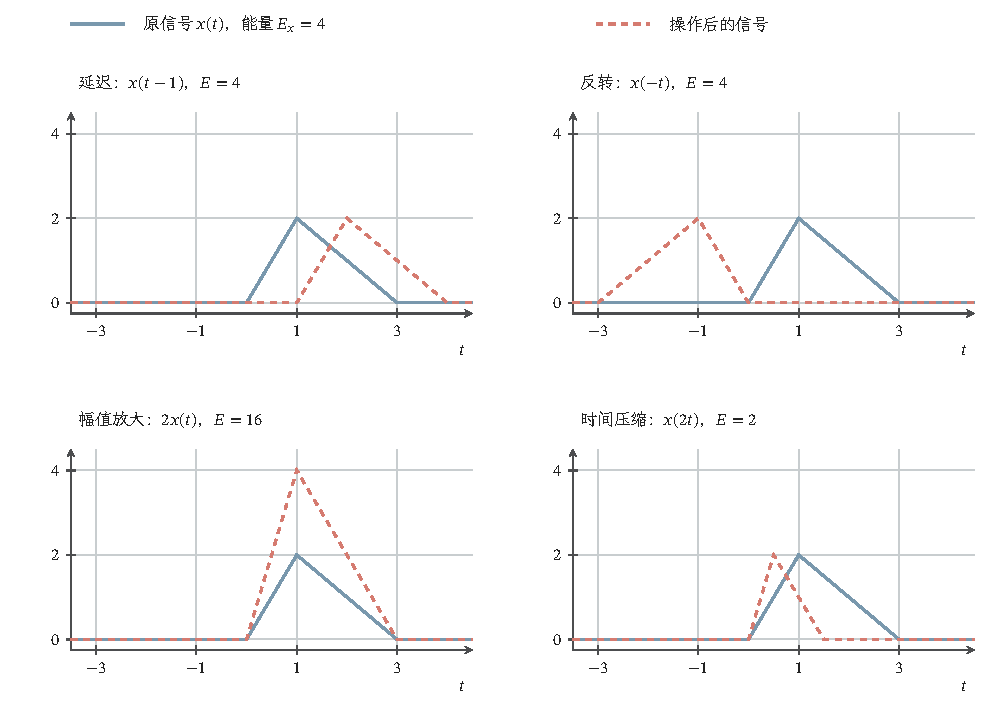
\includegraphics[width=\linewidth]{figures/01-mathematical-preliminaries/03-graphs-and-signals/tikz/signals/basic-operations.pdf}
  \caption{对同一非对称三角脉冲分别延迟、反转、放大幅值和压缩时间。
  每幅图的蓝线均为式~\eqref{eq:signal-asymmetric-wave}的原信号，红线为指定操作结果，
  横轴为时间、纵轴为幅值，坐标尺度一致。平移和反转保持整轴能量$4$，幅值乘$2$使能量变为$16$，
  时间压缩为一半使能量变为$2$；各图均在整轴零值背景下观察，不作窗口裁剪。}
  \label{fig:signal-basic-operations}
\end{figure*}

\subsection{信号的输入输出映射}
\label{sec:signal-input-output-maps}
\label{sec:signal-analysis-discrete-filtering}

一个系统是把输入信号映为输出信号的规则$y=\mathcal Hx$。
在有限位置上，线性规则可写成$y[n]=\sum_r K[n,r]x[r]$，
其中$K[n,r]$说明位置$r$的单位输入怎样影响位置$n$的输出。
整轴表达还需收敛条件，不能仅凭这个形式就交换无穷求和。
若输入、输出有$d_{\mathrm{in}}$和$d_{\mathrm{out}}$个通道，
则$K[n,r]$应为$d_{\mathrm{out}}\times d_{\mathrm{in}}$矩阵，
矩阵乘法负责混合通道，求和负责汇总时间位置，两者职责不同。

这里的因果性只表示“不读取未来输入”：若两条输入在所有$r\leq n$的位置相同，
则它们在时刻$n$的输出必须相同。对可用脉冲逐项检验的线性核映射，
这等价于$K[n,r]=0$在$r>n$时成立。
它不是第~\ref{chap:causal-inference}章用干预定义的因果响应；
只按过去顺序计算一个预测量，不会自动证明其统计关系具有干预含义。

\subsubsection{线性时不变条件下的卷积映射}
\label{sec:signal-analysis-lti-convolution}

如果改变输入幅值可以按比例叠加，而且同一个局部输入移到哪里都触发同形响应，
就有希望只保存一条响应核。两项要求需要分别定义。
\begin{definition}[线性时不变系统]
  \label{def:signal-analysis-lti-system}
  设输入、输出信号类为平移封闭的向量空间。若对任意标量$a,b$及输入$x,z$有
  $\mathcal H(ax+bz)=a\mathcal Hx+b\mathcal Hz$，称$\mathcal H$线性。
  若对每个整数$r$有
  \[
    \mathcal H(T_rx)=T_r(\mathcal Hx),
  \]
  称其具有\term{平移不变性}（shift invariance）。
  同时满足两者的系统称为线性时不变系统（linear time-invariant system, LTI）。
\end{definition}
这里输入整体移动后输出同样移动，并不是输出保持在原位置。
逐点平方$\mathcal Hx[n]=x[n]^2$平移不变却不线性，
位置加权$\mathcal Hx[n]=n\,x[n]$线性却不平移不变。
是否在每个位置调用了同一段程序，不足以替代这两项等式。

令$h=\mathcal H\delta$，称为\term{脉冲响应}（impulse response）。
有限支撑输入可按式~\eqref{eq:signal-analysis-impulse-expansion}作有限展开，
线性性与平移不变性给出
\begin{align}
  (\mathcal Hx)[n]
  &=\mathcal H\left(\sum_r x[r]T_r\delta\right)[n]\notag\\
  &=\sum_r x[r](T_rh)[n]=\sum_r x[r]h[n-r].
  \label{eq:signal-analysis-lti-convolution}
\end{align}
它把各位置输入所触发的响应相加。
对$x\in\ell_1(\mathbb Z)$，还需
$\mathcal H:\ell_1\to\ell_1$为有界线性且平移不变的算子，
即存在常数$C$使$\|\mathcal Hx\|_1\leq C\|x\|_1$。
令$x^{(K)}=\sum_{|r|\leq K}x[r]T_r\delta$，则$x^{(K)}\to x$于$\ell_1$，
有界性使$\mathcal Hx^{(K)}\to\mathcal Hx$。同时$h=\mathcal H\delta\in\ell_1$，
且
\[
  \sum_n\sum_r|x[r]h[n-r]|=\|x\|_1\|h\|_1<\infty.
\]
因此卷积和绝对收敛，有限截断的卷积也在$\ell_1$中趋于该和，
从而式~\eqref{eq:signal-analysis-lti-convolution}延伸到全部$\ell_1$输入。
不能省略连续性，直接把仅对有限和成立的代数线性搬进无穷和。

这种求和称为\term{离散卷积}（discrete convolution），规则网格上也可用同一结构。
\begin{definition}[网格上的离散卷积]
  \label{def:signal-analysis-discrete-convolution}
  对$x,h\in\ell_1(\mathbb Z^d)$，定义
  \begin{equation}
    (x*h)[\bm n]=\sum_{\bm r\in\mathbb Z^d}x[\bm r]h[\bm n-\bm r].
    \label{eq:signal-analysis-discrete-multidimensional-convolution}
  \end{equation}
  这里$\bm n,\bm r$为网格位置，$h$称为\term{卷积核}（convolution kernel）。
  各位置的和绝对收敛，输出仍属于$\ell_1(\mathbb Z^d)$。
\end{definition}
存在性可直接检查：对非负项换序并令$\bm s=\bm n-\bm r$，有
\[
  \sum_{\bm n}\sum_{\bm r}|x[\bm r]h[\bm n-\bm r]|
  =\left(\sum_{\bm r}|x[\bm r]|\right)
   \left(\sum_{\bm s}|h[\bm s]|\right)<\infty.
\]
所以每个内层和均有限，并得到
$\|x*h\|_1\leq\|x\|_1\|h\|_1$。
核为有限支撑时，对任何逐点有限的输入也可作有限和，但输出不因此必属$\ell_1$。
一维记法为
\begin{equation}
  (x*h)[n]=\sum_{r\in\mathbb Z}x[r]h[n-r].
  \label{eq:signal-analysis-linear-convolution}
\end{equation}
固定$n$后，$r$增加时核索引$n-r$减小，这就是核的反向读取。
令$s=n-r$可得$(x*h)[n]=\sum_s h[s]x[n-s]=(h*x)[n]$，故有交换律；
绝对可和等允许换序的条件还给出结合律和分配律。
若$h[r]=0$对所有$r<0$成立，则$y[n]=\sum_r h[r]x[n-r]$只用当前及过去输入，
系统因果；一般LTI则不必因果，例如三点中心均值会使用$x[n+1]$。

连续输入的局部贡献改用积分累计。
\begin{definition}[连续卷积]
  \label{def:signal-analysis-continuous-convolution}
  设$f,g\in L^1(\mathbb R^d)$，定义
  \begin{equation}
    (f*g)(\bm t)=\int_{\mathbb R^d}f(\bm\tau)g(\bm t-\bm\tau)\,\mathrm d\bm\tau.
    \label{eq:signal-analysis-continuous-convolution}
  \end{equation}
  积分对几乎处处的$\bm t$绝对收敛，并定义$L^1(\mathbb R^d)$中的元素。
\end{definition}
由定理~\ref{thm:analysis-tonelli-fubini}，对非负函数换序并平移换元，
\[
  \int_{\mathbb R^d}\int_{\mathbb R^d}
  |f(\bm\tau)g(\bm t-\bm\tau)|\,\mathrm d\bm\tau\,\mathrm d\bm t
  =\|f\|_{L^1}\|g\|_{L^1}<\infty.
\]
内层积分因而几乎处处有限，且$\|f*g\|_{L^1}\leq\|f\|_{L^1}\|g\|_{L^1}$。
换元和换序同样给出交换律、结合律，但$L^1$假设不保证每个指定点的积分都有限。
这里定义的是两个普通可积函数的卷积，并非所有连续LTI算子都具有普通$L^1$核。
例如恒等映射是LTI，它的单位脉冲响应可用Dirac分布（Dirac distribution）
$\delta_0$描述。这里“分布”采用广义函数的用语：这个对象作用于光滑紧支撑的
测试函数$\phi$时返回$\delta_0(\phi)=\phi(0)$，也就是零点单位质量对$\phi$的积分。
对这样的$f$，卷积让它读取$\tau\mapsto f(t-\tau)$在零点的值，
于是$(f*\delta_0)(t)=f(t)$，正好实现恒等映射。
普通函数$\mathbb I_{\{0\}}$的Lebesgue积分却为零，不能承担这种单位质量，
所以不能把离散$\delta[k]$直接当作连续可积核。
当前不调用一般分布理论来证明所有连续系统的核表示。

\begin{example}[区间重叠产生三角形响应]
  \label{ex:signal-analysis-continuous-overlap}
  取$f(t)=g(t)=\mathbb I_{[0,1]}(t)$。两因子同时为$1$要求
  $\tau\in[0,1]\cap[t-1,t]$，因此
  \[
    (f*g)(t)=
    \begin{cases}
      t,&0\leq t\leq1,\\
      2-t,&1<t\leq2,\\
      0,&\text{其余位置}.
    \end{cases}
  \]
  输出先随重叠长度增大而上升，再随重叠减小而下降。
  二维指示函数的相应积分计算重叠面积，一般带符号核则计算加权贡献，
  不能都解释为几何大小。
\end{example}
图~\ref{fig:reader-continuous-convolution-overlap}区分输出位置$t$和积分变量$\tau$。
三角形输出不是把两个输入图形相加，而是把每个$t$处的重叠长度汇成曲线。
\begin{figure*}[htbp]
  \centering
  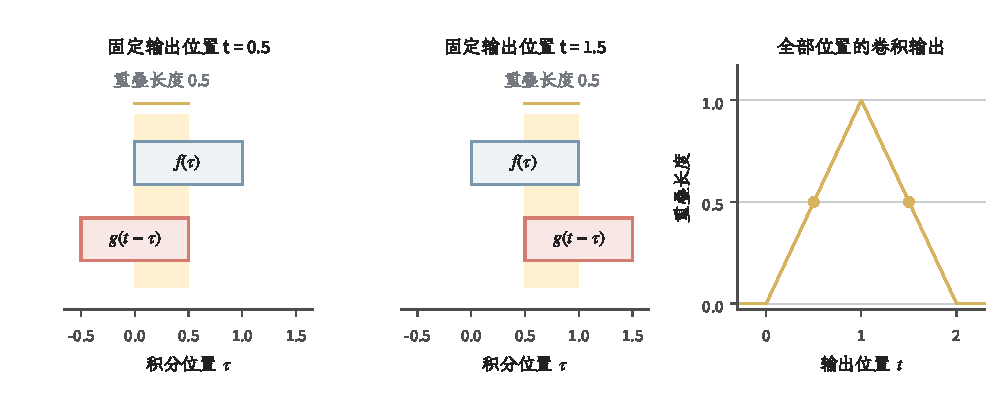
\includegraphics[width=\linewidth]{figures/01-mathematical-preliminaries/03-graphs-and-signals/matplotlib/teaching-dynamics/continuous-convolution-overlap.pdf}
  \caption{教学函数$f=g=\mathbb I_{[0,1]}$的连续卷积。左两图分别固定$t=0.5$与$t=1.5$，
  蓝色为$f(\tau)$的支撑，红色为$g(t-\tau)$的支撑，黄色重叠长度均为$0.5$。
  右图汇总全部$t$处的重叠长度，在$t=1$时达到$1$。
  左图横轴$\tau$用于积分，右图横轴$t$标记输出位置。}
  \label{fig:reader-continuous-convolution-overlap}
\end{figure*}

回到有限输入。若$x,h$的支撑分别为$0,\ldots,m-1$和$0,\ldots,r-1$，
零延拓线性卷积只可能在$0,\ldots,m+r-2$非零，完整输出长度为$m+r-1$。
贯穿例逐项为
\begin{align*}
  (x*h)[0]&=1,\\
  (x*h)[1]&=2-1=1,\\
  (x*h)[2]&=1-2=-1,\\
  (x*h)[3]&=-1.
\end{align*}
即
\begin{equation}
  \bm x*\bm h=(1,1,-1,-1).
  \label{eq:signal-analysis-running-linear-convolution}
\end{equation}
这个核计算当前值减去前一个值，首尾还包含零延拓带来的跳变。
长度$N$的循环索引则在一个周期内求和：
\begin{equation}
  (x*_Nh)[n]=\sum_{r=0}^{N-1}x[r]h[(n-r)\bmod N],
  \qquad n=0,\ldots,N-1.
  \label{eq:signal-analysis-circular-convolution}
\end{equation}
\begin{definition}[循环卷积]
  \label{def:signal-analysis-circular-convolution}
  对长度$N$的实或复序列，式~\eqref{eq:signal-analysis-circular-convolution}
  定义其\term{循环卷积}（circular convolution），输出仍有$N$项。
  它在有限循环索引集上求和，不是两条周期延拓序列在整数轴上的无穷卷积。
\end{definition}
把$h$补成$(1,-1,0)$并取$N=3$，得到$x*_3h=(0,1,-1)$。
完整线性卷积的末项$-1$回绕到首项，与$1$相消；不是直接删掉了末项。
若对两条周期序列在整轴无穷求和，同一贡献会被重复无穷次。
图~\ref{fig:signal-convolution-boundaries}对比零延拓与循环边界下的输出。
\begin{figure}[!htb]
  \centering
  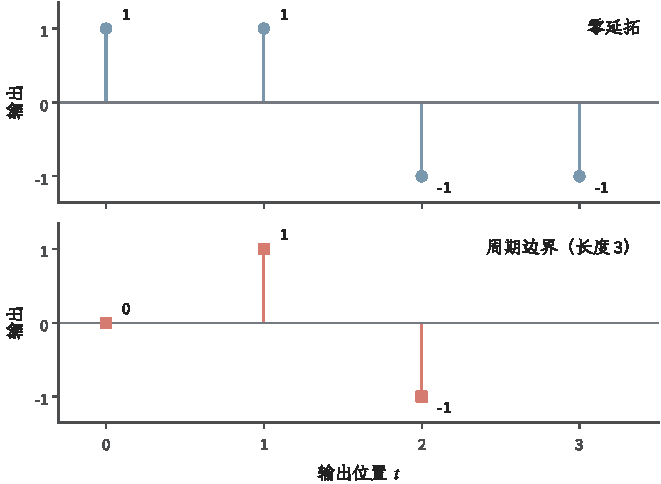
\includegraphics[width=\linewidth]{figures/01-mathematical-preliminaries/03-graphs-and-signals/matplotlib/dynamics/convolution-boundaries.pdf}
  \caption{输入$(1,2,1)$与核$(1,-1)$的边界比较。蓝色圆点采用零延拓，给出四项线性卷积；
  红色方点采用长度$3$的循环边界，末项$-1$回到首项并与$1$抵消。
  连线只指示离散数值的顺序，不定义整数之间的信号值。}
  \label{fig:signal-convolution-boundaries}
\end{figure}

固定输入输出位置后，线性卷积是Toeplitz矩阵乘法，循环卷积是循环矩阵乘法。
例如同一个贯穿例给出
\begin{gather*}
  \begin{bmatrix}
    1&0&0\\-1&1&0\\0&-1&1\\0&0&-1
  \end{bmatrix}
  \begin{bmatrix}1\\2\\1\end{bmatrix}
  =\begin{bmatrix}1\\1\\-1\\-1\end{bmatrix},\\
  \begin{bmatrix}1&0&-1\\-1&1&0\\0&-1&1\end{bmatrix}
  \begin{bmatrix}1\\2\\1\end{bmatrix}
  =\begin{bmatrix}0\\1\\-1\end{bmatrix}.
\end{gather*}
重复对角线反映参数共享，边界则改变矩阵首尾行。
无限网格或循环群上的平移不变性是精确的；有限区间采用零填充、反射或截取后，
通常不再具有同一意义的全局平移不变性。

“valid”只选择核完全落在已知输入内的输出。
按$h[0],\ldots,h[r-1]$的因果索引，当$m\geq r$时保留$n=r-1,\ldots,m-1$，
共$m-r+1$项；$m<r$时没有这样的输出。
保持输入长度的“same”还需指定左右填充及截取位置，不能只凭名称确定。
表~\ref{tab:signal-boundary-conventions}将延拓和输出选择分开，
后文FFT也必须遵守同一约定。
\begin{table*}[!htb]
  \centering
  \begin{tabularx}{\linewidth}{lXXX}
    \toprule
    约定 & 区间外输入 & 保留输出 & 贯穿例\\
    \midrule
    完整线性卷积 & 零延拓 & $0,\ldots,m+r-2$ & $(1,1,-1,-1)$\\
    有效区间选段 & 不使用区间外值 & $r-1,\ldots,m-1$，$m\geq r$ & $(1,-1)$\\
    $N$点循环卷积 & 周期边界 & $0,\ldots,N-1$ & $N=3$时$(0,1,-1)$\\
    \bottomrule
  \end{tabularx}
  \caption{边界延拓与输出选段。$m$为输入长度，$r$为核长度，使用本章因果核索引。
  有效选段不是另一种卷积定义，循环边界也不是零边界的近似。}
  \label{tab:signal-boundary-conventions}
\end{table*}

有了有限DFT，循环卷积可在频率坐标中逐项计算。
\begin{theorem}[离散循环卷积定理]
  \label{thm:signal-analysis-circular-convolution-theorem}
  设$x,h$为长度$N$的复序列，采用式~\eqref{eq:signal-analysis-dft}的约定，则
  \[
    \widehat{x*_Nh}[k]=\widehat x[k]\widehat h[k],\qquad k=0,\ldots,N-1.
  \]
\end{theorem}
\begin{proof}
  令$a=(n-r)\bmod N$，直接换有限求和的索引，
  \begin{align*}
    \widehat{x*_Nh}[k]
    &=\sum_{n=0}^{N-1}\sum_{r=0}^{N-1}
      x[r]h[(n-r)\bmod N]\omega_N^{kn}\\
    &=\sum_{r=0}^{N-1}\sum_{a=0}^{N-1}
      x[r]h[a]\omega_N^{k(r+a)}\\
    &=\left(\sum_{r=0}^{N-1}x[r]\omega_N^{kr}\right)
      \left(\sum_{a=0}^{N-1}h[a]\omega_N^{ka}\right).
  \end{align*}
  固定$r$后，$n$遍历一个周期使$a$也恰遍历一个周期。
  即使$n$与$r+a$相差$N$的整数倍，$\omega_N^{kN}=1$仍使指数相同。
  最后两项分别为$\widehat x[k]$与$\widehat h[k]$。
\end{proof}
于是
\begin{equation}
  x*_Nh=\mathcal F_N^{-1}\bigl(\mathcal F_N(x)\odot\mathcal F_N(h)\bigr).
  \label{eq:signal-analysis-frequency-domain-convolution}
\end{equation}
若$\bm C_h$为循环卷积矩阵，定理对所有$x$成立，故
$\bm F\bm C_h=\operatorname{diag}(\widehat{\bm h})\bm F$，从而
$\bm C_h=\bm F^{-1}\operatorname{diag}(\widehat{\bm h})\bm F$。
这完整说明DFT如何对角化循环卷积：核的DFT系数是各频率模式的特征值。
要用它得到完整线性卷积，两个输入均须补零到
\begin{equation}
  N\geq m+r-1.
  \label{eq:signal-analysis-linear-padding-condition}
\end{equation}
因为所有非零输出索引此时都小于$N$，不会回绕。
$N\geq\max(m,r)$只保证装下输入，不保证装下输出。

整轴频率响应改用DTFT。若$h\in\ell_1$或具有有限支撑，
即使复指数$x[n]=e^{\mathrm i\omega n}$自身不在$\ell_1$中，仍有绝对收敛的和
\[
  (x*h)[n]=\sum_r h[r]e^{\mathrm i\omega(n-r)}
  =e^{\mathrm i\omega n}\sum_r h[r]e^{-\mathrm i\omega r}.
\]
输出保持频率，只乘以
\begin{equation}
  H(e^{\mathrm i\omega})=\sum_r h[r]e^{-\mathrm i\omega r},
  \label{eq:signal-analysis-filter-frequency-response}
\end{equation}
即\term{频率响应}（frequency response）。模长给出放大或衰减，相角给出该模式的
相位变化；除非相位随频率具有相应线性形式，不能将所有频率的相位变化都叫同一时间延迟。
对$x,h\in\ell_1$，绝对可和允许换序，直接得到
$Y(e^{\mathrm i\omega})=X(e^{\mathrm i\omega})H(e^{\mathrm i\omega})$。
同理，连续$L^1$卷积的傅里叶变换为$F(\Omega)G(\Omega)$，
其积分换序由前面的绝对积分界保证。

贯穿核的响应为$H(e^{\mathrm i\omega})=1-e^{-\mathrm i\omega}$，
模长为$2|\sin(\omega/2)|$。常量模式$\omega=0$被消去，低频缓变被削弱，
较高频的差异更突出；这解释了它为何是一阶差分，而有限输入首尾仍受延拓影响。

多通道卷积将标量核换成矩阵核：
\begin{equation}
  y_a[n]=\sum_{b=1}^{d_{\mathrm{in}}}\sum_{r\in\mathbb Z}
  H_{a,b}[r]x_b[n-r],
  \qquad a=1,\ldots,d_{\mathrm{out}}.
  \label{eq:signal-multichannel-convolution}
\end{equation}
各$H_{a,b}\in\ell_1$、各$x_b\in\ell_1$时，有限通道求和与前述界保证存在性；
有限核则在每个位置作有限计算。相同输入输出通道数且$\bm H[r]$总是对角矩阵时，
各通道独立滤波；非对角元素允许输入通道$b$影响输出通道$a$。
频域关系相应为$\widehat{\bm y}[k]=\widehat{\bm H}[k]\widehat{\bm x}[k]$，
每个频率上是矩阵乘向量，不是把所有通道分别做一个标量乘法。

无时间记忆的特例$\bm H[0]=\bm B$、其余为零，只在同一时刻混合通道。
取式~\eqref{eq:signal-multichannel-record}中的记录及
$\bm B=\begin{bmatrix}1&1\\1&-1\end{bmatrix}$，有
\[
  \bm Y=\bm X\bm B^\top
  =\begin{bmatrix}1&1\\3&1\\3&-1\end{bmatrix}.
\]
如图~\ref{fig:signal-channel-mixing}所示，输出第一通道为和，第二通道为差，
三个时间位置未变。总能量从$11$变为$22$，因为$\bm B^\top\bm B=2\bm I$；
用$\bm B/\sqrt2$才保持能量。混合前若两路未按时间对齐，矩阵计算本身不会修正偏移。
\begin{figure*}[htbp]
  \centering
  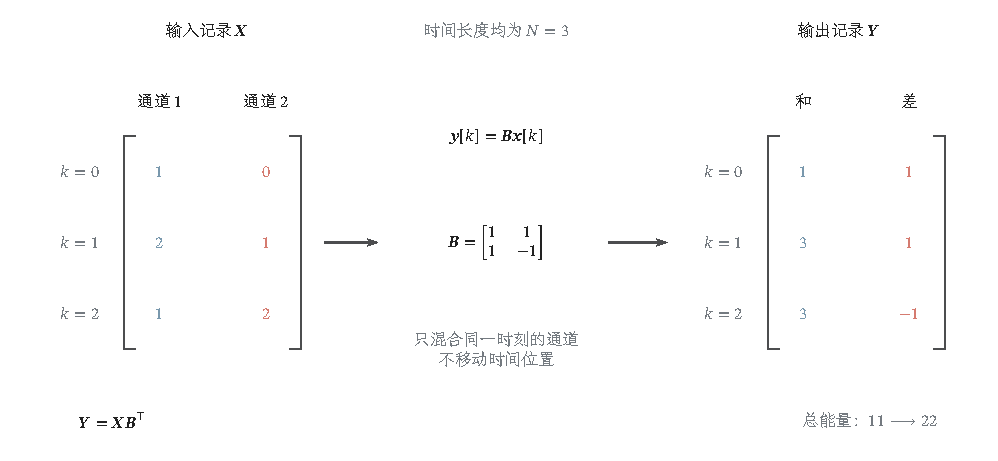
\includegraphics[width=\linewidth]{figures/01-mathematical-preliminaries/03-graphs-and-signals/tikz/signals/channel-mixing.pdf}
  \caption{同一双通道三时刻记录的轴与混合。左侧行标记时间、列标记通道；
  中间矩阵$\bm B$对每一行对应的同时读数取和与差，右侧时间轴长度仍为$3$。
  通道混合不是时间平移，也不意味着两个输入通道独立；这里只使用当前时刻的值。}
  \label{fig:signal-channel-mixing}
\end{figure*}

\subsubsection{线性时变条件下的历史映射}

设备增益随时刻变化时，同样的脉冲在不同时间可能触发不同响应，线性却仍可成立。
用已给定的两时刻核表示
\begin{equation}
  \bm y[n]=\sum_{r\leq n}\bm K[n,r]\bm x[r].
  \label{eq:signal-given-time-varying-kernel}
\end{equation}
有限历史窗口中它是有限和；无限历史中则需另行保证收敛，
例如对有界输入可要求$\sum_{r\leq n}\|\bm K[n,r]\|<\infty$。
求和只取$r\leq n$规定因果性，矩阵维度仍为
$d_{\mathrm{out}}\times d_{\mathrm{in}}$。
核事先固定、不随输入改变时，该表达满足叠加。
若同时满足$\bm K[n+s,r+s]=\bm K[n,r]$，才只依赖滞后$n-r$，
并可记成固定卷积核；只因它累加历史，不能省掉这项条件。

例如令$a[n]$在偶数时为$1$、奇数时为$2$，
$y[n]=a[n](x[n]+\tfrac12x[n-1])$。
它的两时刻核仅在$r=n,n-1$非零，且取值随绝对时刻$n$变化。
输入$\delta[n]$在时刻$0$给出$1$，将输入延迟一格后，时刻$1$的输出却为$2$，
而原输出延迟一格在该处仍为$1$，因此不平移不变。
相反，事先给定$h[0]=0$、$h[r]=2^{-(r-1)}$（$r\geq1$）及负索引为零，
就定义了一个有衰减记忆的固定卷积核。对零延拓$x=(1,2,1)$，
从时刻$0$起的前四项输出为$(0,1,5/2,9/4)$，每次使用相同的滞后权重。

这些例子只需知道输入输出核，不需先引入内部状态。
第~\ref{sec:signal-analysis-state-history-kernels}节将从状态演化构造固定核与两时刻核，
并区分初始状态的自由响应、直接项和输入驱动项。
那里的有序矩阵乘积解释核从何而来；本节检验的是给定核定义了什么映射。
若另加一个与输入无关且非零的自由响应，总映射一般是仿射而非线性，
不能仅因输入驱动部分线性就忽略这一差别。

\subsubsection{非线性条件下的输入依赖映射}

核如果根据当前输入调整，冻结核后的一次矩阵乘法也不能代表整个映射。
最简单的例子是$(\mathcal Hx)[n]=x[n]^2$：对$x[n]=1$，
$\mathcal H(2x)[n]=4\neq2\mathcal Hx[n]$，故不线性。
但$\mathcal H(T_rx)[n]=x[n-r]^2=T_r(\mathcal Hx)[n]$，所以它仍平移不变，
且只使用当前值，满足这里的因果性。

再看输入依赖门控
\[
  y[n]=g(x[n])x[n],\qquad g(v)=\frac1{1+e^{-v}}
\]
（此例取实数输入）。门控是由当前输入决定的权重。
输入$1$与$2$得到的比例分别是$g(1)$与$g(2)$，两者不同，
所以$y(2)\neq2y(1)$；尽管每个位置使用同一规则，叠加仍不成立。
更一般的$\sum_{r\leq n}K_x[n,r]x[r]$既要检查核如何依赖输入，
也要检查计算$K_x$时是否偷用了未来值。求和表面上只到$n$，
不代表输入依赖的权重一定因果。

可微映射在固定输入附近可以线性化。例如平方映射满足
$(x_0+\varepsilon v)^2=x_0^2+2\varepsilon x_0v+\varepsilon^2v^2$，
一阶响应是$v\mapsto2x_0v$。它依赖展开位置$x_0$，只描述小扰动；
不能据此给全部输入配同一个频率响应。
状态参数若由输入选择，也会出现同样边界，具体构造仍回查
第~\ref{sec:signal-analysis-state-history-kernels}节。

\subsection{基于相关运算的模板比较}
\label{sec:signal-template-correlation}

卷积叠加输入激起的响应；寻找某个波形出现在哪里，则更自然地把模板与不同片段作内积。
采用本章方向约定，\term{互相关}（cross-correlation）为
\begin{equation}
  (x\star h)[n]=\sum_{r\in\mathbb Z}x[n+r]\overline{h[r]}.
  \label{eq:signal-analysis-cross-correlation}
\end{equation}
固定$n$后，比较的是片段$r\mapsto x[n+r]$与原方向模板$r\mapsto h[r]$；
第二个变量取共轭，与前面的内积约定一致。
若$x,h\in\ell_2$，Cauchy--Schwarz保证每个$n$处绝对收敛；
有限模板则只需对应片段逐点有定义。

令$\widetilde h[r]=\overline{h[-r]}$，换元可得
\[
  (x*\widetilde h)[n]=\sum_s x[s]\overline{h[s-n]}
  =\sum_r x[n+r]\overline{h[r]}=(x\star h)[n].
\]
所以相关可以用共轭反转核的卷积实现，模板自身却按原方向比较。
多通道模板在同一$n$处按已声明的通道内积汇总：
$\sum_r\sum_c x_c[n+r]\overline{h_c[r]}$，
带权版本为$\sum_r\bm h[r]^*\bm W\bm x[n+r]$。
若归一化，应同时使用当前片段与模板的非零范数，窗口或权重变化也会改变相似性。

仍取零延拓$x=(1,2,1)$、$h=(1,-1)$。
模板完全在输入内时，相关在$n=0,1$得到$1-2=-1$与$2-1=1$；
完整相关在$n=-1,0,1,2$依次为$(-1,-1,1,1)$。
完整卷积则在$n=0,1,2,3$得到$(1,1,-1,-1)$，
而valid卷积在$n=1,2$给出$(1,-1)$。
差异既来自核方向，也来自输出索引，不能只看数组长度判断二者相同。
许多神经网络库把不反转实核的相关称为“卷积”，训练参数可适应该约定；
手算、复用核或推导伴随算子时，仍须明确反转、共轭、延拓及输出范围。

\subsection{卷积映射的快速计算}
\label{sec:signal-analysis-fast-transforms}

先固定所求的是完整线性卷积、循环卷积，还是某个valid输出块，再比较计算路线。
对有限序列的多项式$X(z)=\sum_{i=0}^{m-1}x_i z^i$与
$H(z)=\sum_{j=0}^{r-1}h_jz^j$，乘积为
\begin{align}
  X(z)H(z)
  &=\sum_{i=0}^{m-1}\sum_{j=0}^{r-1}x_i h_jz^{i+j}\notag\\
  &=\sum_{n=0}^{m+r-2}\left(\sum_{i+j=n}x_i h_j\right)z^n.
  \label{eq:signal-analysis-polynomial-convolution}
\end{align}
系数恰为线性卷积，多项式的交换律与结合律也解释了有限卷积的相应性质。
贯穿例给出
\begin{equation}
  P(z)=(1+2z+z^2)(1-z)=1+z-z^2-z^3.
  \label{eq:signal-analysis-running-polynomial-product}
\end{equation}
循环边界则在乘积后取余：
\begin{equation}
  (XH)\bmod(z^N-1)=\sum_{n=0}^{N-1}(x*_Nh)[n]z^n,
  \label{eq:signal-analysis-polynomial-circular-convolution}
\end{equation}
这里$x,h$均以长度$N$编码，$z^{N+s}\equiv z^s$正好合并回绕项。
乘积次数小于$N$时取模不改系数，与补零条件一致。
这些对应本身没有减少运算；收益来自利用点值或余数中的乘法结构。

\subsubsection{单位根分解下的FFT计算}

直接求$N$个DFT系数需要$O(N^2)$运算，再调用卷积定理并未自动提速。
\term{快速傅里叶变换}（fast Fourier transform, FFT）是一族快速计算DFT的算法，
不是另一种频率变换。基二Cooley--Tukey分解利用偶数长度的单位根结构复用子结果
\scite{cooley1965fft}
令$x_{\mathrm e}[r]=x[2r]$、$x_{\mathrm o}[r]=x[2r+1]$，
它们的$N/2$点DFT为$E[k],O[k]$。因为$\omega_N^2=\omega_{N/2}$，
\[
  \widehat x[k]
  =\sum_{r=0}^{N/2-1}x[2r]\omega_{N/2}^{kr}
   +\omega_N^k\sum_{r=0}^{N/2-1}x[2r+1]\omega_{N/2}^{kr}.
\]
而$\omega_N^{N/2}=-1$，子变换以$N/2$为周期，所以对$0\leq k<N/2$有蝶形关系
\begin{align}
  \widehat x[k]&=E[k]+\omega_N^kO[k],\notag\\
  \widehat x[k+N/2]&=E[k]-\omega_N^kO[k].
  \label{eq:signal-analysis-fft-butterfly}
\end{align}
同一对中间结果产生两个频率，没有舍弃后一半。
当$N=2^q$时，$T(N)=2T(N/2)+O(N)$，共$q$层、每层$O(N)$运算，
所以复杂度为$O(N\log N)$。
其他合数长度可按其他因子分解，质数长度也有相应算法；
补到二的幂只是某些实现的便利选择，不是FFT的普遍必要条件。

贯穿例补零到$N=4$，取$\bm x_4=(1,2,1,0)$、$\bm h_4=(1,-1,0,0)$。
$x_4$的偶分支$(1,1)$的二点DFT为$(2,0)$，奇分支$(2,0)$的为$(2,2)$。
用$\omega_4=-\mathrm i$合并得到
\[
  \widehat{\bm x}_4=(2+2,\ 0-2\mathrm i,\ 2-2,\ 0+2\mathrm i)
  =(4,-2\mathrm i,0,2\mathrm i).
\]
$h_4$的偶、奇分支DFT分别为$(1,1)$与$(-1,-1)$，同样得到
$\widehat{\bm h}_4=(0,1+\mathrm i,2,1-\mathrm i)$。
这一步显示如何复用两个二点变换，而不只是代入四点定义。
对$x_4$逆变换的四个分子依次为
\[
  4-2\mathrm i+2\mathrm i,\quad 4+2+2,\quad
  4+2\mathrm i-2\mathrm i,\quad 4-2-2,
\]
除以$4$后恢复$(1,2,1,0)$，同时核对了频率顺序、指数符号及归一化。
逐点乘积
$\widehat{\bm x}_4\odot\widehat{\bm h}_4=(0,2-2\mathrm i,0,2+2\mathrm i)$，
逆DFT给出$(1,1,-1,-1)$。若只用$N=3$，得到的是$(0,1,-1)$，
因为末项已经回绕；再精确的FFT也不能把这个循环输出当作原完整卷积。

\subsubsection{一般选点下的Toom–Cook计算}

单位根方便递归，但乘积恢复并不只允许这种选点。
Toom--Cook方法对多项式分块、求值、逐点相乘，再插值恢复系数。
对二次$X$与一次$H$，乘积次数至多为$3$，
可使用$0,1,-1,\infty$四个坐标；其中“无穷点”表示读取最高次系数，
不是把无穷大传给数值程序\scite{math-knuth1997seminumerical}
记
\begin{align*}
  r_0&=X(0)H(0),&r_+&=X(1)H(1),\\
  r_-&=X(-1)H(-1),&r_\infty&=x_2h_1.
\end{align*}
设$P(z)=c_0+c_1z+c_2z^2+c_3z^3$，
则$r_+=c_0+c_1+c_2+c_3$，$r_-=c_0-c_1+c_2-c_3$，
和、差分别解出偶次与奇次部分：
\begin{align}
  c_0&=r_0,\qquad c_3=r_\infty,\notag\\
  c_1&=\frac{r_+-r_-}{2}-c_3,\notag\\
  c_2&=\frac{r_++r_-}{2}-c_0.
  \label{eq:signal-analysis-toom-reconstruction}
\end{align}
这是前述插值思想在包含最高次坐标时的具体形式；分母$2$要求系数域中$2$可逆。

贯穿例的四个值为$(r_0,r_+,r_-,r_\infty)=(1,0,0,-1)$，
恢复为$(c_0,c_1,c_2,c_3)=(1,1,-1,-1)$。
直接展开需$3\times2=6$次输入系数与核系数相乘，此方案只需四次点值乘法，
却增加了求值、插值及常数乘除。长多项式可递归分块获得渐近改进，
短核则未必值得；缓存、数据变换和访存也要计入。
点值乘法之所以成立，是因为$P(a)=X(a)H(a)$，不是因为任意坐标变换都把乘法变为逐点乘法。

\subsubsection{互素模分解下的Winograd计算}

更一般的路线在低次模下先相乘，再用中国剩余定理恢复，
因为$(XH)\bmod m$只需$X\bmod m$和$H\bmod m$。
Winograd类算法据此构造较少乘法的乘积或滤波计算，特定输出块还需相应的恢复映射
\scite{math-winograd1980arithmetic}
先对同一完整乘积取
$M(z)=z^4-1=(z-1)(z+1)(z^2+1)$。
三个实系数因子两两互素、总次数为$4$，分别有
\[
  P(1)=0,\quad P(-1)=0,\qquad
  X\bmod(z^2+1)=2z,\quad H\bmod(z^2+1)=1-z.
\]
在第三个模下$z^2=-1$，所以$XH\equiv2+2z$。
设恢复的$R$次数小于$4$，前两份零余数使
$R(z)=(z^2-1)(az+b)$。再模$z^2+1$得到$R\equiv-2az-2b$，
与$2+2z$比较便有$a=b=-1$，从而$R=1+z-z^2-z^3$。
原乘积次数已经小于$4$，因此这正是完整乘积；若次数更高，就只能得到模代表元。
本次映射从长度$3$和$2$的输入恢复四项完整卷积，不能直接称作任意输出块的最小算法。

\begin{example}[可复核的Winograd \(F(2,3)\)输出块]
  \label{ex:signal-analysis-winograd-f23}
  固定一维valid互相关，输入$\bm d=(d_0,d_1,d_2,d_3)^\top$，
  核$\bm g=(g_0,g_1,g_2)^\top$，所需输出只有
  \begin{align*}
    y_0&=d_0g_0+d_1g_1+d_2g_2,\\
    y_1&=d_1g_0+d_2g_1+d_3g_2.
  \end{align*}
  $F(2,3)$使用关于$z,z-1,z+1$的余数与最高次系数坐标。
  核侧是$0,1,-1$处点值及最高次系数的缩放；
  输入侧则针对只恢复两项输出另作线性组合。一组符合本章方向约定的变换为
  \begin{equation}
    \bm y=\bm A^\top\bigl[(\bm G\bm g)\odot(\bm B^\top\bm d)\bigr],
    \label{eq:signal-analysis-winograd-f23}
  \end{equation}
  其中
  \begin{align*}
    \bm B^\top&=\begin{bmatrix}
      1&0&-1&0\\0&1&1&0\\0&-1&1&0\\0&1&0&-1
    \end{bmatrix},\\
    \bm G&=\begin{bmatrix}
      1&0&0\\1/2&1/2&1/2\\1/2&-1/2&1/2\\0&0&1
    \end{bmatrix},\\
    \bm A^\top&=\begin{bmatrix}1&1&1&0\\0&1&-1&-1\end{bmatrix}.
  \end{align*}
  形状分别为$\mathbb R^4\to\mathbb R^4$、$\mathbb R^3\to\mathbb R^4$，
  逐点相乘后由$\mathbb R^4\to\mathbb R^2$恢复指定输出。
  为直接核对恒等式，记
  \begin{align*}
    m_0&=(d_0-d_2)g_0,\\
    m_1&=\tfrac12(d_1+d_2)(g_0+g_1+g_2),\\
    m_2&=\tfrac12(-d_1+d_2)(g_0-g_1+g_2),\\
    m_3&=(d_1-d_3)g_2.
  \end{align*}
  则$m_1+m_2=d_2g_0+d_1g_1+d_2g_2$，
  $m_1-m_2=d_1g_0+d_2g_1+d_1g_2$，
  所以$m_0+m_1+m_2=y_0$、$m_1-m_2-m_3=y_1$。

  取$\bm d=(1,2,3,4)^\top$、$\bm g=(2,-1,1)^\top$，
  有$\bm B^\top\bm d=(-2,5,1,-2)^\top$、
  $\bm G\bm g=(2,1,2,1)^\top$。四次逐点相乘得到
  $\bm m=(-4,5,2,-2)^\top$，输出变换给出$(3,5)^\top$。
  直接互相关也有$2-2+3=3$、$4-3+4=5$。
  六次输入--核乘法减少为四次，但变换的加减和常数运算仍有成本。
\end{example}

三条路线共同利用乘法兼容的表示，结构却不同。
FFT在$z^N-1$的全部复单位根处求值，并利用根的规则结构快速变换；
Toom--Cook允许一般选点及递归分块；Winograd类构造用互素余数并常针对指定小块输出。
一次因子的CRT与点值插值重合，高次因子保留的却是一个低次多项式，不能称为单个点值。

长度相近的两个$n$项序列直接卷积需要$O(n^2)$次乘加，
FFT路线在合适长度上需$O(N\log N)$变换运算及$N$次频域乘法。
乘法数和渐近量级并非完整运行时间：加减、复数算术、常数运算、缓存复用与目标硬件
都会改变实际排序。归一化DFT是酉变换、条件良好，但多层蝶形仍会累积舍入误差；
Toom--Cook和Winograd的变换矩阵可能有较大尺度差异，相近量相减也会放大相对误差。

整数或有限域算法还要检查系数域条件。一个有限域（finite field）的例子是
模素数$p$的数系：只保留$0,\ldots,p-1$，加乘后取模，非零元素都有乘法逆元。
例如模$5$时$2\cdot3=1$，所以除以$2$就是乘以$3$。
数论变换（number-theoretic transform, NTT）在这类数系中按DFT的形式求值；
它需要所需阶数的单位根，逆变换中的$N$也须可逆。
若$p$整除$N$，$N$在该数系中就是零，不能作为除数；
前面Toom--Cook的除以$2$也有同样的系数域限制。

若目标是恢复整数系数，还要从有限域运算返回整数余数重构。
此处的模数是整数，与前面的模多项式不同。设总整数模数为$Q$
（使用多个两两互素模数时取它们的乘积），选取区间$(-Q/2,Q/2]$内的余数代表。
已知每个真实系数绝对值不超过$B$时，$Q>2B$保证该代表唯一等于真实系数：
两个候选系数之差绝对值至多$2B$，不可能是非零的$Q$倍数。
第$n$个卷积系数的绝对值可由$\sum_{i+j=n}|x_i h_j|$控制，
再对输出位置取统一上界即可选取$B$。
避免浮点误差并不等于避免模混淆或整数溢出。
没有脱离规模、数据类型和误差目标的普遍最优算法。

最后仍需返回目标映射：FFT线性卷积要满足补零条件，Toom--Cook恢复所设多项式乘积，
网络互相关要另行核对核方向；Winograd只恢复设计的输出块，
步长、空洞率或边界变动后要重新推导。提速改变求值顺序，不增加信息，也不替用户选择边界。

\section{信号的采样与恢复}
\label{sec:signal-analysis-sampling}

完整DFT能恢复输入数组，却不能据此恢复产生数组的任意连续信号。
采样只读取一些位置，可能把不同信号映为相同数据；重构必须靠额外的信号类约束
排除这种歧义。本节先说明何种区别在采样时消失，再给出带限条件下的恢复定理，
最后区分精确恢复与采样前主动改变频率内容的预滤波。

\subsection{采样映射与混叠歧义}
\label{sec:signal-sampling-ambiguity}

固定时间原点及采样间隔$T_s>0$，对具有确定点值的连续时间信号$f$读取
$x[n]=f(nT_s)$，采样频率为$\nu_s=1/T_s$。
若不约束候选信号，采样通常不是单射。
例如$T_s=1$时，$f_1(t)=\cos(0.8\pi t)$与$f_2(t)=\cos(1.2\pi t)$频率不同，
却满足
\[
  f_2(n)=\cos(2\pi n-0.8\pi n)=\cos(0.8\pi n)=f_1(n),
  \qquad n\in\mathbb Z.
\]
这是\term{混叠}（aliasing）：不同连续振荡在样本上无法区分。
图~\ref{fig:signal-aliasing-curves}中的两条曲线在样本之间起伏不同，
但每个整数位置都穿过同一点。
\begin{figure}[htbp]
  \centering
  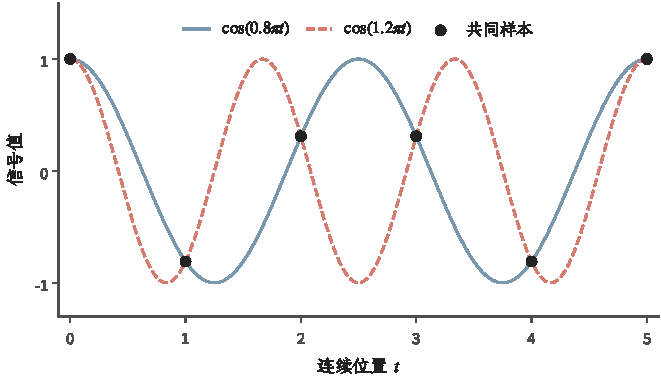
\includegraphics[width=\linewidth]{figures/01-mathematical-preliminaries/03-graphs-and-signals/matplotlib/dynamics/aliasing-curves.pdf}
  \caption{教学构造$f_1(t)=\cos(0.8\pi t)$与$f_2(t)=\cos(1.2\pi t)$。
  蓝色实线和红色虚线在整数时刻具有共同样本，深灰圆点标出这些观测。
  图只展示$[0,5]$，样本相同对所有整数成立；两条纯余弦是功率信号，
  不属于后文定理中的整轴平方可积信号类。}
  \label{fig:signal-aliasing-curves}
\end{figure}

任何确定性插值器对相同输入样本只能返回同一输出，因此不可能同时正确恢复这两条曲线。
学习模型可以凭训练分布猜测更常见的细节，但这种能力来自额外先验，
不是采样映射自己变成可逆。这里的余弦有有限平均功率而整轴能量无穷，
只用于展示歧义；后文将换到$L^2$带限空间，不能把此例当作那个空间中的反例。
对一般$L^2$等价类，点值采样本身还未定义，下一小节会先补齐代表元条件。

离散信号也可以丢弃位置。对正整数$M$保留每$M$项中的一项，
$y[n]=x[Mn]$，称为$M$倍\term{下采样}（downsampling）。
其DTFT满足
\begin{equation}
  Y(e^{\mathrm i\omega})=\frac1M\sum_{\ell=0}^{M-1}
  X\left(e^{\mathrm i(\omega+2\pi\ell)/M}\right).
  \label{eq:signal-analysis-downsampling-spectrum}
\end{equation}
对$x\in\ell_1$，按定义展开右侧并交换有限和与绝对收敛级数，
\begin{align*}
  \frac1M\sum_{\ell=0}^{M-1}X\left(e^{\mathrm i(\omega+2\pi\ell)/M}\right)
  &=\sum_{r\in\mathbb Z}x[r]e^{-\mathrm ir\omega/M}
    \left(\frac1M\sum_{\ell=0}^{M-1}e^{-2\pi\mathrm i\ell r/M}\right)\\
  &=\sum_{n\in\mathbb Z}x[Mn]e^{-\mathrm i\omega n}.
\end{align*}
括号内的单位根和只在$M\mid r$时为$1$，否则为$0$，故留下的恰为输出DTFT。
对$x\in\ell_2$，下采样满足$\sum_n|x[Mn]|^2\leq\sum_r|x[r]|^2$，
频域右侧的有限分支映射在$L^2$中也有界；
先对有限截断证明再取$L^2$极限，便得到同一公式的等价类解释。

输入模式$e^{\mathrm i\omega_0n}$变为$e^{\mathrm iM\omega_0n}$，
输入频率映到$M\omega_0\bmod2\pi$。
原频谱沿输出频率轴扩展$M$倍，超出主值区间的部分回绕，与其他分量相加。
所以“样本点变少”不只是频率曲线画得稀疏，而可能直接合并原来不同的频率。
连续采样的频谱复制也有类似现象，但必须在可读取点值的信号类上推导。

\subsection{信号约束下的恢复与预滤波}

排除歧义有两种不同做法：限制原信号本来就属于可恢复的类，或者先改变原信号，
使准备保留的部分适合新的采样间隔。前者讨论从原信号样本精确恢复，
后者讨论采样前删掉或压低哪些分量，恢复目标也随之改变。

\subsubsection{带限条件下的精确恢复}
\label{sec:signal-bandlimited-recovery}

带限用频率约束限制候选函数，而非只规定观察多长时间。
\begin{definition}[平方可积带限信号]
  \label{def:signal-analysis-bandlimited-space}
  设$\Omega_{\max}>0$、$f\in L^2(\mathbb R)$，其Plancherel意义的傅里叶变换为$F$。
  若$F(\Omega)=0$对几乎处处的$|\Omega|>\Omega_{\max}$成立，
  称$f$带限于$\Omega_{\max}$。
  所有这类函数组成\term{Paley--Wiener带限空间}。
\end{definition}
只观察一个有限时间窗口，不能推出窗口外为零，更不能推出高频为零。
带限才是下面用来排除混叠的信号类条件。

带限还使点值有规范含义。由$F\in L^2$及频谱支撑长度有限，
Cauchy--Schwarz不等式给出
\[
  \|F\|_1\leq\sqrt{2\Omega_{\max}}\,\|F\|_2<\infty.
\]
因此
\[
  f_{\mathrm c}(t)=\frac1{2\pi}\int_{-\Omega_{\max}}^{\Omega_{\max}}
  F(\Omega)e^{\mathrm i\Omega t}\,\mathrm d\Omega
\]
是$f$的连续代表元；连续性由以$|F|$为可积控制函数的控制收敛得到。
两个连续代表元若几乎处处相等，就处处相等，所以这种选择唯一。
以下仍记它为$f$，样本$f(nT_s)$都针对这个代表元，不针对随意改过点值的版本。

记采样角频率$\Omega_s=2\pi/T_s$，基带
$I_s=[-\pi/T_s,\pi/T_s]$。这里\term{基带}（baseband）指选定的一段基本频率区间。
将频谱副本按间隔$\Omega_s$相加，
\[
  P_F(\Omega)=\frac1{T_s}\sum_{k\in\mathbb Z}F(\Omega-k\Omega_s).
\]
由于$F$带限，在$I_s$上只有有限多个平移副本可能非零，故$P_F\in L^2(I_s)$，
并以$\Omega_s$为周期。
采用基$e^{-\mathrm i\Omega nT_s}$，其第$n$个傅里叶系数为
\begin{align*}
  \frac1{\Omega_s}\int_{I_s}P_F(\Omega)e^{\mathrm i\Omega nT_s}\,\mathrm d\Omega
  &=\frac1{2\pi}\int_{\mathbb R}F(\Omega)e^{\mathrm i\Omega nT_s}\,\mathrm d\Omega\\
  &=f(nT_s)=x[n].
\end{align*}
第一步令$u=\Omega-k\Omega_s$，各平移区间拼回实轴，
且$e^{\mathrm inT_sk\Omega_s}=e^{2\pi\mathrm ink}=1$；
第二步就是所选连续代表元的逆变换。
由周期Parseval关系，系数序列$x$属于$\ell_2$，故样本的频率表示
$X_s(\Omega)=\sum_n x[n]e^{-\mathrm i\Omega nT_s}$
在$L^2(I_s)$中有定义。它与$P_F$的全部系数相同，得到
\begin{equation}
  X_s(\Omega)=\frac1{T_s}\sum_{k\in\mathbb Z}F(\Omega-k\Omega_s).
  \label{eq:signal-analysis-spectral-replication}
\end{equation}
这也就是DTFT在$\omega=\Omega T_s$下的写法。
采样不是只保留一份原频谱，而是周期复制再叠加。
以上推导只用带限空间、傅里叶级数和积分，不需把采样写成Dirac脉冲列乘积；
若采用后者，则要另行建立广义函数的乘积与变换规则。

当$\Omega_s>2\Omega_{\max}$时，邻近副本不重叠，基带内只有中央副本。
当$\Omega_s<2\Omega_{\max}$时，允许频带与其平移副本在正测度区间重叠，
整个带限空间上的采样不再单射：可在频带内选择小区间$J$，
使$J$和$J+\Omega_s$都留在频带中且不相交；
在$J$上放任意非零$L^2$频谱，在$J+\Omega_s$上放其负平移，
两份周期复制相消，于是非零信号的全部样本为零。
临界$\Omega_s=2\Omega_{\max}$仅在端点相接，
零测端点不改变当前$L^2$等价类，不能把它与正测度重叠一概而论。

\begin{theorem}[带限信号的采样重构]
  \label{thm:signal-analysis-sampling}
  若$f$属于上述Paley--Wiener空间，频谱支撑包含于
  $[-\Omega_{\max},\Omega_{\max}]$，且$\Omega_s>2\Omega_{\max}$，
  则全部样本$f(nT_s)$唯一确定$f$，并有
  \begin{equation}
    f(t)=\sum_{n\in\mathbb Z}f(nT_s)
    \operatorname{sinc}\left(\frac{t-nT_s}{T_s}\right),
    \qquad \operatorname{sinc}(u)=\frac{\sin(\pi u)}{\pi u},
    \label{eq:signal-analysis-sinc-reconstruction}
  \end{equation}
  其中$\operatorname{sinc}(0)=1$。对称部分和在$L^2(\mathbb R)$中收敛，
  并对所选连续代表元在整条实轴上一致收敛。
\end{theorem}
\begin{proof}
  条件保证$F$的支撑严格落在$I_s$内，频谱复制式在该区间上给出$F=T_sX_s$。
  因此$F$相对于$e^{-\mathrm i\Omega nT_s}$的傅里叶系数是$T_sf(nT_s)$，
  部分和
  \[
    F_K(\Omega)=T_s\sum_{n=-K}^{K}f(nT_s)e^{-\mathrm i\Omega nT_s}
  \]
  在$L^2(I_s)$中趋于$F$。把$F_K$在$I_s$外取零，逆变换的有限和可移入积分外：
  \begin{align*}
    f_K(t)
    &=\sum_{n=-K}^{K}f(nT_s)\frac{T_s}{2\pi}
      \int_{-\pi/T_s}^{\pi/T_s}e^{\mathrm i\Omega(t-nT_s)}\,\mathrm d\Omega\\
    &=\sum_{n=-K}^{K}f(nT_s)
      \operatorname{sinc}\left(\frac{t-nT_s}{T_s}\right).
  \end{align*}
  对$t\neq nT_s$，指数积分是$2\sin(\pi(t-nT_s)/T_s)/(t-nT_s)$；
  当$t=nT_s$时，积分为区间长度$2\pi/T_s$，乘上$T_s/(2\pi)$后才等于$1$。
  这与$\operatorname{sinc}(0)=1$的连续延拓一致。
  Plancherel等式给出
  $\|f_K-f\|_2=(2\pi)^{-1/2}\|F_K-F\|_2\to0$，
  从而得到$L^2$重构。

  由于误差频谱仍支持在$I_s$内，逐点误差还满足
  \[
    \sup_{t\in\mathbb R}|f_K(t)-f(t)|
    \leq\frac1{2\pi}\|F_K-F\|_{L^1(I_s)}
    \leq\frac{\sqrt{|I_s|}}{2\pi}\|F_K-F\|_{L^2(I_s)}
    \longrightarrow0.
  \]
  这证明整轴一致收敛。所用关键是有限频谱支撑，
  不能把这项结论直接套到任意周期$L^2$函数的逐点傅里叶展开。

  若两条满足条件的信号样本相同，则频谱在$I_s$上的所有傅里叶系数相同。
  完备性使两频谱几乎处处相等，逆变换后得到同一$L^2$元素及同一连续代表元，
  因而恢复唯一。
\end{proof}

sinc在整数非零点为零、在原点为一，所以每个基函数在自己的样本位置给出系数，
在其他样本位置不作贡献。这解释了公式为何插值全部样本，
但仅核对这些点还不能证明样本之间等于原函数；后者依靠带限性与刚才的唯一性证明。
由基带Parseval还可得$\|f\|_2^2=T_s\sum_n|f(nT_s)|^2$，
说明在当前条件下，连续能量与离散样本能量只差采样间隔因子。

定理用严格不等号留下频率余量。同一证明可在当前$L^2$模型中按几乎处处意义延伸至
$\Omega_s=2\Omega_{\max}$，端点相接无碍。
若扩大到允许谱线的功率信号，临界点要另行处理：
$\sin(\Omega_{\max}t)$在$T_s=\pi/\Omega_{\max}$的全部样本为零，
但它不属于$L^2(\mathbb R)$，因此并不反驳此处结论。

定理使用全部双向无限样本，理想sinc也有无限支撑。
有限时长、噪声、未知带宽及非带限分量不会因公式而消失；
有限记录只能支持截断或其他有条件的近似重构，不能宣称享有同样的无误差保证。
把有限窗口外补零还会改变原信号，不能用这个人为边界代替带限假设。

\subsubsection{下采样条件下的抗混叠处理}

若原信号含有将在抽取后重叠的频率，就应在下采样前限制这些分量，
这种预处理称为\term{抗混叠滤波}（anti-aliasing filtering）。
对$M$倍下采样，理想低通将频率支持限制到$|\omega|<\pi/M$内，
使式~\eqref{eq:signal-analysis-downsampling-spectrum}中的频谱副本不混在一起。
这里恢复的目标是预滤波后的信号，不是已经被滤掉的全部原信号。
设计时把希望保留的频段称为通带（passband），把希望压低的频段称为
阻带（stopband）；这些名称描述对频率响应的要求，而不表示实际滤波器已经满足要求。

局部平均提供容易计算的平滑，却不自动满足理想低通条件。
长度$M$的均值核为$h[n]=1/M$（$0\leq n<M$），其余为零。
由有限几何级数，
\[
  H(e^{\mathrm i\omega})=\frac1M\sum_{n=0}^{M-1}e^{-\mathrm i\omega n}
  =\frac1M\frac{1-e^{-\mathrm iM\omega}}{1-e^{-\mathrm i\omega}},
\]
再从分子分母各提出中间相位因子，得到
\begin{equation}
  H(e^{\mathrm i\omega})=
  \frac1M e^{-\mathrm i\omega(M-1)/2}
  \frac{\sin(M\omega/2)}{\sin(\omega/2)}.
  \label{eq:signal-analysis-moving-average-response}
\end{equation}
当$\omega\in2\pi\mathbb Z$出现$0/0$时，按原有限和取连续值$1$。
该响应有衰减和零点，却不能将一整段阻带频率都消去。
当$M\geq3$时，在主频率区间$[-\pi,\pi]$内还可看到主峰以外的小峰，
称为旁瓣（sidelobes），它们直接显示了高频残留。
相位因子反映以当前及过去样本实现均值时的时间对齐；
按窗口输出的平均池化（average pooling）可看成这种滤波后抽取。
具体地，对同一长度$M$窗口，平均池化和最大池化（max pooling）分别为
\[
 \begin{aligned}
  p_{\mathrm{avg}}[m]&=\frac1M\sum_{r=0}^{M-1}x[Mm+r],\\
  p_{\mathrm{max}}[m]&=\max_{0\leq r<M}x[Mm+r].
 \end{aligned}
\]
若$y=x*h$使用前述因果均值核，则$p_{\mathrm{avg}}[m]=y[Mm+M-1]$，
窗口起点与卷积输出时刻之间有明确的索引偏移。
最大池化不满足线性叠加：窗口$(1,0)$和$(0,1)$的最大值都为$1$，
相加后的窗口$(1,1)$最大值仍为$1$，并非两个输出之和$2$。
因此不能用一个固定线性频率响应完整描述最大池化。

同一两频输入可以比较直接抽取、理想低通和均值预滤波：
\[
  x[n]=\cos(0.2\pi n)+\cos(0.8\pi n).
\]
直接二倍抽取得到$x[2m]=2\cos(0.4\pi m)$，
因为$1.6\pi$与$-0.4\pi$在整数位置对应相同余弦。
若先理想低通完全删除$0.8\pi$分量，输出则为$\cos(0.4\pi m)$。
若仅用$h=(1/2,1/2)$，恒等式
\[
  \frac{\cos(\omega n)+\cos(\omega(n-1))}{2}
  =\cos(\omega/2)\cos(\omega n-\omega/2)
\]
表明抽取后为
\[
  \cos(0.1\pi)\cos(0.4\pi m-0.1\pi)
  +\cos(0.4\pi)\cos(1.6\pi m-0.4\pi).
\]
第二项仍折回低频，只是幅度降低并发生相位偏移。
均值滤波在原高频处的残留幅度为
\[
 |H(e^{\mathrm i0.8\pi})|=\cos(0.4\pi)>0,
\]
所以它没有清除这个高频。
这些纯余弦用于按模式计算频率响应，是功率信号算例，不把它们误放进前述$L^2$恢复定理。
“已经平滑”与“满足无混叠带限条件”因此不是同一个保证。

有限长度核的频率响应是有限个复指数的线性组合，也称三角多项式。
若在一整段频率上精确为零，就会迫使对应
多项式恒为零。因此，非零有限核不能实现从完全保留突变到完全抑制的理想低通。
实际设计通常允许通带与阻带之间留出一段缓变的过渡带（transition band）。
通带误差衡量保留频段的响应偏离目标多少，阻带衰减衡量抑制频段还剩多大幅度；
它们需要与过渡带宽度、延迟及计算量一起规定。
滤波后剩余的混叠是设计误差的一部分，不能因用了低通名称就忽略。
如果响应在某频段为零，该频段进入映射零空间；接近零的响应虽可能形式可逆，
反演却会放大噪声。第~\ref{chap:linear-algebra-and-matrix-analysis}章
“线性空间”中的零空间与小奇异值分析在这里仍然适用：
前者说明哪些输入区别完全不可见，后者说明哪些区别虽可见却难以稳定恢复。

\section{本章小结}
\label{sec:signal-analysis-summary}

分析信号先要确定在哪里取值、每个位置有几个通道，以及首尾如何连接。
有限记录不等于有限支撑，通道数不等于时间长度，周期延拓也不等于原过程周期。
内积规定比较口径，范数与能量衡量累计大小，平均功率则适合长期持续的信号；
改变通道权重或观察窗口，比较的对象也随之改变。

脉冲、傅里叶和多项式表示从不同方向描述同一信号。
完整有限DFT及满足次数条件的插值可以无损恢复坐标，无穷傅里叶展开则需要说明
积分、均方或逐点意义。幅度不包含全部位置信息，Parseval中的尺度因子来自归一化，
截断系数才引入相应的表示误差。

平移、反转、幅值及时间缩放改变的是不同属性。
线性与平移不变使有限脉冲响应组合为卷积，无穷输入还需有界性或可积条件。
时变核可以线性却不只依赖滞后，输入门控则通常破坏叠加；
多通道矩阵核还须分清时间汇总与通道混合。
相关按原模板方向比较局部片段，不能只凭实现名称把它与卷积混同。
FFT、Toom--Cook和Winograd用不同表示减少同一目标的计算，
核方向、边界、输出范围及数值条件仍由目标决定。

采样最后改变了可用信息。不同信号可能具有同一样本，坐标可逆和计算快速都不能补回
已经消失的区别。带限有限能量类、规范连续代表元及足够密的无限样本共同给出sinc恢复；
有限记录和功率信号需要各自核对边界。抗混叠预滤波可以控制即将重叠的频率，
却也改变待恢复的目标。下一章把规则索引推广为一般图：连接关系决定哪些位置可以
比较与传播，图上的谱则提供相应的变化坐标。后面的随机变量部分描述观测中的不确定性；
第~\ref{chap:dynamical-systems-and-state-estimation}章再增加内部状态，解释响应核怎样从演化规律产生。
本章保留的输入输出视角则继续用于判断这些响应怎样作用于信号。

\chapter{图的表示与计算}
\label{chap:graph-theory}

把四个变量之间的局部约束画成一张图以后，能否从一个变量走到另一个变量？
哪些变量可以分开处理，哪些选择能获得最优性证书？若在每个顶点放一个数，
邻域汇总又会保留或抹去什么？这些问题共享连接结构，却需要不同的计算规则。
本章把图本身作为研究对象，利用已有的集合、逻辑与线性代数工具，建立路径查询、
结构分解、离散选择及图上函数的运算。后续第~\ref{chap:causal-inference}章再说明
图怎样表达生成机制，以及什么条件下图分离能够推出概率独立。本章的图判据与局部
计算先独立成立；局部传播是否精确，还须检查函数分解与运算规则。

继续使用第~\ref{chap:combinatorics}章的四个二值变量
\[
  z_i\in\{0,1\},\qquad i\in V=\{1,2,3,4\}.
\]
式~\eqref{eq:comb-running-cnf}的前两个子句共同涉及\(z_1,z_2\)，
第三个子句涉及\(z_1,z_3\)，三变量子句
\(\neg z_4\lor z_2\lor z_3\)则同时涉及\(z_2,z_3,z_4\)。
把共同出现的每一对变量连接，得到
\begin{equation}
  E=\bigl\{\{1,2\},\{1,3\},\{2,3\},\{2,4\},\{3,4\}\bigr\}.
  \label{eq:graph-theory-running-edges}
\end{equation}
图~\ref{fig:graph-theory-running-graph}中，左右两个三角形共享顶点\(2,3\)。
固定这两个变量以后，左右两侧的局部计算可以分别进行；但三元子句仍须保留，
三条两两连接并没有把它变成三个等价的二元约束。

\begin{figure}[htbp]
  \centering
  \begin{tikzpicture}[text=FigureInk,
    vertex/.style={circle,draw=FigureStroke,fill=FigureYellowFill,line width=1pt,
      minimum size=8mm,inner sep=0pt,font=\figurefont\footnotesize},
    edge/.style={draw=FigureStroke,line width=1.1pt}
  ]
    \node[vertex] (x2) at (0,1.15) {\(z_2\)};
    \node[vertex] (x3) at (0,-1.15) {\(z_3\)};
    \node[vertex] (x1) at (-2.1,0) {\(z_1\)};
    \node[vertex] (x4) at (2.1,0) {\(z_4\)};
    \draw[edge] (x1)--(x2);
    \draw[edge] (x1)--(x3);
    \draw[edge] (x2)--(x3);
    \draw[edge] (x2)--(x4);
    \draw[edge] (x3)--(x4);
  \end{tikzpicture}
  \caption{由四变量约束的作用域导出的关系图。边表示两个变量共同出现在至少一个
  约束中；共享顶点集合\(\{2,3\}\)连接左右两侧。图没有记录约束的具体真值表，
  也没有预先指定边长、容量或相似度。}
  \label{fig:graph-theory-running-graph}
\end{figure}

本章先确定图记录的对象，再沿路径检索关系。由路径得到的分隔接口，可以组织局部块；
结构抽取和消元则说明改写图时保留什么、增加什么。给定结构以后，路径、流量、树、
匹配和标签的最优选择各有自己的目标与条件。图上函数的变换还要区分两种定义域：
给每个顶点一个数，与给全部变量的一次完整赋值一个数，所需运算并不相同。
这种区分连接图谱滤波与局部精确查询，也说明前章规则信号中的变换与卷积
推广到一般连接结构时，需要重新选择哪些对象与运算。

\section{图的对象与表示}
\label{sec:graph-theory-objects-representations}

画一条线之前，需要说明它记录的是对称关系、有方向的作用，还是某个多变量函数的
作用域。确定对象以后，邻接表与矩阵只是同一结构的不同存储方式；改变顶点编号
也不应改变结构本身。这里固定这些约定，路径、优化和传播再分别使用它们。

\subsection{局部关系的对象与作用域}
\label{sec:graph-theory-local-relations}

\subsubsection{二元关系的图表示}
\label{sec:graph-theory-binary-relations}

若只需记录哪些对象直接相关，可以让每个对象对应一个顶点，让一对对象的关系对应
一条边。\term{无向图}（undirected graph）是
\(\mathcal G=(V,E)\)，其中\(V\)是有限顶点集合，\(E\)是不同顶点的无序对集合。
本章默认没有自环，也没有同一对顶点之间的平行边；允许这些情形时，要另外保存
边的身份及重数，不能继续把边集理解成普通无序对集合。

若\(\{i,j\}\in E\)，称\(i,j\)相邻，二者互为邻居。
顶点\(i\)的\term{邻域}（neighborhood）是它的全部邻居，
\term{度}（degree）是邻居的数量：
\[
  N(i)=\{j\in V:\{i,j\}\in E\},\qquad d_i=|N(i)|.
\]
贯穿图中\(N(2)=\{1,3,4\}\)、\(d_2=3\)，而
\(N(1)=\{2,3\}\)、\(d_1=2\)。度只统计直接连接，不统计经过其他顶点能够到达的对象。

关系具有方向时，使用\term{有向图}（directed graph）
\(\mathcal G=(V,A)\)，其中\(A\subseteq V\times V\)是有序对的集合，
并仍排除\((i,i)\)。弧\((i,j)\)写作\(i\to j\)，不自动包含反向弧。
入邻域\(N^-(j)=\{i:i\to j\}\)与出邻域\(N^+(j)=\{i:j\to i\}\)
分别记录指向本点和从本点指出的对象；它们的大小称为
\term{入度}（in-degree）和\term{出度}（out-degree）。
有向图中也常把入邻居称为父节点，把出邻居称为子节点。这些名称只说明连接方向；
一般有向边可以表示计算依赖或允许通行的方向，不能只凭箭头赋予因果意义。

在结构边上还可以指定\term{权重}（weight），即每条边附带的数值。
无向权重满足\(w_{i,j}=w_{j,i}\)，有向权重允许方向不同。
有向与无向描述方向，加权与无权描述是否附带数值，是能够组合的两个属性。
边长越大表示经过它的成本越高，容量越大表示允许通过的总量越多，
相似度越大则通常表示两端越接近；同一个数字不能未经转换同时充当这三种量。

结构存在也不等于权重非零。本章允许零权结构边，另把无向非负权图中的
\[
  E_+=\{\{i,j\}\in E:w_{i,j}>0\}
\]
称为\term{正权支撑}（positive-weight support）。
例如两顶点之间存在一条权重为零的边，结构上仍相邻，但在线性加权汇总中互不贡献。
因此后面的谱与扩散结论使用支撑图\(\mathcal G_+=(V,E_+)\)，
而结构路径查询是否使用零权边，要由查询规则另行决定。

只研究部分对象时，不能无声改掉它们之间的关系。给定\(U\subseteq V\)，
保留\(U\)及原图中两端都属于\(U\)的全部边或弧，所得图称为
\term{诱导子图}（induced subgraph），记作\(\mathcal G[U]\)。
贯穿图在\(\{1,2,3\}\)上的诱导子图必须保留三条边；只留下\(1-2-3\)
是一个子图，却不是该顶点集上的诱导子图。

\subsubsection{高阶关系的因子表示}
\label{sec:graph-theory-higher-order-scopes}

三元子句\(\neg z_4\lor z_2\lor z_3\)要求同时查看三个变量。
这种局部函数称为因子（factor），它依赖的变量集合称为作用域（scope）。
要保留“共同属于同一个因子”的信息，可以使用\term{超图}（hypergraph）：
每条超边是一个顶点子集，不限于两个顶点；超边\(\{2,3,4\}\)在这里记录三元作用域。
函数值仍须另外保存，超边本身也不是约束真值表。

另一种表示把变量和因子分成两组，只在变量属于因子作用域时连边。
两组顶点内部都没有边的图称为\term{二部图}（bipartite graph）；
这样得到的因子图（factor graph）用方形顶点保存因子的身份，用圆形顶点保存变量。
若只保留变量，并把每个因子作用域内的变量两两相连，得到
\term{原始关系图}（primal graph），也简称原始图。
贯穿图正是按这条规则由原子句得到的。

图~\ref{fig:graph-theory-factor-scope}比较两种表示。一个三元因子和三个二元因子
可以产生同一个三角形原始图，但它们的函数族一般不同。
例如二值三元约束“恰有偶数个变量等于\(1\)”允许
\(000,011,101,110\)。每一对变量的四种取值都在某个允许配置中出现；
若只保留这三个二元允许关系，它们便不再排除任何配置，错误地允许了\(001\)。
两两关系无法恢复被丢失的三元相容条件。

\begin{figure}[htbp]
  \centering
  \begingroup
% Local styles; callers keep this input inside a group.
\tikzset{
  reader vertex/.style={circle,draw=FigureStroke,fill=white,line width=1pt,
    minimum size=7mm,inner sep=0pt,font=\figurefont\footnotesize,text=FigureInk},
  reader factor/.style={rectangle,draw=FigureStroke,fill=FigureYellowFill,
    line width=1pt,minimum size=8mm,inner sep=2pt,font=\figurefont\footnotesize},
  reader edge/.style={draw=FigureStroke,line width=1.1pt},
  reader arrow/.style={reader edge,-{Stealth[length=2.2mm,width=1.4mm]}},
  reader label/.style={font=\figurefont\footnotesize,text=FigureInk},
  reader note/.style={reader label,fill=white,inner sep=1pt},
  reader highlight/.style={draw=FigureYellow,line width=1.1pt},
  reader auxiliary/.style={draw=FigureMuted,line width=0.6pt,dashed}
}

\begin{tikzpicture}[text=FigureInk]
  \node[reader label] at (0,1.35) {(a) 三元因子};
  \node[reader factor] (f) at (0,0) {\(\phi_{2,3,4}\)};
  \node[reader vertex] (a) at (-1.35,0) {\(z_2\)};
  \node[reader vertex] (b) at (0,-1.05) {\(z_3\)};
  \node[reader vertex] (c) at (1.35,0) {\(z_4\)};
  \draw[reader edge] (a)--(f)--(c);
  \draw[reader edge] (b)--(f);
  \node[reader label] at (4.8,1.35) {(b) 原始关系图};
  \node[reader vertex] (x) at (3.45,0) {\(z_2\)};
  \node[reader vertex] (y) at (4.8,-1.05) {\(z_3\)};
  \node[reader vertex] (z) at (6.15,0) {\(z_4\)};
  \draw[reader edge] (x)--(y)--(z)--(x);
\end{tikzpicture}
\endgroup

  \caption{三元因子与原始关系图。左侧方框是同一个依赖\(z_2,z_3,z_4\)的函数，
  连线表示作用域归属；右侧只保留变量共同出现的两两关系。右侧三条边不是把三元
  函数分解成三个二元函数的等价变换，也不能恢复原函数的数值。}
  \label{fig:graph-theory-factor-scope}
\end{figure}

\subsection{图关系的矩阵表示}
\label{sec:graph-theory-matrix-representations}

遍历要快速取出邻居，线性汇总要快速相乘，边差分还要逐边保留端点。
邻接表、邻接矩阵和关联矩阵分别直接支持这三种操作。
邻接表为每个顶点存实际邻居及其边属性，空间为\(O(|V|+|E|)\)；
无向边在两个端点各存一次只改变常数。稠密邻接矩阵则为每一对顶点预留一个位置。

固定顶点次序\(1,\ldots,n\)，\term{邻接矩阵}（adjacency matrix）
\(\bm A\in\mathbb R^{n\times n}\)的条目为
\[
  a_{i,j}=
  \begin{cases}
    w_{i,j},&\{i,j\}\in E\quad\text{或}\quad(i,j)\in A,\\
    0,&\text{其他情形}.
  \end{cases}
\]
无权边取权重\(1\)。有向情形约定行是起点、列是终点，因此
\((\bm A\bm f)_i=\sum_{j\in N^+(i)}w_{i,j}f_j\)
汇总出邻居的值；若要把每个起点的值沿出弧发送到终点，应使用
\(\bm A^\top\bm f\)。无向图中矩阵对称，两种读法才重合。
贯穿图对应
\begin{equation}
  \bm A=
  \begin{bmatrix}
    0&1&1&0\\
    1&0&1&1\\
    1&1&0&1\\
    0&1&1&0
  \end{bmatrix}.
  \label{eq:graph-theory-running-adjacency}
\end{equation}
例如\(\bm f=(1,2,3,4)^\top\)给出
\(\bm A\bm f=(5,8,7,5)^\top\)。这是顶点值的线性汇总，
不等于在全部变量配置上求和；后者还需要明确局部因子。
允许零权边时，矩阵条目\(0\)不能区分无边与零权边，必须另存边集或结构掩码
\(m_{i,j}=\mathbb I\{\text{存在相应结构边}\}\)。

要计算每条边两端的差，给每条无向边任选临时方向，构造
\term{关联矩阵}（incidence matrix）
\(\bm B\in\mathbb R^{|V|\times|E|}\)。
边\(e:i\to j\)对应列在\(i\)处取\(1\)，在\(j\)处取\(-1\)，其余为零。
于是\((\bm B^\top\bm f)_e=f_i-f_j\)。
若\(\bm W_E=\operatorname{diag}(w_e:e\in E)\)，
\(\bm B\bm W_E\bm B^\top\)先求边差、按权缩放，再汇总回顶点。
反转某些临时方向相当于\(\bm B'=\bm B\bm R\)，其中
\(\bm R\)为对角元取\(\pm1\)的对角矩阵。
由于\(\bm R\bm W_E\bm R=\bm W_E\)，这个无向加权差分算子不随临时方向改变。
这并没有消除真正有向图中的方向，二者不能混用。

\subsection{顶点重编号下的结构同一性}
\label{sec:graph-theory-graph-isomorphism}

矩阵的位置依赖编号，图的连接关系却不应依赖编号。
两图\(\mathcal G=(V,E)\)、\(\mathcal G'=(V',E')\)若存在双射
\(\rho:V\to V'\)，使
\[
  \{i,j\}\in E
  \quad\Longleftrightarrow\quad
  \{\rho(i),\rho(j)\}\in E',
\]
就称为\term{同构}（isomorphic）：忽略顶点名称后，两图的连接完全相同。
有向图要保有序弧，加权图还要保对应权重，带属性图则须说明哪些属性也要求保持。
设置换矩阵满足\((\bm P\bm f)_{\rho(i)}=f_i\)，重编号对应
\begin{equation}
  \bm A'=\bm P\bm A\bm P^\top.
  \label{eq:graph-theory-adjacency-relabel}
\end{equation}
这是置换共轭，只挪动坐标位置，不把两个顶点的值混合。
第~\ref{chap:matrix-analysis}章的一般相似变换允许混合坐标，
所以不能把任意换基都解释成图重编号。

数值矩阵单独判同构，还要求它能恢复结构边。
无权图或所有结构边权非零时，式~\eqref{eq:graph-theory-adjacency-relabel}
给出矩阵判据；允许零权结构边时，还须验证
\(\bm M'=\bm P\bm M\bm P^\top\)。
两顶点空图与两顶点零权单边图都可有\(\bm A=\bm0\)，但前者不相邻、后者相邻。

同构必有相同邻接谱，因为置换共轭是相似变换；逆命题不成立。
例如四叶星图\(K_{1,4}\)与“四环加一个孤立顶点”都有邻接特征值
\(2,-2,0,0,0\)。前者的非零特征值来自中心与四个叶顶点的汇总，
后者的四环特征值为\(2,0,0,-2\)，再加孤立点的零值。
一图连通、另一图不连通，故不同构。这里比较的是邻接谱；
后文不同算子的谱也必须指明算子，不能只说“两个图的频率相同”。
图上顶点函数随编号怎样变化，将在第~\ref{sec:graph-theory-vertex-functions}节
用这里的置换关系检验。

\section{图上的关系、路径和遍历}
\label{sec:graph-theory-paths-traversal}

顶点不相邻，并不表示二者毫无联系：关系可以经其他顶点延伸。
本节从一条边扩展到一条路径，再区分“存在某条路径”“所有路径都被阻断”
和“找到代价最小的路径”。遍历负责检索这些对象；加权最优选择所需的额外条件，
在第~\ref{sec:graph-theory-shortest-paths}节集中处理。

\subsection{两点之间的关系}

贯穿图中\(1,2\)直接相邻，\(1,4\)不相邻，但可以通过\(2\)连接。
有向图的直接关系还要看方向：\(i\to j\)允许一步从\(i\)到\(j\)，
不能据此反向通行。两点之间的权重只修饰已声明的关系。
若边长为\(5\)，经过这条边付出成本\(5\)；若容量为\(5\)，它限制的是总通过量；
若相似度为\(5\)，它通常鼓励两端数值接近，而不是要求路径绕开该边。

零边长可以表示免费通行，零容量表示不能承载正流量，零相似度则不贡献加权差分。
三者都不自动删除结构边。因此“这两个顶点之间能否走一步”应查边集及方向，
不能只检查某个数值矩阵的条目是否大于零。

\subsection{图上的路径与环}

\subsubsection{行走、简单路径与环}

把相邻关系首尾连接得到行走，也称\term{游走}（walk）：它是顶点序列
\(v_0,v_1,\ldots,v_k\)，每对相邻项之间都有边，允许重复顶点和边。
若顶点两两不同，就称为简单\term{路径}（path），本章无修饰的“路径”
默认指简单路径。边数长度为\(k\)，单个顶点构成长度为零的路径。
无向简单图中的\term{环}（cycle）是长度\(k\geq3\)的闭行走，
其中\(v_0=v_k\)，而\(v_0,\ldots,v_{k-1}\)两两不同。
例如贯穿图的\(1,2,3,1,2\)是行走，\(1,2,4\)是路径，\(1,2,3,1\)是环。

有向行走与\term{有向路径}（directed path）的每一步都必须沿弧方向。
\term{有向环}（directed cycle）除首尾外顶点互异，并且闭行走的每一步都顺着弧。
无自环有向图的环可短至两条弧：\(i\to j\to i\)已经成环；
无向图中沿同一条边走去再返回却不是环。不含有向环的图称为
\term{有向无环图}（directed acyclic graph, DAG）。
这里的“无环”不要求忽略方向后的图也无环，例如
\(1\to2\)、\(1\to3\)、\(2\to3\)构成DAG，但底层无向图是三角形。

邻接矩阵的幂可以检索行走，却不会替我们排除重复顶点。
对无权图，\((\bm A^k)_{i,j}\)等于从\(i\)到\(j\)长度为\(k\)的行走数。
当\(k=0\)时，\(\bm A^0=\bm I\)记录留在原点的零步行走；归纳地，
\[
  (\bm A^{k+1})_{i,j}=\sum_\ell(\bm A^k)_{i,\ell}a_{\ell,j}
\]
按倒数第二个顶点\(\ell\)分类，每个长度\(k+1\)的行走被计数恰好一次。
有向图沿行起点、列终点的约定使用同一证明。带权时则有
\[
  (\bm A^k)_{i,j}
  =\sum_{i=v_0\to v_1\to\cdots\to v_k=j}
    \prod_{r=1}^{k}w_{v_{r-1},v_r},
\]
无向边可向任一方向行走。这里得到的是权重乘积之和，不是行走条数，也不是边长之和。
将加法、乘法改成布尔运算或最小加法，会得到可达性或固定步数的最低成本，
但那已经换了矩阵运算规则。

\subsubsection{条件集合下的活跃路径}
\label{sec:graph-theory-active-paths}

沿箭头可达用于描述依赖方向；另一类查询还要指定顶点集合\(S\)，检查忽略方向后
连接两端的路径是否满足特定的通过规则。这里的\(S\)只是图查询的输入，不必先为
顶点指定随机变量。若从\(v\)沿长度至少为一的有向路径到达\(w\)，称\(w\)为
\(v\)的\term{后代}（descendant），\(v\)为\(w\)的\term{祖先}（ancestor）；
这两个名称都不包括顶点自身。

\begin{definition}[活跃路径与d-分离的图判据]
  \label{def:graph-theory-d-separation}
  设\(\mathcal G\)为DAG。底层路径上的内部顶点\(c\)若在该路径上呈现
  \(a\to c\leftarrow b\)，称为碰撞点，否则为非碰撞点。
  给定不含路径端点的顶点集合\(S\)，该路径\term{活跃}（active），当且仅当
  每个非碰撞内部顶点都不在\(S\)中，且每个碰撞点自身或某个后代属于\(S\)。

  对两两不交的顶点集合\(A,B,S\)，其中\(A,B\)非空，若连接\(A\)与\(B\)的
  每条底层路径都不活跃，称\(A,B\)被\(S\)\term{d-分离}（d-separated），记为
  \(A\perp_{\mathcal G}B\mid S\)；否则称为d-连接。
\end{definition}

“碰撞”是相对于当前路径两条相邻弧的角色，同一顶点在另一条路径上可能不是碰撞点。
路径是否活跃由箭头与\(S\)共同决定，并不等于能否沿箭头从起点走到终点。

考虑\(a\to c\leftarrow b\)和\(c\to d\)。
底层路径\(a-c-b\)在\(S=\varnothing\)时不活跃，因为碰撞点\(c\)没有被条件打开；
在\(S=\{c\}\)或\(S=\{d\}\)时活跃。后一个条件点甚至不在路径上，
却通过“碰撞点有后代被给定”的规则影响路径。
相反，在链\(a\to c\to b\)和分叉\(a\leftarrow c\to b\)上，
\(c\)都是非碰撞点，加入条件\(c\)会阻断路径。
这些都是图判据，不是对任意数值模型自动成立的概率断言。

\begin{figure}[htbp]
  \centering
  \begingroup
\begin{tikzpicture}[x=1mm,y=1mm,text=FigureInk,
  font=\figurefont\footnotesize,
  vertex/.style={circle,draw=FigureStroke,fill=white,line width=.9pt,
    minimum size=6mm,inner sep=0pt},
  given/.style={vertex,fill=FigureYellowFill,double=FigureYellowFill,
    double distance=1pt},
  edge/.style={draw=FigureStroke,line width=1pt,
    -{Stealth[length=1.8mm,width=1.2mm]}},
  note/.style={inner sep=0pt,fill=none}
]
  \path[use as bounding box] (0,0) rectangle (112,47);
  \foreach \x/\condition/\verdict in {
    16/{S=\varnothing}/{不活跃},
    56/{S=\{c\}}/{活跃},
    96/{S=\{d\}}/{活跃}} {
    \node[note] at (\x,43) {\(\condition\)};
    \node[vertex] (a\x) at (\x-12,30) {\(a\)};
    \node[vertex] (b\x) at (\x+12,30) {\(b\)};
    \node[note] at (\x,3) {\verdict};
  }
  \node[vertex] (c16) at (16,30) {\(c\)};
  \node[vertex] (d16) at (16,14) {\(d\)};
  \node[given] (c56) at (56,30) {\(c\)};
  \node[vertex] (d56) at (56,14) {\(d\)};
  \node[vertex] (c96) at (96,30) {\(c\)};
  \node[given] (d96) at (96,14) {\(d\)};
  \foreach \x in {16,56,96} {
    \draw[edge] (a\x) -- (c\x);
    \draw[edge] (b\x) -- (c\x);
    \draw[edge] (c\x) -- (d\x);
  }
\end{tikzpicture}
\endgroup

  \caption{同一底层路径\(a-c-b\)在三个条件集下的活跃性。箭头及顶点没有改变；
  空条件集未打开碰撞点，给定碰撞点\(c\)或其后代\(d\)都会打开它。
  双圈表示被给定的顶点，底部文字给出判定。活跃性不是沿箭头从\(a\)走到\(b\)
  的可达性，也不是简单删除条件顶点后的连通性。}
  \label{fig:graph-theory-active-paths}
\end{figure}

一条路径被阻断还不等于两端被分离，因为另一条路径可能仍活跃。
第~\ref{sec:graph-theory-conditional-separation}节将从单路径规则转向全部路径的查询。

\subsubsection{路径代价与最短路径}

若边的任务是记录长度或代价，记作\(\ell_{i,j}\)，以免与相似度混淆。
从\(s\)到\(t\)的路径\(P=(v_0=s,\ldots,v_k=t)\)的代价为
\[
  \ell(P)=\sum_{r=1}^{k}\ell_{v_{r-1},v_r}.
\]
最短路径选择使此和最小的路径。所有边长均为\(1\)时，它等于最少边数；
一般边长下则不等价。例如\(s-t\)长\(5\)，而\(s-u\)、\(u-t\)各长\(1\)，
两步路径比一步路径更短。

还须明确是否允许重复经过顶点。有限图只有有限条简单路径，因此只要可达，
简单路径代价就有最小值；允许行走时，候选数可以无限。
若可从\(s\)到达一个负代价闭行走，并从那里继续到\(t\)，反复经过它能使代价任意小。
此时行走代价下确界是\(-\infty\)，却不能说存在一条长度为\(-\infty\)的简单路径。
有向图的负闭行走必包含负有向环；无向负边仅往返一次就产生负闭行走，
即使它不在任何无向简单环上。无此负闭行走影响时，可以删去非负闭合段而不增加代价，
行走问题才与简单路径问题一致。不可达、负环及距离递推的统一约定稍后给出。

\subsection{图上的可达与连通}

\subsubsection{无向图的可达与连通}

若两点之间存在路径，就称它们互相可达。把可达顶点归在一起，得到
连通分量：每个分量内部任意两点可达，不同分量之间没有路径。
允许长度为零的路径使每个顶点与自身可达；反向路径给出对称性，
拼接两条路径并删去重复段给出传递性，故这些分量确实构成顶点集合的唯一划分。
只有一个分量的非空无向图称为\term{连通}（connected）。

贯穿图连通，删除\(\{1,2\}\)仍连通，因为\(1-3-2\)替代了原有边。
删除一个环上的边只破坏该环，不一定破坏连通；是否断开应检查有没有替代路径，
而非只数局部少了几条边。

\subsubsection{有向图的可达与连通}

有向可达要求存在顺着弧的路径，所以不再对称。
本章把通过正长度有向路径到达\(j\)的其他顶点称为\(j\)的祖先，
把从\(j\)通过正长度有向路径到达的其他顶点称为后代，二者均不含\(j\)自身。
一般有环图中两个不同顶点可以互为祖先，DAG中则不可能。
后文的祖先闭包会显式把起始集合本身加入，不借助这一措辞猜测。

若任意有序顶点对\(i,j\)间都有从\(i\)到\(j\)的有向路径，图称为
\term{强连通}（strongly connected）；互相可达的极大顶点集合称为强连通分量。
忽略弧方向后连通，则称为\term{弱连通}（weakly connected）。
强连通蕴含弱连通，但链\(1\to2\to3\)仅弱连通：
\(1\)可达\(3\)，\(3\)不能返回\(1\)，三个强连通分量各含一个顶点。
“两个点属于同一弱连通分量”并没有回答它们能否互相传递。

\subsubsection{树与森林的连通结构}

连通且无环的无向图称为\term{树}（tree），若干互不相连的树组成森林。
树的关键不是画面向外分叉，而是两点间没有第二条路径。
这让一个局部结果沿唯一接口传递，不会从另一条路重复返回。

\begin{theorem}[树的等价刻画]
  \label{thm:graph-theory-tree-characterizations}
  对含\(n\geq1\)个顶点的有限无向简单图，以下三条等价：
  \begin{enumerate}
    \item 图连通且无环；
    \item 任意两点之间恰有一条简单路径；
    \item 图连通，并且恰有\(n-1\)条边。
  \end{enumerate}
\end{theorem}

\begin{proof}
连通性保证至少一条路径；若有两条不同路径，沿二者从首次分开处到再次会合处
得到一个环，故无环时路径唯一。反过来，路径唯一包含连通性；
若有环，环上相邻顶点间既有该边，又有沿环另一侧的路径，与唯一性矛盾。

单顶点树有零条边。至少两个顶点的有限树必有度为\(1\)的叶顶点：
取最长简单路径，它的端点若有路径外邻居，可以延长路径；
若与路径上的非相邻顶点相连，则形成环。因此端点只有一个邻居。
删除叶顶点及其边后，余图仍连通且无环，归纳得原树边数为
\((n-1)-1+1=n-1\)。树中每条边又是其两端的唯一路径，删去该边必使两端断开。

最后，设图连通且有\(n-1\)条边。从一个顶点开始，每次加入一条连接已加入顶点
与未加入顶点的边。只要尚有顶点未加入，连通性就保证有这样的边。
每次只接入一个新顶点不会成环，重复\(n-1\)次便得到覆盖全部顶点的树。
这已经用完原图的\(n-1\)条边，故原图就是这棵树，也无环。
\end{proof}

只知道边数为\(n-1\)不够：三角形加一个孤立点有四个顶点、三条边，却不是树。
从一般连通图抽出一棵覆盖全部顶点的树，需要明确保留连接而舍弃其他边，
这将在第~\ref{sec:graph-theory-spanning-skeleton}节讨论。

\subsection{图上的遍历与次序}

\subsubsection{广度遍历与分层检索}
\label{sec:graph-theory-bfs}

要列出从\(s\)能到达的顶点，可以先查一跳邻居，再查两跳邻居。
\term{广度优先搜索}（breadth-first search, BFS）用先进先出队列维持这个次序。
初始化时标记\(s\)，置层数\(d(s)=0\)，将它入队。每次取出队首\(u\)，
检查它的邻居；有向图只检查出邻居。遇到尚未标记的\(v\)，立即标记并入队，
置\(d(v)=d(u)+1\)，同时记录父指针\(p(v)=u\)。
标记发生在入队时，防止两个已发现顶点把同一个邻居重复入队。

每个顶点最多入队一次，每条边或弧最多检查常数次，邻接表实现的时间为
\(O(|V|+|E|)\)\scite{math-cormen2022algorithms}
每个非起点的父指针指向较早发现的顶点，所以不会成环；
沿父指针回溯便能恢复从起点到它的发现路径。父边在可达集合上构成搜索树，
而不包含原图的全部边。

无权最短路性质由队列分层保证。归纳假设更早层都已经得到正确距离；
处理第\(k\)层时，新发现的邻居有一条长度\(k+1\)的路径。
若它存在更短路径，该路径的倒数第二个顶点应在更早层，并会更早发现它，矛盾。
因此首次记录的层数就是最少边数。贯穿图从\(1\)出发的层为
\(\{1\},\{2,3\},\{4\}\)，顶点\(4\)的父亲可以是\(2\)或\(3\)，但距离同为\(2\)。
不同父树不影响层数正确性；一般边长下，层数却不能代替最小总代价。

\subsubsection{深度遍历与回路检索}
\label{sec:graph-theory-dfs}

\term{深度优先搜索}（depth-first search, DFS）沿未探索邻居持续深入，
没有新邻居时回退。递归栈或显式栈保存尚未完成的路径；
把顶点分成未发现、在栈内、已完成三种状态，就能区分第一次抵达与返回已走过的位置。
每点、每边只处理常数次，邻接表成本同样为\(O(|V|+|E|)\)。
无向图从尚未访问顶点不断重新启动DFS，可列出全部连通分量；
有向图中只这样重启并不能直接求得强连通分量。

在有向图中，弧\(u\to v\)若指向当前栈内顶点，则\(v\)是\(u\)的祖先，
栈内有向路径\(v\to\cdots\to u\)连同该弧构成环。
反之，若存在有向环，取其第一个被发现的顶点，沿DFS完成这个可达区域之前，
环上必有一条弧返回尚未完成的环顶点；否则沿环的完成先后关系会循环矛盾。
所以有向环存在当且仅当存在这种回边。指向已完成顶点的弧本身不是判环证据。

无向图每条边从两端都被查看，不能把返回父顶点的反向查看当成环。
在本章的简单图约定下，跳过父边后，遇到指向栈内祖先的边才构成环：
树路径加上这条非父边得到至少三条边的闭合路径。
若允许平行边，就须按边身份只跳过那一条父边，不能跳过所有指向父顶点的边。

若有向DFS没有回边，对任意弧\(u\to v\)，查看时的\(v\)若未发现，
它会作为递归后继先于\(u\)完成；若已完成，其完成时间本来早于\(u\)；
栈内情形已被排除。因此每条弧都从较晚完成者指向较早完成者，
逆完成次序便是一个符合依赖的处理次序。

\subsubsection{无环依赖下的拓扑排序}
\label{sec:graph-theory-topological-order}

依赖图要求每条弧的起点先于终点处理。满足这一要求的顶点排列称为拓扑序，
它把可达关系给出的偏序扩展为线性次序；没有直接边的两点仍可能通过长路径依赖。
DFS已经提供了一个候选构造，下面给出不依赖DFS实现的完整判据。

\begin{theorem}[DAG的拓扑排序]
  \label{thm:graph-theory-topological-order}
  有限有向图存在拓扑序，当且仅当它不含有向环。拓扑序使每条弧
  \(i\to j\)中的\(i\)都排在\(j\)之前。
\end{theorem}

\begin{proof}
若有环\(v_1\to v_2\to\cdots\to v_k\to v_1\)，次序既要求
\(v_1\)在\(v_2\)前，依次到\(v_k\)，又要求\(v_k\)在\(v_1\)前，不可能。

反之，非空DAG必有入度为零的顶点。否则，从任意点反向追溯入边，总能继续；
有限顶点使某点最终重复，重复段按原弧方向构成有向环，矛盾。
删除一个零入度顶点及其出弧，余图仍无有向环，可以重复直到图空。
每条弧的起点删除后终点才可能入度为零，故删除次序满足拓扑要求。
用队列维护新产生的零入度顶点，每点每弧只需检查常数次。
\end{proof}

这与DFS逆完成次序给出同一存在条件，却不必产生同一个排列。
在一个拓扑序中，两个相邻且互相不可达的顶点可以交换位置：
它们之间没有依赖，相对于其余顶点的先后关系也没有改变，故仍是拓扑序。
这说明拓扑序一般不唯一\scite{math-diestel2017graph}
“相邻”不能省略。例如只有边\(a\to b\)，另有孤立点\(c\)，
\((a,b,c)\)是拓扑序；虽然\(a,c\)互不可达，直接交换它们却得到
\((c,b,a)\)，破坏了\(a\to b\)的次序。
下一节将利用连通、路径及接口组织局部结构；这些结构改变是否仍保留原查询，
要逐项检查。

\section{图的划分与简化}
\label{sec:graph-theory-traversal-separation-decomposition}

贯穿图的左右两侧共享顶点\(2,3\)，不能把它们当作互不相交的两块。
合理分块不是把共享部分抹去，而是把它作为接口保留下来。
本节先用分隔集和树分解组织局部块，再研究生成树抽取、消元和补弦怎样改变图。
这些操作保留的对象不同：保留连通，不代表保留距离；保留计算作用域，
也不代表保留原图的全部分离关系。

\subsection{图的分块与接口}

\subsubsection{基于分隔集的图分块}
\label{sec:graph-theory-separators}

对两两不交的顶点集合\(A,B,S\)，其中\(A,B\)非空，若从\(A\)到\(B\)
的每条无向路径都经过\(S\)，就称\(S\)将\(A\)与\(B\)\term{分隔}（separate）。
等价地，删除\(S\)及其关联边后，没有连通分量同时包含\(A\)与\(B\)的顶点。
若余图的分量为\(C_1,\ldots,C_m\)，把接口加回各块，得到
\(\mathcal G[C_r\cup S]\)。这些局部图可在\(S\)上重叠，但不同\(C_r\)
之间没有边；原来横跨局部区域的关系必须经接口传递。

贯穿图中\(S=\{2,3\}\)分隔\(\{1\}\)与\(\{4\}\)，两个局部块为
\(\{1,2,3\}\)、\(\{2,3,4\}\)。固定接口赋值后，两侧因子可以分别计算，
但接口上的因子必须指定唯一归属，不能因它出现在两个袋中而重复计入。
这是局部函数作用域的组织方式，不论函数表示逻辑约束、成本还是权重，都可据此分块。
若要进一步断言“给定接口以后两侧的随机变量相互独立”，还须为函数指定相应的概率
模型；后续第~\ref{chap:causal-inference}章再建立这种图结构与条件独立的联系。

删除一个顶点后使连通分量数增加，该顶点称为割点；删除一条边后使分量数增加，
该边称为桥。贯穿图没有桥，因为每条边都在一个三角形中，另有路径连接其两端。
它也没有割点：删去\(1\)或\(4\)后仍有三角形，删去\(2\)或\(3\)后
分别留下路径\(1-3-4\)或\(1-2-4\)。没有单点故障并不排除两点分隔集；
边是不是桥也不能仅凭权重大小判断。

为比较不同图是否给出同样答案，记\(\mathcal I(\mathcal G)\)为图的分离关系集合，
元素写作\((A,B\mid S)\)。无向图使用刚定义的分隔，DAG使用
定义~\ref{def:graph-theory-d-separation}中的d-分离。
这个集合只记录图判据，不包含尚未指定的概率模型。

\begin{lemma}[分离关系中的邻接判据]
  \label{lem:graph-theory-separation-adjacency}
  在有限无向图或有限DAG中，不同顶点\(u,v\)相邻，当且仅当不存在
  \(S\subseteq V\setminus\{u,v\}\)能按该图的分离规则分离它们。
  DAG中的相邻指任一方向的弧存在。
\end{lemma}

\begin{proof}
相邻两点之间的一步路径没有内部顶点，任何这样的条件集都不能阻断它。
无向图中若不相邻，取\(S=V\setminus\{u,v\}\)即可分隔。

DAG中两点不能互为后代，不妨令\(v\)不是\(u\)的后代，取\(S=N^-(u)\)。
非邻接保证\(v\notin S\)。从\(u\)出发的底层路径若以指向\(u\)的弧开头，
首个内部顶点是\(u\)的父节点；它在此路径上是非碰撞点，故被\(S\)阻断。
若沿\(u\)的出弧开头，因\(v\)不是后代，路径必在某处第一次逆着箭头前进。
方向切换处是\(u\)的一个后代碰撞点。该点及其后代都不能属于\(N^-(u)\)，
否则存在返回\(u\)的有向环；所以这个碰撞点也不会被\(S\)打开。
两类路径都被阻断，结论成立。
\end{proof}

这说明全部分离查询足以确定哪些顶点直接相邻，却未必确定箭头方向。
要在DAG上执行某一次查询，仍需保留碰撞规则。

\subsubsection{条件集合下的有向分离}
\label{sec:graph-theory-conditional-separation}

\paragraph{基于活跃路径的分离判定}

在DAG中，\(A\)与\(B\)被\(S\) d-分离，表示每条连接两集合的底层路径
都不活跃。找到一条活跃路径足以否定分离；找到一条被阻断路径却不足以肯定分离。
例如\(a\to c\leftarrow b\)之外若还有\(a\to e\to b\)，
即使空条件集关闭了碰撞路径，链路径仍保持活跃，故\(a,b\)不d-分离。

无向图中增大分隔集只会删除更多路径；DAG中加入碰撞点或其后代却可能打开路径。
因此不能直接删除条件节点后忽略箭头做一次连通检查。
后续第~\ref{chap:causal-inference}章将说明这些图规则的概率与因果含义，
以及从图分离推出条件独立还需要什么模型假设。本节只寻找等价的图查询步骤，
下面的祖先道德化判据也不以概率独立为证明前提。

\paragraph{基于祖先道德化的查询转换}
\label{sec:graph-theory-directed-transformations}

逐条枚举路径不是唯一办法。对当前端点和条件，只保留它们可能的祖先，
再把共同父节点连起来，就能把查询转成普通无向分隔。
这里“先保留谁”和“再补哪些边”都依赖当前查询，顺序不可交换。

\begin{definition}[骨架、祖先闭包与诱导祖先图]
  \label{def:graph-theory-directed-structure}
  有向图\(\mathcal G=(V,A)\)的\term{骨架}（skeleton）记为
  \(\operatorname{skel}(\mathcal G)\)：它是同顶点集上的无向图，
  \(i,j\)相邻当且仅当\(i\to j\)或\(j\to i\)存在。
  集合\(U\subseteq V\)的\term{祖先闭包}（ancestral closure）为
  \[
    \operatorname{An}_{\mathcal G}(U)
    =U\cup\{v:\text{存在从\(v\)到\(U\)中某点的有向路径}\}.
  \]
  它显式包含\(U\)本身。
  \(\mathcal G[\operatorname{An}_{\mathcal G}(U)]\)称为诱导
  \term{祖先图}（ancestral graph）。
\end{definition}

记\(\operatorname{pa}(v)=N^-(v)\)为父集；
图固定时，也简写\(\operatorname{an}^{+}(U)=\operatorname{An}_{\mathcal G}(U)\)。
父集只走一步，祖先闭包包含任意多步及自身，二者不能替换。

\begin{definition}[道德图与完美有向图]
  \label{def:graph-theory-moral-perfect}
  DAG的\term{道德图}（moral graph）记为\(\operatorname{mor}(\mathcal G)\)：
  将每个顶点的任意两个不同父节点连成无向边，再去掉全部弧的方向。
  这个过程称为\term{道德化}（moralization）。
  若每个父集在骨架中原本已两两相邻，称该DAG为
  \term{完美有向图}（perfect directed graph）；此时道德化不新增边。
\end{definition}

在\(1\to3\leftarrow2\)中，全图道德化会补边\(1-2\)。
查询端点\(1,2\)且条件集为空时，祖先闭包却只有\(\{1,2\}\)，
应先删除\(3\)，所以查询道德图没有这条边。
若给定\(3\)，祖先闭包包含三点，道德化后再删除条件点\(3\)，边\(1-2\)仍在。
若给原DAG加上\(1\to2\)，父节点已经相邻，才成为完美有向图。

\begin{figure}[htbp]
  \centering
  \begingroup
% Local styles; callers keep this input inside a group.
\tikzset{
  reader vertex/.style={circle,draw=FigureStroke,fill=white,line width=1pt,
    minimum size=7mm,inner sep=0pt,font=\figurefont\footnotesize,text=FigureInk},
  reader factor/.style={rectangle,draw=FigureStroke,fill=FigureYellowFill,
    line width=1pt,minimum size=8mm,inner sep=2pt,font=\figurefont\footnotesize},
  reader edge/.style={draw=FigureStroke,line width=1.1pt},
  reader arrow/.style={reader edge,-{Stealth[length=2.2mm,width=1.4mm]}},
  reader label/.style={font=\figurefont\footnotesize,text=FigureInk},
  reader note/.style={reader label,fill=white,inner sep=1pt},
  reader highlight/.style={draw=FigureYellow,line width=1.1pt},
  reader auxiliary/.style={draw=FigureMuted,line width=0.6pt,dashed}
}

\begin{tikzpicture}[text=FigureInk]
  \node[reader label] at (0,1.25) {(a) 原始DAG};
  \node[reader vertex] (a1) at (-0.9,0) {1};
  \node[reader vertex] (a2) at (0.9,0) {2};
  \node[reader vertex] (a3) at (0,-1) {3};
  \draw[reader arrow] (a1)--(a3);
  \draw[reader arrow] (a2)--(a3);
  \node[reader label] at (3.5,1.25) {(b) \(S=\varnothing\)};
  \node[reader vertex] (b1) at (2.6,0) {1};
  \node[reader vertex] (b2) at (4.4,0) {2};
  \node[reader label] at (3.5,-1.5) {\(U=\{1,2\}\)};
  \node[reader label] at (7,1.25) {(c) \(S=\{3\}\)};
  \node[reader vertex] (c1) at (6.1,0) {1};
  \node[reader vertex] (c2) at (7.9,0) {2};
  \node[reader vertex,draw=FigureMuted,dotted,text=FigureMuted] (c3) at (7,-1) {3};
  \draw[reader highlight,dashed] (c1)--(c2);
  \draw[reader auxiliary,dotted] (c1)--(c3)--(c2);
  \node[reader label] at (7,-1.75) {\(U=\{1,2,3\}\)};
\end{tikzpicture}
\endgroup

  \caption{祖先道德图随查询条件改变。端点固定为\(1,2\)；空条件集时，
  查询图只有两个孤立顶点。给定\(3\)时，先扩大的祖先集合使道德化加入
  黄虚线\(1-2\)，随后删除灰色条件点及灰点线，却不删除这条新增边。
  不能先道德化整图再取查询顶点。}
  \label{fig:graph-theory-ancestor-moral-query}
\end{figure}

\begin{theorem}[祖先道德化判据]
  \label{thm:graph-theory-ancestral-moralization}
  设\(\mathcal G\)为有限DAG，\(A,B,S\subseteq V\)两两不交，
  \(A,B\)非空，并令\(U=\operatorname{an}^{+}(A\cup B\cup S)\)。
  则\(A,B\)在\(\mathcal G\)中被\(S\) d-分离，当且仅当
  它们在\(\operatorname{mor}(\mathcal G[U])\)中被\(S\)无向分离。
\end{theorem}

\begin{proof}
先设原图有给定\(S\)时从\(A\)到\(B\)的活跃路径。
碰撞点都在\(\operatorname{an}^{+}(S)\)中；从非碰撞内部点出发，
至少能沿路径一侧顺箭头走到端点或碰撞点，故它也是\(A\cup B\cup S\)的祖先。
整条路径因而在\(\mathcal G[U]\)中。属于\(S\)的内部点只能是碰撞点；
把每个片段\(u\to c\leftarrow v\)、\(c\in S\)用道德边\(u-v\)绕过，
便得到避开\(S\)的无向行走。删去重复段即得无向路径。

反之，取祖先道德图中避开\(S\)的\(A\)--\(B\)路径。
保留骨架边，把每条新增道德边\(u-v\)展开成
\(u\to c\leftarrow v\)，其中\(c\in U\)是共同子节点。
展开结果可能重复顶点，暂称为路线。原路径顶点都不在\(S\)中，
新增顶点在插入位置是碰撞点，但路线上的某些碰撞位置可能尚未打开：
它们属于\(A\)或\(B\)的祖先，却不属于\(\operatorname{an}^{+}(S)\)。

对这样的碰撞点\(c\)，若它本身在\(A\)或\(B\)，在该位置截掉相应前缀或后缀，
使它成为端点。否则，从\(c\)顺箭头能到达\(A\cup B\)中的某点；
这条有向路径不经过\(S\)，否则\(c\in\operatorname{an}^{+}(S)\)。
终点在\(A\)时，以该路径的反向行走替换路线从\(A\)到\(c\)的前缀；
终点在\(B\)时，以该路径替换从\(c\)到\(B\)的后缀。
接合处\(c\)出现向外的弧，不再碰撞，替换段内部也无碰撞。
每次至少减少一个未打开的碰撞位置，且不增加新的未打开位置，
有限次操作后得到活跃路线。

还须排除重复顶点。取最短活跃路线；若内部顶点\(v\)重复，
删去两次出现之间的段，只有接合处的角色可能改变。
若\(v\in S\)，两次出现原本都须为碰撞，接合后仍为碰撞。
若\(v\notin S\)，唯一风险是接合后形成不在\(\operatorname{an}^{+}(S)\)
中的新碰撞。出现这个风险意味着，被删段从\(v\)沿出弧开始，
又逆着另一条出弧返回\(v\)。顺着开始的箭头直到第一次方向反转，
必遇到一个作为\(v\)后代的碰撞点。
原路线活跃使该点属于\(\operatorname{an}^{+}(S)\)，于是\(v\)也属于其中，
与风险假设矛盾。端点重复时直接截去相应前缀或后缀即可。
因此最短活跃路线没有重复点，就是活跃路径。
\end{proof}

定理按每次查询构造一张图，并未给出适用于全部条件集的固定无向图。
后一问题需要后面建立的弦图与消元次序。

\subsubsection{基于树分解的局部组织}
\label{sec:graph-theory-tree-decomposition}

\paragraph{子图覆盖与接口相容}

多个分隔接口要协同工作，同一变量在各块中的副本就必须能沿接口持续传递。
只覆盖全部顶点和边不够；若变量在两个远处的块中出现，中间接口却丢了它，
两侧就可能作出互不相容的赋值。

先明确哪些集合必须整体容纳。两两相邻的顶点集合称为\term{团}（clique），
全部顶点构成团的图称为\term{完全图}（complete graph）。
不被更大团包含的团称为极大团；顶点数最多的团称为最大团。
“极大”只禁止继续扩张，不保证大小最大。贯穿图的极大团为
\(\{1,2,3\}\)、\(\{2,3,4\}\)，二者恰好也都是最大团。
团记录两两连接，高阶因子的作用域在原始图中成团，但团本身仍不决定函数值。

\begin{definition}[树分解]
  \label{def:graph-theory-tree-decomposition}
  有限无向图\(\mathcal G=(V,E)\)的\term{树分解}（tree decomposition）
  由一棵树\(\mathcal T\)及各树顶点\(t\)对应的袋\(B_t\subseteq V\)组成，
  满足：
  \begin{enumerate}
    \item 每个原图顶点至少出现在一个袋中；
    \item 每条原图边的两个端点共同出现在某个袋中；
    \item 对任意原图顶点\(i\)，全部满足\(i\in B_t\)的树顶点在\(\mathcal T\)中连通。
  \end{enumerate}
  第三条称为\term{运行交集性质}（running intersection property）。
\end{definition}

袋不是原图顶点，袋树的边也不是原图边。相邻袋之间只需交流交集上的信息。
运行交集保证某变量的全部出现位置构成连通子树，可以沿它逐步核对一致性。
图~\ref{fig:graph-theory-running-intersection}显示，仅使袋树连通并不能替代这个条件。

\begin{figure}[htbp]
  \centering
  % Bag trees for path 1--2--3--4. The lower ordering fails at vertex 2.
% Intended canvas: 112 mm by 42 mm; boxes are bags, not original vertices.
\begin{tikzpicture}[x=1cm,y=1cm,font=\figurefont\small,text=FigureInk,
  bag/.style={draw=FigureStroke,fill=white,line width=1pt,
    minimum width=21mm,minimum height=9mm,inner sep=2mm},
  link/.style={draw=FigureStroke,line width=1.1pt}]
 \path[use as bounding box] (0,0) rectangle (11.2,4.2);
 \node[anchor=west] at (0.15,3.8) {满足运行交集};
 \node[bag] (a) at (1.75,2.9) {\{1,\textcolor{FigureBlue}{2}\}};
 \node[bag] (b) at (5.6,2.9) {\{\textcolor{FigureBlue}{2},3\}};
 \node[bag] (c) at (9.45,2.9) {\{3,4\}};
 \draw[link] (a)--node[above] {\{2\}}(b);
 \draw[link] (b)--node[above] {\{3\}}(c);
 \node[anchor=west] at (0.15,1.7) {仅覆盖全部边};
 \node[bag] (d) at (1.75,0.8) {\{1,\textcolor{FigureBlue}{2}\}};
 \node[bag] (e) at (5.6,0.8) {\{3,4\}};
 \node[bag] (f) at (9.45,0.8) {\{\textcolor{FigureBlue}{2},3\}};
 \draw[link] (d)--node[above] {空}(e);
 \draw[link] (e)--node[above] {\{3\}}(f);
\end{tikzpicture}%

  \caption{同一四顶点路径的两种袋连接。上行依次连接
  \(\{1,2\},\{2,3\},\{3,4\}\)，既覆盖边，又让每个变量的出现位置连通。
  下行同样覆盖全部边，却把含\(2\)的两个袋隔开，中间袋无法携带\(2\)的取值。
  因而下行不是树分解。框与框间连线分别表示袋和袋树边。}
  \label{fig:graph-theory-running-intersection}
\end{figure}

边覆盖只要求每一对相邻点在某袋中共同出现，为什么整个团也必须进入同一个袋？
关键在于树上连通集合的一条特殊相交性质。

\begin{lemma}[树上连通子树的 Helly 性质]
  \label{lem:graph-theory-subtree-helly}
  设\(\mathcal T_1,\ldots,\mathcal T_m\)是有限树\(\mathcal T\)中的非空连通子树，
  且\(m\geq1\)。若任意两棵子树有公共顶点，则
  \[
    \bigcap_{i=1}^{m}\mathcal T_i\neq\varnothing.
  \]
\end{lemma}

\begin{proof}
给\(\mathcal T\)任选根，令\(a_i\)为\(\mathcal T_i\)中离根最近的顶点。
这个顶点唯一，且在根到任意\(x\in\mathcal T_i\)的路径上：
否则两个子树顶点的唯一路径会经过一个更靠近根的顶点，
连通子树又必须包含整条路径，矛盾。取深度最大的\(a_k\)。

对任意\(i\)，由两两相交取\(x\in\mathcal T_i\cap\mathcal T_k\)。
\(a_i,a_k\)都在根到\(x\)的路径上，且\(a_k\)不比\(a_i\)浅，
所以\(a_k\)位于\(a_i\)到\(x\)的路径上。
\(\mathcal T_i\)包含两端及其唯一路径，故含\(a_k\)。
这对每个\(i\)成立，\(a_k\)就是公共顶点。
\end{proof}

对原图顶点\(v\)，令\(\mathcal T_v=\{t:v\in B_t\}\)。
运行交集使它成为连通子树；对团\(C\)，边覆盖又使
\(\{\mathcal T_v:v\in C\}\)两两相交。由Helly性质，它们共有某个袋顶点\(t\)，
也就是\(C\subseteq B_t\)。因此树分解不会把一个大团拆成许多小袋而免除联合状态。

\paragraph{局部块规模与树宽}

树分解的宽度定义为\(\max_t|B_t|-1\)，图的\term{树宽}（treewidth）是
所有树分解宽度的最小值。减一让一棵至少有一条边的树具有树宽\(1\)：
任选根，以根自身组成根袋，每个非根顶点与父顶点组成二元袋，
再按原树的父子关系连接相应袋，
即可覆盖全部边并满足运行交集；有边又使宽度不可能为零。
单顶点图的树宽为\(0\)。

贯穿图的两个袋
\[
  B_a=\{1,2,3\},\qquad B_b=\{2,3,4\}
\]
连接成树，宽度为\(2\)。另一方面，三角形必须完整进入某袋，
使任意分解宽度至少为\(2\)，故其树宽恰为\(2\)。
一般地，大小为\(r\)的团给出下界\(r-1\)；任一实际构造的分解给出上界。
只报告一个启发式分解的宽度，还不能声称已经算出了最小树宽。

若每个变量最多有\(q\)个候选值，一个大小为\(k+1\)的袋需要至多
\(q^{k+1}\)个条目来显式存储稠密局部表。
因此小树宽控制的是同时索引的变量数，而不是自动保证任意任务都便宜。
还须知道局部表能否有效访问、候选数是否有界、袋数是否适中。
后文将证明树宽等于最优消元次序的最大剩余邻居数；
此处只建立结构和状态规模，数值查询的正确性留到配置函数一节。

\subsection{图的结构提取与计算简化}

\subsubsection{基于生成树的连接骨架提取}
\label{sec:graph-theory-spanning-skeleton}

如果任务只要求保留全图连接，可以删去冗余边，得到覆盖全部顶点的树。
连通无向图的这种子图称为\term{生成树}（spanning tree）；非连通图则在每个分量中取一棵树，
合起来称为生成森林。它们不是重新增加顶点或边，而是从原边集中抽取连接骨架。

BFS或DFS记录的父边已经给出构造：从每个尚未访问顶点启动一次遍历，
每次发现新顶点只保留它的父边。一个分量中的所有点都被发现，
父边不成环，所以由定理~\ref{thm:graph-theory-tree-characterizations}
得到该分量的生成树。若原图有\(n\)个顶点、\(c\)个连通分量，
生成森林恰有\(n-c\)条边。

这种抽取保留的是每个原分量内仍有路径，而不是保留全部路径、环或分离关系。
贯穿图可以保留边\(\{1,2\},\{2,3\},\{2,4\}\)，得到以\(2\)为中心的树。
原图中\(1\)与\(3\)直接相邻，树中距离却变为两步；
原图没有割点，树中\(2\)却成为割点。
BFS父树额外保留从所选起点出发的无权距离，但一般不保留所有顶点对距离。
至于哪棵生成树的总成本最小，是第~\ref{sec:graph-theory-minimum-spanning-tree}节
的优化问题，不能只凭任意遍历父树回答。

\subsubsection{基于顶点消元的作用域简化}
\label{sec:graph-theory-elimination-width}

删边抽骨架可能丢掉约束，不能用于需要保持原查询的局部计算。
另一种简化是把一个变量的影响收进剩余变量上的新表，然后不再显式保留该变量。
所有含变量\(z_i\)的局部表一起处理以后，结果通常依赖于它的全部剩余邻居。
因此图上须先把这些邻居两两连接，再删除\(i\)。
这称为一次\term{消元}（elimination），新加的连接称为
\term{填充边}（fill edge）。它记录中间表可能的联合依赖，
不是原问题新增了一个独立约束。

贯穿图采用
\[
  \pi_{\mathrm{good}}=(1,4,2,3)
\]
时，先删\(1\)的剩余邻居\(\{2,3\}\)已经相邻，再删\(4\)时同样如此，
全程无需补边。采用
\[
  \pi_{\mathrm{bad}}=(2,1,3,4)
\]
时，第一步的剩余邻居\(\{1,3,4\}\)尚未成团，必须补入\(\{1,4\}\)。
原图相同，处理次序却改变了新表同时依赖的变量数。

\begin{figure}[htbp]
  \centering
  \begingroup
% Local styles; callers keep this input inside a group.
\tikzset{
  reader vertex/.style={circle,draw=FigureStroke,fill=white,line width=1pt,
    minimum size=7mm,inner sep=0pt,font=\figurefont\footnotesize,text=FigureInk},
  reader factor/.style={rectangle,draw=FigureStroke,fill=FigureYellowFill,
    line width=1pt,minimum size=8mm,inner sep=2pt,font=\figurefont\footnotesize},
  reader edge/.style={draw=FigureStroke,line width=1.1pt},
  reader arrow/.style={reader edge,-{Stealth[length=2.2mm,width=1.4mm]}},
  reader label/.style={font=\figurefont\footnotesize,text=FigureInk},
  reader note/.style={reader label,fill=white,inner sep=1pt},
  reader highlight/.style={draw=FigureYellow,line width=1.1pt},
  reader auxiliary/.style={draw=FigureMuted,line width=0.6pt,dashed}
}

\begin{tikzpicture}[text=FigureInk]
  \node[reader label] at (0,1.6) {(a) 原图};
  \node[reader vertex] (a1) at (-1,0) {\(z_1\)};
  \node[reader vertex] (a2) at (0,0.9) {\(z_2\)};
  \node[reader vertex] (a3) at (0,-0.9) {\(z_3\)};
  \node[reader vertex] (a4) at (1,0) {\(z_4\)};
  \foreach \u/\v in {1/2,1/3,2/3,2/4,3/4}
    \draw[reader edge] (a\u)--(a\v);
  \node[reader label] at (3.5,1.6) {(b) 先消去 \(z_1\)};
  \node[reader vertex] (b2) at (3,0.9) {\(z_2\)};
  \node[reader vertex] (b3) at (3,-0.9) {\(z_3\)};
  \node[reader vertex] (b4) at (4,0) {\(z_4\)};
  \draw[reader edge] (b2)--(b3)--(b4)--(b2);
  \node[reader label] at (3.5,-1.65) {\(m_1(z_2,z_3)\)};
  \node[reader label] at (7,1.6) {(c) 先消去 \(z_2\)};
  \node[reader vertex] (c1) at (6,0) {\(z_1\)};
  \node[reader vertex] (c3) at (7,-0.9) {\(z_3\)};
  \node[reader vertex] (c4) at (8,0) {\(z_4\)};
  \draw[reader edge] (c1)--(c3)--(c4);
  \draw[reader highlight,dashed] (c1)--(c4);
  \node[reader label] at (7,-1.65) {\(m_2(z_1,z_3,z_4)\)};
\end{tikzpicture}
\endgroup

  \caption{两个首步消元产生不同接口。删去\(z_1\)后，新表索引\((z_2,z_3)\)；
  删去\(z_2\)后，通常须索引\((z_1,z_3,z_4)\)，黄虚线为填充边\(1-4\)。
  二值稠密接口表分别有\(4\)和\(8\)项，虽然两张余图都只剩三个顶点。
  特殊函数可能还能分解；图给出的是通用作用域范围。}
  \label{fig:graph-theory-elimination-fill}
\end{figure}

记消元次序为\(\pi\)，在删除\(v\)前的当前填充图中，
尚未删除的邻居为\(N^+_\pi(v)\)。上标\(+\)在这里表示次序中的后继，
不是有向图的出邻域。该次序的\term{诱导宽度}（induced width）为
\[
  k_\pi=\max_v|N^+_\pi(v)|.
\]
好、坏次序分别有宽度\(2,3\)。若变量最多有\(q\)个候选值，
一次处理\(\{v\}\cup N^+_\pi(v)\)的工作表至多有\(q^{k_\pi+1}\)项，
输出接口表则至多有\(q^{k_\pi}\)项。
显式保存所有接口的空间通常含\(O(|V|q^{k_\pi})\)项，
逐步扫描工作表的时间通常含\(O(|V|q^{k_\pi+1})\)项。
显式展开一步联合表还需\(O(q^{k_\pi+1})\)工作空间；
原始因子存储、因子数量与局部访问成本另计。
这些是有限稠密表的规模估计，尚未证明任何具体汇总规则能保持答案。

消元不仅给出成本上界，还能构造满足运行交集的袋。

\begin{theorem}[消元序产生树分解]
  \label{thm:graph-theory-elimination-tree-decomposition}
  给定有限无向图的完整消元次序\(\pi\)，每一步把剩余邻居补成团。
  则袋\(B_v=\{v\}\cup N^+_\pi(v)\)可以连接成树分解，
  宽度不超过\(k_\pi\)。因此树宽不大于任一消元次序的诱导宽度。
\end{theorem}

\begin{proof}
为比较各步邻接，保留全部原顶点，并把过程中出现的所有填充边加入原图，
记所得图为\(\mathcal H_\pi\)。
每个\(N^+_\pi(v)\)在其中成团。该集合非空时，取其中最早消去的
顶点\(p(v)\)，把袋\(B_v\)连接到\(B_{p(v)}\)；集合为空时令\(B_v\)为根袋。
父指针始终指向次序更晚的顶点，且每个非根袋只有一个父袋，所以构成森林。
每个顶点属于自己的袋；原边\(\{u,v\}\)若\(u\)先删，
则\(v\in N^+_\pi(u)\)，该边由\(B_u\)覆盖。

固定原图顶点\(z\)。若\(z\in B_v\)而\(v\neq z\)，则
\(z\in N^+_\pi(v)\)。剩余邻居已成团，故若\(p(v)\neq z\)，
\(z\)与\(p(v)\)在后者删除前仍相邻，且\(z\)删得更晚，
所以\(z\in B_{p(v)}\)。沿父袋逐步向上，直到\(B_z\)之前，每个袋都含\(z\)。
全部含\(z\)的袋因而连通，也都在同一棵树中。
若有多棵树，可以任意添加根袋之间的连接使之成为一棵树；
不同树不共享原顶点，所以空交集连接不破坏运行交集。

最后，\(|B_v|-1=|N^+_\pi(v)|\leq k_\pi\)，故所得宽度不超过\(k_\pi\)。
\end{proof}

反向构造也不能只凭“从叶子删”带过，因为填充会改变当前图。
设给定宽度为\(k\)的树分解，维持如下不变量：
剩余袋始终是当前填充图的树分解，而不仅覆盖原图。
先移除被相邻袋包含的冗余叶袋；若剩余不止一个袋，
对叶袋\(B_\ell\)及其父袋\(B_p\)，令\(X=B_\ell\setminus B_p\)。
不冗余保证\(X\neq\varnothing\)；运行交集说明\(X\)中顶点只出现在此叶袋，
再由边覆盖知其当前邻居也全部位于\(B_\ell\)。

依次消去\(X\)中的顶点，填充边两端仍在\(B_\ell\)中，继续由此袋覆盖；
从袋中删去已消顶点也不会破坏其他顶点的运行交集。
每个被删顶点至多有\(|B_\ell|-1\leq k\)个剩余邻居。
当\(X\)删空，叶袋只剩接口\(B_\ell\cap B_p\)，可由父袋完整容纳，
于是删除叶袋而保持不变量。反复执行到只剩根袋，再任意消去根袋顶点。
这构造出诱导宽度不超过\(k\)的完整次序。结合前一定理，得到
\[
  \operatorname{tw}(\mathcal G)=\min_\pi k_\pi.
\]
最小度或最少填充等启发式给出实际次序及可计算上界，却不保证达到这个最小值。
数值消元是否正确，将在定理~\ref{thm:graph-theory-semiring-elimination}中
按运算条件证明；结构宽度小与代数运算合法缺一不可。

\subsubsection{弦图条件下的无填充分解}
\label{sec:graph-theory-chordal-elimination}

\paragraph{完美消元序与无填充条件}

什么图至少存在一个不必补边的消元次序？阻碍出现在没有捷径的长环：
环上某点最先被删时，它的两个环邻居仍在，却没有连接。

\begin{definition}[弦与弦图]
  \label{def:graph-theory-chordal-graph}
  无向简单图中，长度至少为\(4\)的环上，连接两个非相邻环顶点的边称为
  \term{弦}（chord）。每个这类环都有弦的图称为\term{弦图}（chordal graph）。
  给图补边直到成为弦图，称为\term{弦化}（chordal completion）。
\end{definition}

树没有环，因而满足弦图定义；四环至少要增加一条对角线。
“弦”取决于两端在环上是否相邻，不取决于图中画的是直线还是曲线。
弦图的诱导子图仍是弦图，因为诱导子图中任何无弦环也会是原图中的无弦环。

\begin{figure}[htbp]
  \centering
  \begingroup
% Local styles; callers keep this input inside a group.
\tikzset{
  reader vertex/.style={circle,draw=FigureStroke,fill=white,line width=1pt,
    minimum size=7mm,inner sep=0pt,font=\figurefont\footnotesize,text=FigureInk},
  reader factor/.style={rectangle,draw=FigureStroke,fill=FigureYellowFill,
    line width=1pt,minimum size=8mm,inner sep=2pt,font=\figurefont\footnotesize},
  reader edge/.style={draw=FigureStroke,line width=1.1pt},
  reader arrow/.style={reader edge,-{Stealth[length=2.2mm,width=1.4mm]}},
  reader label/.style={font=\figurefont\footnotesize,text=FigureInk},
  reader note/.style={reader label,fill=white,inner sep=1pt},
  reader highlight/.style={draw=FigureYellow,line width=1.1pt},
  reader auxiliary/.style={draw=FigureMuted,line width=0.6pt,dashed}
}

\begin{tikzpicture}[text=FigureInk]
  \foreach \x/\prefix/\title in {0/a/{(a) 无弦四环},3.5/b/{(b) 加入弦},7/c/{(c) 删除单纯顶点}}
  {
    \node[reader label] at (\x,1.45) {\title};
    \node[reader vertex] (\prefix1) at (\x-0.8,0.8) {1};
    \node[reader vertex] (\prefix3) at (\x+0.8,-0.8) {3};
    \node[reader vertex] (\prefix4) at (\x-0.8,-0.8) {4};
    \draw[reader edge] (\prefix3)--(\prefix4)--(\prefix1);
  }
  \node[reader vertex] (a2) at (0.8,0.8) {2};
  \draw[reader edge] (a1)--(a2)--(a3);
  \node[reader vertex,fill=FigureYellowFill] (b2) at (4.3,0.8) {2};
  \draw[reader edge] (b1)--(b2)--(b3);
  \draw[reader highlight,dashed] (b1)--(b3);
  \draw[reader highlight,dashed] (c1)--(c3);
  \node[reader label] at (0,-1.55) {\(N(2)=\{1,3\}\)，未成团};
  \node[reader label] at (3.5,-1.55) {\(N(2)=\{1,3\}\)，已成团};
  \node[reader label] at (7,-1.55) {剩余三个顶点成团};
\end{tikzpicture}
\endgroup

  \caption{四环补入弦\(1-3\)后，顶点\(2\)的两个邻居已经相邻。
  删除\(2\)不需填充，余图\(\{1,3,4\}\)是团，
  因此\((2,1,3,4)\)是补弦图的完美消元序。补边改变了原图的路径与分离关系，
  不能把右图当作左图所有查询的等价表示。}
  \label{fig:graph-theory-chordal-cycle}
\end{figure}

\begin{definition}[单纯顶点与完美消元序]
  \label{def:graph-theory-perfect-elimination}
  邻居组成团的顶点称为\term{单纯顶点}（simplicial vertex）。
  若依次删除顶点时，每个顶点在删除前的剩余图中都是单纯顶点，
  这个次序称为\term{完美消元序}（perfect elimination ordering）。
\end{definition}

空邻域和单顶点邻域也满足成团条件。完美消元序恰好让每步无需填充，
但存在这样的次序还需证明每个剩余图都能找到一个单纯顶点。

\begin{lemma}[弦图的单纯顶点]
  \label{lem:graph-theory-chordal-simplicial-vertex}
  每个非空有限弦图都有单纯顶点；若它不是完全图，则有两个互不相邻的单纯顶点。
\end{lemma}

\begin{proof}
对顶点数归纳。完全图的每点都单纯。若图不连通，
在两个分量各用归纳假设取一个单纯顶点；其全图邻域与分量内相同，
二者仍单纯且不相邻。

设图连通但不完全，取不相邻的\(a,b\)，并取按包含关系极小的
\(a\)--\(b\)分隔集\(S\)。令删去\(S\)后含\(a,b\)的分量为\(C_a,C_b\)。
每个\(s\in S\)在这两个分量内都须有邻居：
恢复\(s\)而保留其他条件点的删除后，极小性要求有一条经过\(s\)的
\(a\)--\(b\)路径，它的两侧分别通到\(C_a,C_b\)。
若\(x,y\in S\)不相邻，在\(C_a\cup\{x,y\}\)和\(C_b\cup\{x,y\}\)
内分别取最短\(x\)--\(y\)路径。合起来得到至少四条边的环。
同侧没有弦，否则可缩短路径；跨分量没有边，\(x,y\)也无边，
所以这是无弦环，矛盾。因此\(S\)是团。

对\(C=C_a\)或\(C_b\)，诱导图\(\mathcal G[C\cup S]\)顶点更少且仍为弦图。
若它完全，任取\(C\)中的顶点；若不完全，归纳假设给出两个不相邻的单纯顶点，
因\(S\)是团，其中至少一个在\(C\)。
所取顶点在原图中没有\(C\cup S\)外的邻居，故在原图中仍单纯。
分别从\(C_a,C_b\)取得的两点不相邻，归纳完成。
\end{proof}

\begin{theorem}[弦图与完美消元序]
  \label{thm:graph-theory-chordal-perfect-elimination}
  有限无向图是弦图，当且仅当它具有完美消元序。
\end{theorem}

\begin{proof}
若图为弦图，上述引理给出单纯顶点。删去它的诱导子图仍为弦图，
可以重复，直到图空，从而得到完美消元序。
反之，若有完美消元序但存在长度至少为四的无弦环，
取环上最早删除的顶点。它的两个环邻居尚未删除，且彼此不相邻，
所以它当时不是单纯顶点，与定义矛盾。
\end{proof}

对任意次序，把全部填充边加入保留原顶点的图，后继邻居就已成团；
该次序在完成图中成为完美消元序，故完成图是弦图。
这不意味着原图本来就是弦图，也不意味着原分离关系在补边后不变。
贯穿图本来是弦图，但\(\pi_{\mathrm{bad}}\)仍产生填充；
弦图保证存在好次序，不保证任意次序都好。即使没有填充，大团仍然造成大宽度。

\paragraph{极大团与团树构造}
\label{sec:graph-theory-clique-trees}

弦图可以直接用极大团作袋，得到\term{团树}（clique tree）。
剩下的问题是如何连接这些团，使重复变量的出现位置连通。
以极大团为节点、交集大小为边权，运行交集恰好对应一个最大总权目标。
这里先证明结构判据；选择最大权树的具体算法在
第~\ref{sec:graph-theory-minimum-spanning-tree}节建立。

\begin{theorem}[最大权生成树与团树]
  \label{thm:graph-theory-clique-tree-maximum-weight}
  设\(\mathcal H\)为非空有限弦图，\(\mathcal C\)为其全部极大团。
  在以\(\mathcal C\)为节点的完全无向图上，令\(w(C,D)=|C\cap D|\)，
  包括交集为空时的零权边。候选图的一棵生成树满足运行交集，
  当且仅当它的总交集权最大。
\end{theorem}

\begin{proof}
先证团树存在。取完美消元序\(v_1,\ldots,v_n\)，
建立\(K_i=\{v_i\}\cup N_i^+\)。后继邻域已成团；
若非空，把\(K_i\)连接到后继中序号最小顶点的袋\(K_j\)，则
\(N_i^+\subseteq K_j\)。
序号严格增加使连接无环；同一变量沿父袋一直保留到自己的袋，
故运行交集成立。这也是定理~\ref{thm:graph-theory-elimination-tree-decomposition}
在无填充次序下的构造。

任一团取最早被消去顶点，其余顶点都属于该点的后继邻域，
所以整个团包含在某个\(K_i\)中。各\(K_i\)本身又是团，
故极大团恰是这些袋中的极大者。
对一个被更大袋包含的非极大袋，选含它的极大袋；
运行交集使二者间路径上的每个袋都含该非极大袋。
因此可以将它收缩到路径上的相邻超集袋，不破坏任何变量的连通出现。
逐次收缩非极大袋并去除重复袋后，只剩极大团。
非连通图所得各树可用零交集边连接，得到团树。

再证最大权刻画。令\(k_v\)为含原顶点\(v\)的极大团数，
\(e_v(\mathcal T)\)为候选树中两端都含\(v\)的边数。
这些边在\(k_v\)个团节点上构成森林，所以
\(e_v(\mathcal T)\leq k_v-1\)，等号当且仅当这些团连通。
交换有限求和次序，
\[
  \sum_{\{C,D\}\in E_{\mathcal T}}|C\cap D|
  =\sum_{v\in V}e_v(\mathcal T)
  \leq\sum_{v\in V}(k_v-1).
\]
刚构造的团树逐顶点取等号，所以总上界可达。
任一最大权树若有某点未取等号，总和便严格小于上界，矛盾。
故它满足运行交集；反过来，任一运行交集树达到同一上界，因而最大权。
\end{proof}

贯穿图只有两个极大团，唯一树边权为\(2\)，表示共享顶点\(2,3\)。
四环的极大团却只是四条原边；若能连成团树，每个原顶点所属的两个边团
必须直接连接，这四个必要连接又成环，不可能是树。
所以最大权选择不能修复非弦图没有团树的障碍。
在给定弦图上连接团，与在所有弦化中寻找最小树宽是两层不同的优化；
团树也只给出接口，不替我们指定接口表上的数值运算。

\subsubsection{有向与无向分离的等价表示}
\label{sec:graph-theory-separation-correspondence}

祖先道德化每次重新构造查询图。现在问更强的问题：
在同一顶点集上，能否用一张固定的DAG或无向图保留全部分离关系？
要求是\(\mathcal I\)相等，而不只是某个条件集合下恰好同答。

\begin{theorem}[无向图的完美有向图表示]
  \label{thm:graph-theory-chordal-perfect}
  对有限无向图\(\mathcal U=(V,E_{\mathcal U})\)，存在同顶点集DAG
  \(\mathcal D\)，满足\(\mathcal I(\mathcal D)=\mathcal I(\mathcal U)\)，
  当且仅当\(\mathcal U\)是弦图。
  对其完美消元序\(v_1,\ldots,v_n\)，将每条边从较晚顶点指向较早顶点，
  即得满足等式的完美有向图。
\end{theorem}

\begin{proof}
先设有完美消元序。沿所定箭头移动，序号严格减小，故无有向环。
\(v_i\)的父集恰为后继邻域\(N_i^+\)，已成团，所以所得DAG完美。
若无向图有避开\(S\)的\(A\)--\(B\)路径，取最短的一条。
若它在DAG中出现碰撞点，两侧父节点已经相邻，可直接绕过而缩短路径，矛盾。
所以此路径没有碰撞点，又避开\(S\)，必为活跃路径。
反之，活跃路径上属于\(S\)的点只能是碰撞点；
用每个碰撞点两侧父节点间已有的边绕过这些点，
得到避开\(S\)的无向行走，去重复后即为无向路径。
因此所有分离查询对应。

再证必要性。设同顶点集DAG与\(\mathcal U\)的分离集合相同。
由引理~\ref{lem:graph-theory-separation-adjacency}，它的骨架必为\(\mathcal U\)。
它不能含未被遮蔽的碰撞\(i\to k\leftarrow j\)，即\(i,j\)不相邻：
不妨令\(j\)不是\(i\)的后代，取\(\operatorname{pa}(i)\)，
按该引理的证明就能d-分离它们；共同子点\(k\)不在这个父集中。
无向路径\(i-k-j\)却避开该条件集，与全部查询相同矛盾。

若\(\mathcal U\)有长度至少为四的无弦环，
取环中在DAG拓扑序里最晚的顶点，其两个环邻居都指向它，
而这两个邻居不相邻，恰好造成未被遮蔽的碰撞，矛盾。
故\(\mathcal U\)为弦图。
\end{proof}

\begin{theorem}[有向图的完美无向图表示]
  \label{thm:graph-theory-perfect-undirected}
  对有限DAG \(\mathcal D\)，存在同顶点集无向图\(\mathcal U\)，使
  \(\mathcal I(\mathcal U)=\mathcal I(\mathcal D)\)，当且仅当
  \(\mathcal D\)是完美有向图。此时骨架为弦图，且可取
  \(\mathcal U=\operatorname{skel}(\mathcal D)\)。
\end{theorem}

\begin{proof}
若\(\mathcal D\)完美，取拓扑序\(t_1,\ldots,t_n\)。
按逆序删除骨架顶点时，删除\(t_i\)前剩余邻居恰为其父集，已成团，
所以逆拓扑序是骨架的完美消元序。骨架因此为弦图；
沿此消元序由较晚向较早定向，正好恢复\(\mathcal D\)。
前一定理遂给出
\(\mathcal I(\operatorname{skel}(\mathcal D))=\mathcal I(\mathcal D)\)。

反之，若等价无向图存在，邻接判据使它必等于骨架。
若有未被遮蔽碰撞\(i\to k\leftarrow j\)，不妨令\(j\)不是\(i\)的后代，
则\(\operatorname{pa}(i)\) d-分离\(i,j\)，却不含作为\(i\)子点的\(k\)。
骨架路径\(i-k-j\)仍避开该父集，不能被它无向分隔，矛盾。
因此没有未被遮蔽的碰撞，即每个父集都已成团，DAG完美。
\end{proof}

碰撞结构\(1\to3\leftarrow2\)最直接地说明限制：空条件集分离\(1,2\)，
给定\(3\)却使其活跃；普通无向分离不可能随条件集增加而重新接通。
补上父节点间的边会消除这个障碍，但已经改变了图的分离关系。
上述定理判定的是等价图表示，不是任意分布的数值分解保证。
图的接口与改写规则至此建立，接下来才增加路径长度、容量和配置代价等优化语义。

\section{图上的约束选择与优化}
\label{sec:graph-theory-exact-approximate-algorithms}

同一张图可以要求选一条低成本路径，也可以要求让多条路线共同承载流量，
或为每个顶点选择一个标签。它们的可行方案不同，最优性的依据也不同。
本节按选择对象展开：端点限制路径，容量限制流量，连通要求限制树，
端点互斥限制匹配，局部成本与规模平衡限制顶点配置。
在这些目标确定以后，再比较精确证书与松弛所得的质量界。

\subsection{端点约束下的路径选择}
\label{sec:graph-theory-shortest-paths}

以下加权算法统一在有向图上表述；无向边可替换为两条同长度的反向弧。
因此本小节的负环包括这一转换后由无向负边产生的两弧有向环。
沿用边长\(\ell_e\)，令\(\mathcal P_{s,v}\)是从\(s\)到\(v\)的简单路径集合，
\(\mathcal W_{s,v}\)是允许重复顶点和边的有限行走集合。两个目标分别是
\[
  d_{\mathrm{path}}(s,v)=\min_{P\in\mathcal P_{s,v}}\ell(P),
  \qquad
  d_{\mathrm{walk}}(s,v)=\inf_{W\in\mathcal W_{s,v}}\ell(W).
\]
空候选集的值约定为\(+\infty\)。有限图可达时，简单路径的有限候选保证最小值存在；
若有从\(s\)可达且能继续到\(v\)的负环，行走却可反复绕环而使代价趋于
\(-\infty\)。没有这种负环时，删除行走中的非负闭合段得到不更长的简单路径，
两个值才相等。无向负边允许来回经过，已会产生负的闭行走，
所以其行走优化也不能直接套用非负情形。

标准单源最短路算法求的是\(d_{\mathrm{walk}}\)。先假设不存在从\(s\)可达的负环，
记真实距离为\(D(v)\)。零步行走给出\(D(s)=0\)，其余路径按最后一条弧分类：
\begin{equation}
  D(s)=0,\qquad
  D(v)=\min_{u\to v}\{D(u)+\ell_{u,v}\}\quad(v\neq s).
  \label{eq:graph-theory-shortest-path-bellman}
\end{equation}
空前驱集合的最小值为\(+\infty\)，并约定\(+\infty+c=+\infty\)。
这使不可达顶点也服从同一表达式。无权图的边数距离已由BFS分层精确求出；
加权图则要利用无环性、反复松弛或非负边长。

Bellman关系不是无条件唯一的求解规则。
例如\(s\to a\)长\(5\)，\(a\to b\)和\(b\to a\)都长\(0\)，
任意\(D(a)=D(b)\leq5\)都满足局部等式，实际距离却是\(5\)。
因此算法还必须规定从起点零值、其他点正无穷出发的更新过程，
不能把循环固定点的任意解当成距离。

\subsubsection{无环图下的最短路递推}

DAG的拓扑序让每条路径的前缀先于终点处理。
初始化\(L(s)=0\)，其余\(L(v)=+\infty\)，按拓扑序更新
\[
  L(v)\leftarrow
  \min\left\{L(v),\ \min_{u\to v}\bigl(L(u)+\ell_{u,v}\bigr)\right\}.
\]
处理\(v\)时，所有入邻居已经处理，且以后不再改变。
对拓扑序归纳：每条到达\(v\)的非空路径以某条\(u\to v\)结束，
其前缀代价不小于已求得的\(L(u)\)；反过来，每个有限候选值都由实际路径见证。
故二者取最小恰得真实距离。不可达顶点的所有候选仍为正无穷。
起点的零步候选也被保留，DAG中不存在从起点绕回起点的非空行走。

拓扑排序与遍历入边共需\(O(|V|+|A|)\)时间。
边长可以为负，因为证明依赖的是无环次序，不依赖路径前缀比整条路径更短。
这正是DAG递推与下一种贪心算法的条件差别。

\subsubsection{一般图下的最短路松弛}

有环时，前驱的距离可能在以后下降，一遍更新不够。
令\(L^{(0)}(s)=0\)，其余\(L^{(0)}(v)=+\infty\)，按轮更新
\[
  L^{(k)}(v)=
  \min\left\{
    L^{(k-1)}(v),\
    \min_{u\to v}\bigl(L^{(k-1)}(u)+\ell_{u,v}\bigr)
  \right\}.
\]
这里一轮右侧都使用上一轮标签。
不变量是：\(L^{(k)}(v)\)等于至多使用\(k\)条边到达\(v\)的最小行走代价。
\(k=0\)时仅有零步行走；归纳时，一个候选要么已用至多\(k-1\)条边，
要么由这样的前缀加最后一条弧构成，恰好覆盖全部至多\(k\)边的行走。

记\(n=|V|\)。若目标\(v\)不受从\(s\)可达的负环影响，任意到达它的行走
都可删去非负闭合段，所以有限最短距离有至多\(n-1\)条边的见证。
因此\(n-1\)轮给出这类目标的正确距离；不可达点仍为正无穷。
这就是Bellman--Ford算法的基础，逐轮扫描的代价为\(O(n|A|)\)。
实现可以在一轮中就地使用更新值；那会提前传播某些路径，
但“恰为至多\(k\)条边”的等式只属于上述同步版本。
就地版本仍覆盖全部至多\(k\)边候选，且每个有限标签仍由行走见证，
故同样的轮数上界适用。

负环的影响不能只标一个顶点。固定第\(n-1\)轮标签，再检查所有满足
\[
  L^{(n-1)}(u)<+\infty,\qquad
  L^{(n-1)}(u)+\ell_{u,v}<L^{(n-1)}(v)
\]
的弧，把其终点\(v\)作为种子，然后沿有向边遍历其全部后继。
同步版本中，种子有一条代价优于全部至多\(n-1\)边行走的至多\(n\)边行走。
它必含重复顶点，且不能只含非负环，否则删环就得到更短边数的同样好候选，
与严格改善矛盾。因此某个可达负环能够到达种子，再能到达其所有后继。

反方向也不能遗漏：对任一从\(s\)可达的负环，环上标签都已有限。
若环上没有任何弧满足严格改善，则沿环把
\(L(v)\leq L(u)+\ell_{u,v}\)相加，会得到\(0\leq\ell(\text{环})<0\)，矛盾。
故环上至少有一个种子，其后继遍历覆盖该环能到达的全部顶点。
这些且仅这些目标的\(d_{\mathrm{walk}}\)为\(-\infty\)。
一个负环若不能从\(s\)到达，就不影响单源查询；若不能继续到达指定目标，
也不改变该目标的距离。负环证据、受影响目标范围与简单路径最小值仍存在，
是三个需要分别报告的结论。

\subsubsection{非负边长下的最短路贪心}

若边长全部非负，就能每次永久确定一个顶点。
Dijkstra算法初始化暂定距离\(D(s)=0\)、其余为正无穷，维护已确定集合\(S\)。
每次选择\(S\)外暂定距离最小的\(u\)，将它加入\(S\)，
再用\(D(u)+\ell_{u,v}\)松弛其出邻居，改善时记录前驱
\scite{math-cormen2022algorithms}

\begin{theorem}[Dijkstra算法的贪心正确性]
  \label{thm:graph-theory-dijkstra-correctness}
  若全部边长非负，则顶点\(u\)被选入已确定集合时，暂定距离\(D(u)\)
  等于从\(s\)到\(u\)的行走下确界，也等于简单路径最小值。
\end{theorem}

\begin{proof}
有限暂定标签都由已发现的实际路线产生，因而不会低于真实最短距离。
起点首先确定为零。假设此前选入顶点均正确，考虑新选入的\(u\)。
若有一条到\(u\)的路径\(P\)比其标签更短，沿\(P\)取第一个尚不属于\(S\)
的顶点\(y\)，以及它的前驱\(x\in S\)。
处理\(x\)时已经得到正确距离，松弛保证
\[
  D(y)\leq D(x)+\ell_{x,y}
  \leq \ell(P\text{到}y\text{的前缀}).
\]
剩余边长非负，所以此前缀代价不超过\(\ell(P)\)。
选择规则又给出\(D(u)\leq D(y)\)，于是\(D(u)\leq\ell(P)\)，
与假设的严格更短矛盾。若最小暂定值已为正无穷而尚有可达顶点，
沿到它的路径同样可找到从\(S\)跨出的第一条边，其松弛会产生有限标签，
仍矛盾。因此剩余点确实不可达。
\end{proof}

上述选择和松弛对应两种数据操作。优先队列（priority queue）按暂定距离这个“键”
维护候选，支持取出并删除最小键，以及降低某个已有候选的键。
二叉堆（binary heap）是它的一种实现：把候选排在按层填满、末层从左填入的二叉树中，
每个父节点的键不大于子节点，因此根节点给出最小键。
保存\(n\)个候选时树高为\(O(\log n)\)；删除最小键或降低键后，
沿一条树路径调整即可恢复次序。若同时记录每个顶点在堆中的位置，
就能直接找到待降键项，两种操作均只需\(O(\log n)\)时间。
Dijkstra至多取出\(|V|\)次，并通过邻接表对每条弧尝试一次降键，
因而在\(|V|\geq2\)时得到\(O((|V|+|A|)\log|V|)\)的总代价。
例如
\[
  \ell_{s,a}=2,\quad\ell_{s,b}=5,\quad\ell_{a,b}=1,\quad
  \ell_{a,t}=5,\quad\ell_{b,t}=2.
\]
算法先确定\(a\)的距离\(2\)，把\(b\)从\(5\)改为\(3\)；
再确定\(b\)，把\(t\)从\(7\)改为\(5\)，恢复路径\(s\to a\to b\to t\)。
非负性恰用于“前缀代价不超过全路径”。
若只取三弧\(\ell_{s,a}=2,\ell_{s,b}=5,\ell_{b,a}=-4\)，
算法会先把\(a\)确定为\(2\)，真实距离却是\(5-4=1\)。
这里没有负环，贪心仍失败；DAG递推和Bellman--Ford则都可正确处理。

\subsection{容量约束下的流量选择}

路径只选一条路线，流量可以由多条路线共同输送。
在有限有向网络中指定不同的源点\(s\)、汇点\(t\)，
每条弧具有有限非负容量\(c_{i,j}\)。
\term{流}（flow）是满足容量限制和内部流守恒的弧数值：
\[
  0\leq f_{i,j}\leq c_{i,j},\qquad
  \sum_{u:u\to v}f_{u,v}
  =\sum_{w:v\to w}f_{v,w}\quad(v\neq s,t).
\]
流值\(|f|\)是源点的净流出量，不是所有弧流量的总和。
一个\(s\)--\(t\)割由\(s\in S,t\notin S\)的顶点集确定，容量为
\[
  c(S,V\setminus S)=\sum_{\substack{i\in S\\j\notin S}}c_{i,j}.
\]
对\(S\)内守恒式求和，内部流量相消，跨割净流出等于\(|f|\)。
正向流出不超过容量，反向流入非负，所以任意流值不超过任意割容量。

\begin{theorem}[最大流最小割定理]
  \label{thm:graph-theory-max-flow-min-cut}
  在有限非负容量网络中，最大\(s\)--\(t\)流值等于最小\(s\)--\(t\)割容量。
\end{theorem}

\begin{proof}
零流可行；全部可行流由有限个闭有界线性约束定义，故构成非空紧集。
流值连续，因此最大流\(f\)存在。
为每条原弧\(i\to j\)建立容量\(c_{i,j}-f_{i,j}\)的正向残量弧，
以及容量\(f_{i,j}\)的反向残量弧，只在容量为正时允许通行。
残量弧需保留所属原弧的身份；原网络若已有反向弧，不把两种作用混为一个流变量。

若残量网络有\(s\)--\(t\)路径\(P\)，令\(\delta>0\)为其最小残量容量。
沿正向残量弧令对应原流增加\(\delta\)，沿反向残量弧令对应原流减少\(\delta\)。
瓶颈保证新流不超过容量也不为负，路径内部每点的流入与流出变化抵消，
源点净流出却增加\(\delta\)，与最大性矛盾。

令\(S\)为残量网络中从\(s\)可达的全部顶点，则\(t\notin S\)。
从\(S\)指向补集的原弧必须已满，否则可沿正向残量继续到达；
从补集指入\(S\)的原弧必须流量为零，否则可沿其反向残量离开\(S\)。
于是
\[
  |f|=\sum_{\substack{i\in S\\j\notin S}}f_{i,j}
        -\sum_{\substack{i\notin S\\j\in S}}f_{i,j}
      =\sum_{\substack{i\in S\\j\notin S}}c_{i,j}
      =c(S,V\setminus S).
\]
任意流不超过任意割，而这里一个可行流与一个割同值，所以两者分别最优。
\end{proof}

残量网络记录方案如何调整，不是额外的实际通道。
原弧\(a\to b\)容量为\(3\)、已发\(2\)时，正向残量\(1\)允许追加，
反向残量\(2\)允许撤回；撤回不要求原网络具有实际的\(b\to a\)通道。

若全部容量为整数，从零流开始，每次选整数瓶颈增广，所有流始终为整数。
每次流值至少增加\(1\)，而流值至多
\(C_s=\sum_{j:s\to j}c_{s,j}<\infty\)，故至多\(C_s\)次增广便终止。
终止时无残量路径，上述割证书证明所得流最优，也就证明整数最优流存在。
这个次数依赖容量的数值，未必是容量二进制位数的多项式。
对有理数或有限精度输入，可用有明确有限步保证的最大流算法，
并把精确运算与位长成本计入复杂度；例如每次按BFS选边数最少的残量增广路，
有不依赖容量数值的增广次数界。任意实数容量下，紧性仍保证最优流存在，
却不能据此保证任意增广选路有限终止，更不能在没有有效数值表示时声称机器可精确求解。

取整数容量
\[
  c_{s,a}=3,\quad c_{s,b}=2,\quad c_{a,b}=1,\quad
  c_{a,t}=2,\quad c_{b,t}=3.
\]
依次沿\(s\to a\to t\)、\(s\to b\to t\)、\(s\to a\to b\to t\)
增广\(2,2,1\)，得到流值\(5\)。
割\(S=\{s\}\)的容量恰为\(3+2=5\)，因此无需枚举其他方案就能认证最优。

\begin{figure}[htbp]
  \centering
  \begingroup
% Local styles; callers keep this input inside a group.
\tikzset{
  reader vertex/.style={circle,draw=FigureStroke,fill=white,line width=1pt,
    minimum size=7mm,inner sep=0pt,font=\figurefont\footnotesize,text=FigureInk},
  reader factor/.style={rectangle,draw=FigureStroke,fill=FigureYellowFill,
    line width=1pt,minimum size=8mm,inner sep=2pt,font=\figurefont\footnotesize},
  reader edge/.style={draw=FigureStroke,line width=1.1pt},
  reader arrow/.style={reader edge,-{Stealth[length=2.2mm,width=1.4mm]}},
  reader label/.style={font=\figurefont\footnotesize,text=FigureInk},
  reader note/.style={reader label,fill=white,inner sep=1pt},
  reader highlight/.style={draw=FigureYellow,line width=1.1pt},
  reader auxiliary/.style={draw=FigureMuted,line width=0.6pt,dashed}
}

\begin{tikzpicture}[text=FigureInk]
  \foreach \x/\prefix/\title in {0/a/{(a) 容量},5/b/{(b) 流量/容量}}
  {
    \node[reader label] at (\x,1.8) {\title};
    \node[reader vertex] (\prefix s) at (\x-1.8,0) {\(s\)};
    \node[reader vertex] (\prefix a) at (\x,1) {\(a\)};
    \node[reader vertex] (\prefix b) at (\x,-1) {\(b\)};
    \node[reader vertex] (\prefix t) at (\x+1.8,0) {\(t\)};
  }
  \foreach \u/\v/\c in {s/a/3,s/b/2,a/b/1,a/t/2,b/t/3}
    \draw[reader arrow] (a\u)--node[reader note,pos=0.5]{\(\c\)} (a\v);
  \foreach \u/\v/\c in {s/a/3,s/b/2,a/b/1,a/t/2,b/t/3}
    \draw[reader arrow] (b\u)--node[reader note,pos=0.5]{\(\c/\c\)} (b\v);
  \draw[reader highlight,dashed] (3.75,-1.45)--(3.75,1.45);
  \node[reader label] at (3.2,-1) {\(S=\{s\}\)};
  \node[reader label] at (5,-1.8) {\(|f|=c(S,\bar S)=5\)};
\end{tikzpicture}
\endgroup

  \caption{同值流与割构成最优性证书。左图标容量，右图标流量/容量；
  内部顶点均满足流守恒。黄虚线划出\(S=\{s\}\)，跨出它的容量为\(3+2=5\)，
  等于已实现流值。图中画的是原网络弧，未画残量反向弧。}
  \label{fig:graph-theory-flow-cut-certificate}
\end{figure}

\subsection{全图连接下的生成树选择}
\label{sec:graph-theory-minimum-spanning-tree}

生成树已能保留一个连通分量的连接。若每条无向边有建造成本\(w_e\)，
\term{最小生成树}（minimum spanning tree, MST）还要求
所选\(n-1\)条边的成本之和最小。它不要求树上的端点距离仍是原图最短路：
三角形边长为\(2,2,3\)时，MST选两条长\(2\)的边，总成本\(4\)，
却把原来由长\(3\)的直连边连接的两点距离增为\(4\)。

对非平凡划分\((S,V\setminus S)\)，跨割成本最小的边称为轻边。
成本可以为负，证明只比较相对大小。

\begin{lemma}[最小生成树的割性质]
  \label{lem:graph-theory-mst-cut-property}
  若边集\(A\)包含在某棵MST中，且割\((S,V\setminus S)\)不切断\(A\)的任何边，
  则跨割的一条轻边\(e\)可以与\(A\)共同包含在某棵MST中。
\end{lemma}

\begin{proof}
取包含\(A\)的MST \(T\)。若\(e\in T\)即得结论。
否则加入\(e\)形成唯一环；该环还须通过另一条跨割边\(f\)，才能回到原侧。
轻边条件给出\(w_e\leq w_f\)。删除\(f\)得到生成树\(T'=T+e-f\)，
成本不大于最优的\(T\)，所以仍最优。
割没有切断\(A\)中的边，故\(f\notin A\)，于是\(T'\)仍包含\(A\)及\(e\)。
\end{proof}

Kruskal算法按成本从小到大扫描边，只接纳连接两个当前分量的边。
对被接纳边的一端分量作割，此前更轻的跨割边若存在，应早已合并这两个分量，
所以当前边是该割的轻边，而已选边没有跨出当前分量。
割性质归纳保证每一步已选边都可扩充为MST；连通性使最终得到生成树。
Prim算法则维护一个已连通顶点集，每次加入跨它与补集的轻边，
同样满足割性质。Kruskal的实现先排序，再用并查集（disjoint-set union）维护当前分量：
\(\operatorname{find}(v)\)返回顶点所在组的代表，两个端点代表不同才接纳该边，
随后用\(\operatorname{union}\)合并两组。这个数据结构直接对应“不在已连通分量内部加边”的要求。
Prim则复用前面的优先队列，对尚未加入的每个顶点保存连接当前已连通集的最便宜边；
新顶点加入后，通过邻接表更新这些键。它的键是跨割单边成本，
与Dijkstra记录从起点出发的累计路径距离不同。

并列成本可能产生多棵MST，最小总成本仍唯一确定；
负成本不破坏交换证明。非连通图应逐分量求最小生成森林，不能声称得到了全图生成树。
第~\ref{sec:graph-theory-clique-trees}节的团候选图需要最大总交集权，
把成本改为交集权的相反数，或反向排序，就可用同一交换论证求最大权生成树。
其运行交集保证来自团树定理，不来自贪心算法本身。

\subsection{端点互斥下的匹配选择}

二部图\(\mathcal G=(U,W,E)\)的\term{匹配}（matching）是一组不共享端点的边。
不能直接再加入任何边的叫极大匹配；边数在所有匹配中最多的才叫最大匹配。
局部无法添加，不表示通过替换已有边也无法改善。

为求最大基数匹配，建立源点到每个\(u\in U\)的容量\(1\)弧，
每条候选边改为容量\(1\)弧\(u\to w\)，再由每个\(w\in W\)连容量\(1\)弧到汇点。
任一匹配的每条边沿\(s\to u\to w\to t\)发送一单位，得到同值整数流。
反过来，整数流的每条\(u\to w\)取值为\(0\)或\(1\)；
源侧单位容量限制每个\(u\)至多选一次，汇侧单位容量同样限制每个\(w\)。
因此流值为\(k\)当且仅当所选边构成大小\(k\)的匹配。
整数容量保证存在整数最大流，所以此归约精确求出最大匹配，
而非用分数边代替实际配对。

匹配的\term{增广路径}（augmenting path）是两个尚未匹配端点之间的路径，
其边交替为未匹配边和已匹配边，首尾都是未匹配边。
沿路径翻转选择状态，内部顶点仍恰有一条匹配边，两个端点各新增一条，
所以匹配大小增加\(1\)。
在上述网络里，这就是残量\(s\)--\(t\)路径：未匹配边正向走，
已匹配边反向撤回。无增广路径时无残量路径，割证书遂证明最大性。

例如当前选择\(a-x,b-y\)，虽然未匹配的\(c\)不能直接加入\(c-y\)，
却可走\(c-y-b-z\)，撤去\(b-y\)，加入\(c-y,b-z\)，得到大小\(3\)的匹配。

\begin{figure}[htbp]
  \centering
  \begingroup
% Local styles; callers keep this input inside a group.
\tikzset{
  reader vertex/.style={circle,draw=FigureStroke,fill=white,line width=1pt,
    minimum size=7mm,inner sep=0pt,font=\figurefont\footnotesize,text=FigureInk},
  reader factor/.style={rectangle,draw=FigureStroke,fill=FigureYellowFill,
    line width=1pt,minimum size=8mm,inner sep=2pt,font=\figurefont\footnotesize},
  reader edge/.style={draw=FigureStroke,line width=1.1pt},
  reader arrow/.style={reader edge,-{Stealth[length=2.2mm,width=1.4mm]}},
  reader label/.style={font=\figurefont\footnotesize,text=FigureInk},
  reader note/.style={reader label,fill=white,inner sep=1pt},
  reader highlight/.style={draw=FigureYellow,line width=1.1pt},
  reader auxiliary/.style={draw=FigureMuted,line width=0.6pt,dashed}
}

\begin{tikzpicture}[text=FigureInk]
  \foreach \x/\prefix/\title in {0/a/{(a) 匹配大小为2},5/b/{(b) 翻转后大小为3}}
  {
    \node[reader label] at (\x+1.1,1.65) {\title};
    \foreach \name/\y in {a/1,b/0,c/-1}
      \node[reader vertex] (\prefix\name) at (\x,\y) {\(\name\)};
    \foreach \name/\y in {x/1,y/0,z/-1}
      \node[reader vertex] (\prefix\name) at (\x+2.2,\y) {\(\name\)};
    \foreach \u/\v in {a/x,a/y,b/y,b/z,c/y}
      \draw[reader edge] (\prefix\u)--(\prefix\v);
  }
  \draw[draw=FigureBlue,line width=1.1pt] (aa)--(ax);
  \draw[draw=FigureBlue,line width=1.1pt] (ab)--(ay);
  \draw[draw=FigureRed,line width=1.1pt,dashed] (ac)--(ay);
  \draw[draw=FigureRed,line width=1.1pt,dashed] (ab)--(az);
  \foreach \u/\v in {a/x,b/z,c/y}
    \draw[draw=FigureBlue,line width=1.1pt] (b\u)--(b\v);
  \node[reader label] at (1.1,-1.75) {增广路径：\(c-y-b-z\)};
  \node[reader label] at (6.1,-1.75) {匹配：\(\{a-x,c-y,b-z\}\)};
\end{tikzpicture}
\endgroup

  \caption{沿交替路径重新安排匹配。两组顶点为\(U=\{a,b,c\}\)、
  \(W=\{x,y,z\}\)。蓝实线是已选边，左图红虚线是增广路径的未选边，
  灰线是其余候选边。翻转\(c-y-b-z\)后保留\(a-x\)，得到三条互不共享端点的边。
  线条表达候选配对，不表达因果方向。}
  \label{fig:graph-theory-matching-augmentation}
\end{figure}

一般非二部图含奇环，不能直接使用这套左右两组的流构造；
加权匹配还把目标改成总权重，最大边数也不再自动意味着最大收益。
图类别、可行约束与目标必须同时核对。

\subsection{图结构约束下的顶点配置选择}
\label{sec:graph-theory-spectrum-discrete-symmetry}
\label{sec:graph-theory-vertex-configuration}

现在不选边，而是为每个顶点赋值。若相邻顶点取值不同就要付出代价，
同一套边差分可以表达二值边界，也可以表达实数值的平滑程度。
本小节先建立这种共同能量，再分别研究成对成本下的二值优化和带规模平衡的划分。

固定无向非负权图，非边权重为零，令\(\bm W=[w_{i,j}]\)为对称权重矩阵。
\term{加权度}（weighted degree）及其对角矩阵为
\[
  d_i^{(w)}=\sum_jw_{i,j},\qquad
  \bm D^{(w)}=\operatorname{diag}(d_1^{(w)},\ldots,d_n^{(w)}).
\]
加权度不同于普通度\(d_i=|N(i)|\)；仅在每条结构边权均为\(1\)时二者相同。
下列谱结论依赖正权支撑图\(\mathcal G_+=(V,E_+)\)，零权结构边不贡献差分
\scite{clust-chung1997}

\begin{definition}[组合图拉普拉斯]
  \label{def:graph-theory-combinatorial-laplacian}
  有限无向非负权图的\term{组合图拉普拉斯}（combinatorial graph Laplacian）为
  \begin{equation}
    \bm L=\bm D^{(w)}-\bm W.
    \label{eq:graph-theory-combinatorial-laplacian}
  \end{equation}
\end{definition}

对顶点值\(\bm f\in\mathbb R^n\)，
\[
  (\bm L\bm f)_i=\sum_jw_{i,j}(f_i-f_j).
\]
它汇总本点与邻居的差；相邻值已相等的边不再产生作用。
用关联矩阵\(\bm B\)和边权对角矩阵\(\bm W_E\)也可写成
\(\bm L=\bm B\bm W_E\bm B^\top\)。
逐列相乘可见，每条边给两端对角元各加\(w_e\)，给两个交叉位置各加\(-w_e\)，
合计正是\(\bm D^{(w)}-\bm W\)。
第~\ref{sec:graph-theory-matrix-representations}节已证明临时边方向不会改变此乘积。

\begin{theorem}[图拉普拉斯的Dirichlet能量与零空间]
  \label{thm:graph-theory-laplacian-energy-nullspace}
  对有限无向非负权图，
  % 两个迁移前的语义标签共同指向这一公式，局部恢复普通标签以避免AMS重复标签检查。
  \begingroup
  \let\graphenergylabel\label
  \begin{equation}
    \let\label\graphenergylabel
    \bm f^\top\bm L\bm f
    =\frac12\sum_{i,j}w_{i,j}(f_i-f_j)^2\geq0.
    \label{eq:graph-theory-dirichlet-energy}
    \label{eq:signal-analysis-graph-dirichlet-energy}
  \end{equation}
  \endgroup
  因而\(\bm L\)对称半正定。其零空间由各正权支撑连通分量的指示向量张成，
  维数等于这些分量的个数。
\end{theorem}

\begin{proof}
由权重对称性和行和定义，
\begin{align*}
  \bm f^\top\bm L\bm f
  &=\sum_i d_i^{(w)}f_i^2-\sum_{i,j}w_{i,j}f_if_j\\
  &=\frac12\sum_{i,j}w_{i,j}(f_i^2+f_j^2-2f_if_j).
\end{align*}
这给出能量等式及半正定性。系数\(1/2\)是因为有序对\((i,j)\)把每条无向边计了两次；
若按\(\{i,j\}\in E\)求和，就不再需要此系数。

若\(\bm L\bm f=\bm0\)，则二次型为零。各项非负，使每条正权边满足\(f_i=f_j\)。
沿支撑图路径传递，同一支撑连通分量中的值必相等。
反之，每个支撑分量内取任意常数时，正权边端点差为零，零权边不贡献，
所以\(\bm L\bm f=\bm0\)。
不同分量的指示向量线性无关，又能组合出全部这类分段常数，遂得维数结论。
\end{proof}

二次型称为图的Dirichlet能量：它测量沿边的平方变化，并非顶点值的平方和。
负边权可能破坏非负性；真正有向图又有不同的拉普拉斯定义，
不能直接继承这里的对称谱论。

若度数差异较大，想按连接总量调整每点尺度，就需要改变几何。
\begin{definition}[对称归一化拉普拉斯]
  \label{def:graph-theory-normalized-laplacian}
  \term{对称归一化拉普拉斯}（symmetric normalized graph Laplacian）为
  \begin{equation}
    \bm L_{\mathrm{sym}}
    =(\bm D^{(w)})^{-1/2}\bm L(\bm D^{(w)})^{-1/2}.
    \label{eq:graph-theory-normalized-laplacian}
  \end{equation}
  对\(d_i^{(w)}=0\)的支撑孤立点，约定逆平方根条目为\(0\)，
  因而该点对应的行列为零。
\end{definition}

令\(\bm g=(\bm D^{(w)})^{-1/2}\bm f\)，则
\(\bm f^\top\bm L_{\mathrm{sym}}\bm f=\bm g^\top\bm L\bm g\geq0\)。
正度支撑分量上的零模为\((\bm D^{(w)})^{1/2}\bm1\)在该分量的限制；
每个零度点另有自己的坐标零模。这里的零度点可能仍有零权结构边，
“孤立”仅针对正权支撑。

对正度顶点\(i\)，系数\(w_{i,j}/d_i^{(w)}\)非负且对\(j\)求和为\(1\)，
所以\(\sum_j w_{i,j}f_j/d_i^{(w)}\)是邻居数值的加权平均。
把本点数值减去这个平均，得到通常称为随机游走拉普拉斯的矩阵作用：
\(\bm L_{\mathrm{rw}}=(\bm D^{(w)})^{-1}\bm L\)，零度逆条目也可约定为零。
这个名称还允许把归一化系数解释为下一步选择邻居的概率；随机游走与Markov链的
完整概率定义将在第~\ref{chap:random-variables}章展开，这里只使用有限权重的归一化。
全为正度时，
\[
  \bm L_{\mathrm{sym}}
  =(\bm D^{(w)})^{1/2}\bm L_{\mathrm{rw}}(\bm D^{(w)})^{-1/2}.
\]
因此两者相似；\(\bm L_{\mathrm{rw}}\)通常不是欧氏对称矩阵，
但由\(\bm D^{(w)}\bm L_{\mathrm{rw}}=\bm L=\bm L^\top\)，
它在内积\(\langle\bm x,\bm y\rangle_{\bm D}
=\bm x^\top\bm D^{(w)}\bm y\)下自伴。
有零度点时该式不再是全空间上的正定内积，须限制到正度顶点再作这一判断。

\begin{table}[htbp]
  \centering\small
  \begin{tabularx}{\linewidth}{@{}lX@{}}
    \toprule
    算子 & 内积与每个连通分量的零模\\
    \midrule
    \(\bm L\) & 欧氏内积；分量内顶点值为常量，零模为分量指示向量\\
    \(\bm L_{\mathrm{sym}}\) & 欧氏内积，信号坐标按度缩放；
      零模为分量上的\(\sqrt{d_i^{(w)}}\)向量\\
    \(\bm L_{\mathrm{rw}}\) & 度加权内积下自伴；分量内顶点值为常量\\
    \bottomrule
  \end{tabularx}
  \caption{同一非负权图的三种拉普拉斯几何。表中假设全部顶点为正度；
  零度点按正文约定另行处理。改变坐标与改变内积是两种不同操作，
  不能把三种算子的特征向量直接互换。}
  \label{tab:graph-theory-laplacian-geometries}
\end{table}

\subsubsection{成对成本下的二值标签优化}

令顶点标签\(z_i\in\{0,1\}\)。一元成本表达该点选某标签的代价，
成对成本表达相邻标签的相容性。回到第~\ref{sec:comb-optimization-submodularity}节
的离散目标，
\begin{equation}
  \mathcal E(\bm z)=\sum_iD_i(z_i)
  +\sum_{\{i,j\}\in E}\theta_{i,j}(z_i,z_j).
  \label{eq:graph-theory-binary-pairwise-energy}
\end{equation}
这里\(\mathcal E\)是能量函数，\(E\)仍是边集。
二值时\((z_i-z_j)^2=|z_i-z_j|\)，所以非负边差成本可以交由割来支付。
但任意四项成对成本未必有这种表示。

若
\begin{equation}
  \theta_{i,j}(0,0)+\theta_{i,j}(1,1)
  \leq\theta_{i,j}(0,1)+\theta_{i,j}(1,0),
  \label{eq:graph-theory-pairwise-submodularity}
\end{equation}
称该成对项为\term{次模}（submodular）。
它比较的是两项之和，不要求每个同标签配置都比每个异标签配置便宜。

\begin{theorem}[二值次模成对能量的割表示]
  \label{thm:graph-theory-submodular-cut-representation}
  若式~\eqref{eq:graph-theory-binary-pairwise-energy}的全部一元项和成对项均为有限实数，
  且每个成对项次模，则存在非负容量的\(s\)--\(t\)网络，
  使每个二值配置的割容量等于其能量加同一个常数。
  因而最小割给出全局最优配置。
\end{theorem}

\begin{proof}
固定一条边，简记\(\theta_{a,b}=\theta_{i,j}(a,b)\)，令
\begin{align}
  w_{i,j}
  &=\frac{\theta_{0,1}+\theta_{1,0}-\theta_{0,0}-\theta_{1,1}}2,
  \label{eq:graph-theory-cut-pair-weight}\\
  \alpha_i&=\theta_{1,0}-\theta_{0,0}-w_{i,j},\qquad
  \alpha_j=\theta_{0,1}-\theta_{0,0}-w_{i,j}.
  \label{eq:graph-theory-cut-unary-shifts}
\end{align}
次模性恰保证\(w_{i,j}\geq0\)，且
\begin{equation}
  \theta_{i,j}(z_i,z_j)=\theta_{0,0}+\alpha_i z_i+\alpha_j z_j
  +w_{i,j}|z_i-z_j|.
  \label{eq:graph-theory-pairwise-cut-decomposition}
\end{equation}
逐项核对四种配置：
\begin{align*}
  (0,0):\quad&\theta_{0,0}=\theta_{0,0},\\
  (1,0):\quad&\theta_{0,0}+\alpha_i+w_{i,j}=\theta_{1,0},\\
  (0,1):\quad&\theta_{0,0}+\alpha_j+w_{i,j}=\theta_{0,1},\\
  (1,1):\quad&\theta_{0,0}+\alpha_i+\alpha_j=\theta_{1,1}.
\end{align*}
最后一式利用\(2w_{i,j}=\theta_{0,1}+\theta_{1,0}-\theta_{0,0}-\theta_{1,1}\)。
对所有边重复，将常数累加、线性项并入一元函数，得到
\[
  \mathcal E(\bm z)=C+\sum_iD'_i(z_i)
    +\sum_{\{i,j\}\in E}w_{i,j}|z_i-z_j|.
\]
置\(m_i=\min\{D'_i(0),D'_i(1)\}\)，
\(\widetilde D_i(a)=D'_i(a)-m_i\geq0\)，并令\(C'=C+\sum_i m_i\)。
这个平移只改常数，不改最优配置。

源侧规定为标签\(0\)，汇侧为标签\(1\)。
加入容量\(\widetilde D_i(1)\)的弧\(s\to i\)，
容量\(\widetilde D_i(0)\)的弧\(i\to t\)。
若\(i\)在源侧，只有后者跨割，支付\(\widetilde D_i(0)\)；
若在汇侧，只有前者跨割，支付\(\widetilde D_i(1)\)。
每条成对边另建两条容量均为\(w_{i,j}\)的反向弧。
同侧时都不计费；异侧时只有从源侧指向汇侧的一条计费，
所以无论标签是\((0,1)\)还是\((1,0)\)，都只支付一次\(w_{i,j}\)。

于是割容量为\(\mathcal E(\bm z)-C'\)。
每个配置唯一决定变量顶点的两侧归属，每个割也唯一给出配置，
故二者的最小值及最优配置相互对应。
\end{proof}

有限实值保证表示及最优解存在；实际精确计算还需要容量有有效编码。
对有理数或机器有限精度数，可调用最大流算法。更一般的可图割表示能量条件见
Kolmogorov和Zabih\scite{pgm-variational-kolmogorov2004}

例如
\[
  D_1(0)=0,\quad D_1(1)=2,\qquad
  D_2(0)=2,\quad D_2(1)=0,\qquad w_{1,2}=1.
\]
四个配置\((0,0),(0,1),(1,0),(1,1)\)的能量分别为\(2,1,5,2\)。
最小割把\(1\)放源侧、\(2\)放汇侧，只付中间边界成本\(1\)，恢复\((0,1)\)。

\begin{figure}[htbp]
  \centering
  \begingroup
% Local styles; callers keep this input inside a group.
\tikzset{
  reader vertex/.style={circle,draw=FigureStroke,fill=white,line width=1pt,
    minimum size=7mm,inner sep=0pt,font=\figurefont\footnotesize,text=FigureInk},
  reader factor/.style={rectangle,draw=FigureStroke,fill=FigureYellowFill,
    line width=1pt,minimum size=8mm,inner sep=2pt,font=\figurefont\footnotesize},
  reader edge/.style={draw=FigureStroke,line width=1.1pt},
  reader arrow/.style={reader edge,-{Stealth[length=2.2mm,width=1.4mm]}},
  reader label/.style={font=\figurefont\footnotesize,text=FigureInk},
  reader note/.style={reader label,fill=white,inner sep=1pt},
  reader highlight/.style={draw=FigureYellow,line width=1.1pt},
  reader auxiliary/.style={draw=FigureMuted,line width=0.6pt,dashed}
}

\begin{tikzpicture}[text=FigureInk]
  \node[reader vertex] (s) at (-2.8,0) {\(s\)};
  \node[reader vertex,fill=FigureBlueFill] (one) at (-0.8,0) {1};
  \node[reader vertex,fill=FigureRedFill] (two) at (0.8,0) {2};
  \node[reader vertex] (t) at (2.8,0) {\(t\)};
  \draw[reader arrow] (s)--node[reader note,above]{2} (one);
  \draw[reader arrow] (two)--node[reader note,above]{2} (t);
  \draw[reader arrow,draw=FigureYellow] (one) to[bend left=18] node[reader note,above]{1} (two);
  \draw[reader arrow] (two) to[bend left=18] node[reader note,below]{1} (one);
  \draw[reader highlight,dashed] (0,-0.9)--(0,0.9);
  \node[reader label] at (-0.8,-1.3) {\(z_1=0\)};
  \node[reader label] at (0.8,-1.3) {\(z_2=1\)};
\end{tikzpicture}
\endgroup

  \caption{两变量能量的割表示，零容量弧省略。割把\(s,1\)与\(2,t\)分开，
  因而标签为\(z_1=0,z_2=1\)。两个容量为\(1\)的反向弧中，
  仅源侧到汇侧的黄弧\(1\to2\)计费，成本不是\(2\)。
  终端弧\(s\to1\)的容量\(2=D_1(1)\)只在顶点\(1\)进入汇侧时支付。}
  \label{fig:graph-theory-binary-energy-cut}
\end{figure}

若次模不等式失败，上述\(w_{i,j}<0\)，便不能用非负容量按此构造表示。
多标签、高阶项或一般非次模目标也不能自动化成一次最小割；
辅助顶点、分层网络或连续二值子问题都需要各自的等价性或近似保证。

\subsubsection{规模平衡下的图划分优化}

若只想切断较弱的连接，普通最小割往往会孤立一个连接稀少的顶点。
允许空侧时甚至直接得到零割。要得到两个有意义的区域，需要在边界成本之外
计入规模平衡；按顶点数平衡与按连接体积平衡会导出不同的特征问题。

先由谱定理取\(\bm L\)的标准正交特征向量\(\bm u_1,\ldots,\bm u_n\)，
\[
  0=\lambda_1\leq\lambda_2\leq\cdots\leq\lambda_n.
\]
当\(n\geq2\)且正权支撑连通时，\(\bm u_1=\bm1/\sqrt n\)、\(\lambda_2>0\)。
单位平方范数下的边差能量由Rayleigh商
\[
  \frac{\bm f^\top\bm L\bm f}{\bm f^\top\bm f}
\]
衡量；排除常量方向后，最小值为\(\lambda_2\)，对应的第二特征向量称为
费德勒向量（Fiedler vector）。强连接两端取近似值可以降低能量，
而两个内部紧密、相互较弱的区域可以各自近似常量。
阈值化这种实数方向才会得到离散划分，并非特征向量本身就是分组。

对\(S\subset V\)，令\(s_i=\mathbb I\{i\in S\}\)，则
\begin{equation}
  \bm s^\top\bm L\bm s
  =\sum_{\substack{i\in S\\j\notin S}}w_{i,j}
  =\operatorname{cut}(S,V\setminus S).
  \label{eq:graph-theory-indicator-cut-energy}
\end{equation}
因为同侧差为零，异侧平方差为一，每条跨边被计一次。
记\(\bar S=V\setminus S\)，\(a=|S|>0,b=|\bar S|>0\)，\(a+b=n\)。
\term{比率割}（RatioCut）为
\begin{equation}
  \operatorname{RatioCut}(S,\bar S)
  =\operatorname{cut}(S,\bar S)\left(\frac1a+\frac1b\right).
  \label{eq:graph-theory-ratio-cut}
\end{equation}
分母使过小的一侧付出较大惩罚。为写成平衡二次型，构造两水平向量
\begin{equation}
  f_i=
  \begin{cases}
    \sqrt{b/a},&i\in S,\\
    -\sqrt{a/b},&i\in\bar S.
  \end{cases}
  \label{eq:graph-theory-ratio-cut-balanced-vector}
\end{equation}
直接核对
\[
  \bm1^\top\bm f=a\sqrt{b/a}-b\sqrt{a/b}=0,\qquad
  \bm f^\top\bm f=a(b/a)+b(a/b)=n.
\]
跨边的端点差为\(\sqrt{b/a}+\sqrt{a/b}=n/\sqrt{ab}\)，所以
\begin{align}
  \bm f^\top\bm L\bm f
  &=\frac{n^2}{ab}\operatorname{cut}(S,\bar S)\notag\\
  &=n\,\operatorname{RatioCut}(S,\bar S).
  \label{eq:graph-theory-ratio-cut-energy}
\end{align}
离散比率割等价于在这些两水平向量中最小化Rayleigh商。
去掉两水平限制而保留平衡、尺度，得到谱松弛
\begin{equation}
  \min_{\substack{\bm f\in\mathbb R^n\\
      \bm f^\top\bm1=0,\ \bm f^\top\bm f=n}}
      \frac1n\bm f^\top\bm L\bm f.
  \label{eq:graph-theory-ratio-cut-relaxation}
\end{equation}
取\(\bm u_1=\bm1/\sqrt n\)，其余基与它正交。
可行向量展开为\(\bm f=\sum_{k=2}^n\alpha_k\bm u_k\)，因而
\[
  \frac{\bm f^\top\bm L\bm f}{\bm f^\top\bm f}
  =\frac{\sum_{k=2}^n\lambda_k\alpha_k^2}{\sum_{k=2}^n\alpha_k^2}
  \geq\lambda_2.
\]
\(\sqrt n\,\bm u_2\)达到等号，所以\(\lambda_2\)是离散最优值的下界，
不保证阈值化后的离散割达到此值。支撑不连通时可按分量取相反常量，
同样得到下界\(0\)，但第二零模不再有唯一的划分方向。

\term{归一化割}（Normalized Cut, NCut）改用体积
\[
  \operatorname{vol}(S)=\sum_{i\in S}d_i^{(w)}.
\]
内部边在两端各计一次，跨边在本侧端点计一次；
顶点数相同的集合未必有相同体积。
先假设全部顶点为正度，记\(p=\operatorname{vol}(S)>0\)、
\(q=\operatorname{vol}(\bar S)>0\)，\(\operatorname{vol}(V)=p+q\)，定义
\begin{equation}
  \operatorname{NCut}(S,\bar S)
  =\operatorname{cut}(S,\bar S)\left(\frac1p+\frac1q\right).
  \label{eq:graph-theory-normalized-cut}
\end{equation}
令
\[
  y_i=
  \begin{cases}
    \sqrt{q/p},&i\in S,\\
    -\sqrt{p/q},&i\in\bar S.
  \end{cases}
\]
此时
\[
  \bm y^\top\bm D^{(w)}\bm1=p\sqrt{q/p}-q\sqrt{p/q}=0,
  \qquad
  \bm y^\top\bm D^{(w)}\bm y=p+q.
\]
跨边差为\((p+q)/\sqrt{pq}\)，于是
\[
  \bm y^\top\bm L\bm y
  =\frac{(p+q)^2}{pq}\operatorname{cut}(S,\bar S)
  =\operatorname{vol}(V)\operatorname{NCut}(S,\bar S).
\]
放宽两水平限制后得到度加权Rayleigh问题
\begin{equation}
  \min_{\substack{\bm y\neq\bm0\\
       \bm y^\top\bm D^{(w)}\bm1=0}}
       \frac{\bm y^\top\bm L\bm y}{\bm y^\top\bm D^{(w)}\bm y}.
  \label{eq:graph-theory-normalized-cut-relaxation}
\end{equation}
固定分母为\(\operatorname{vol}(V)\)，拉格朗日函数为
\[
  \mathcal J(\bm y,\lambda,\mu)
  =\bm y^\top\bm L\bm y
  -\lambda\bigl(\bm y^\top\bm D^{(w)}\bm y-\operatorname{vol}(V)\bigr)
  -\mu\bm y^\top\bm D^{(w)}\bm1.
\]
驻点满足
\[
  2\bm L\bm y-2\lambda\bm D^{(w)}\bm y-\mu\bm D^{(w)}\bm1=\bm0.
\]
左乘\(\bm1^\top\)，利用\(\bm1^\top\bm L=\bm0^\top\)及平衡约束，
得\(-\mu\operatorname{vol}(V)=0\)，故\(\mu=0\)。于是
\begin{equation}
  \bm L\bm y=\lambda\bm D^{(w)}\bm y,\qquad
  \bm y^\top\bm D^{(w)}\bm1=0.
  \label{eq:graph-theory-normalized-cut-generalized-eigenproblem}
\end{equation}
令\(\bm x=(\bm D^{(w)})^{1/2}\bm y\)，等价地最小化
\[
  \min_{\substack{\bm x\neq\bm0\\
     \bm x^\top(\bm D^{(w)})^{1/2}\bm1=0}}
     \frac{\bm x^\top\bm L_{\mathrm{sym}}\bm x}{\bm x^\top\bm x}.
\]
正交谱展开说明，全局最小值是\(\bm L_{\mathrm{sym}}\)的第二特征值；
应取其第二特征向量，再变回\(\bm y\)，而不只是求一个任意驻点。
一般不规则图上，它不是组合拉普拉斯的费德勒向量。
正度正则图满足\(\bm D^{(w)}=d\bm I\)，两种方向才必然重合。
有零度点时体积可能为零，必须先单独处理这些点，不能直接除以\(p,q\)。

四顶点单位权路径\(1-2-3-4\)使这些区别可以手算：
\[
  \bm L=
  \begin{bmatrix}
    1&-1&0&0\\
    -1&2&-1&0\\
    0&-1&2&-1\\
    0&0&-1&1
  \end{bmatrix},
  \qquad \bm D^{(w)}=\operatorname{diag}(1,2,2,1).
\]
对\(S=\{1,2\}\)，只有中间边跨割，\(a=b=2\)，
\[
  \operatorname{RatioCut}(S,\bar S)=1,\qquad
  \bm f=(1,1,-1,-1)^\top,\qquad
  \frac{\bm f^\top\bm L\bm f}{\bm f^\top\bm f}=\frac44=1.
\]
该路径的第二特征值与方向为
\[
  \lambda_2=2-\sqrt2\approx0.586,\qquad
  \bm u_2\propto(1+\sqrt2,1,-1,-1-\sqrt2)^\top.
\]
零阈值恢复中间分割。枚举非平凡二分得到离散最优RatioCut为\(1\)，
并不等于松弛下界\(2-\sqrt2\)。

同一分割两侧体积均为\(3\)，所以
\[
  \operatorname{NCut}(S,\bar S)=\frac23,\qquad
  \frac{\bm f^\top\bm L\bm f}{\bm f^\top\bm D^{(w)}\bm f}=\frac46=\frac23.
\]
广义特征问题则给出
\[
  \lambda_{2,\mathrm{sym}}=\frac12,\qquad
  \bm y_2\propto(1,1/2,-1/2,-1)^\top,\qquad
  \bm L\bm y_2=\frac12\bm D^{(w)}\bm y_2.
\]
零阈值仍恢复离散NCut最优的中间分割，其值为\(2/3\)。
两个问题在此例恰好同分组，但特征方程、向量幅度和下界不同。

\begin{figure}[htbp]
  \centering
  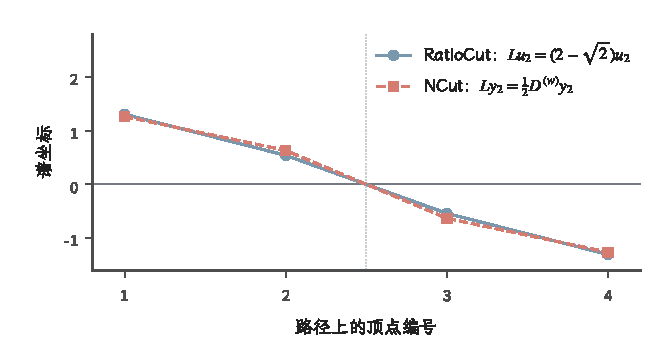
\includegraphics[width=\linewidth]{figures/01-mathematical-preliminaries/03-graphs-and-signals/matplotlib/teaching-graph/spectral-coordinates.pdf}
  \caption{单位权四顶点路径的两种谱方向。蓝实线为组合拉普拉斯第二特征向量，
  红虚线为度加权广义特征向量，点形也作区分。显示时均按欧氏范数\(2\)缩放，
  不替代NCut的度加权范数。横轴为四个离散顶点，连线仅引导阅读；
  竖虚线标出零阈值分割，两种方向虽同号分组，相对幅度并不相同。}
  \label{fig:graph-theory-spectral-coordinates}
\end{figure}

取整以后必须回到原离散目标核验质量。特征向量的方向稳定性还依赖相邻特征值间隔：
与其他特征值的间隔很小时，小扰动可能使方向明显旋转；
重特征值时应考察对应子空间，只有它与其余谱充分分离时才能谈相应稳定性，
不能把任意单个基向量当成固有划分。

\subsection{离散选择的近似与质量验证}

前面的谱划分已经展示了通用做法：扩大可行域获得下界，
再恢复原约束下的方案获得上界。仅把\(z_i\in\{0,1\}\)改成\(z_i\in[0,1]\)
还没有完整指定松弛，必须说明连续域上的目标怎样定义。
记原可行集为\(\mathcal Z\)，选
\(\widetilde{\mathcal Z}\supseteq\mathcal Z\)及延拓\(\widetilde{\mathcal E}\)，要求
\[
  \widetilde{\mathcal E}(\bm z)=\mathcal E(\bm z)\quad(\bm z\in\mathcal Z).
\]
则
\[
  L_{\mathrm{relax}}
  =\inf_{\bm z\in\widetilde{\mathcal Z}}\widetilde{\mathcal E}(\bm z)
  \leq \mathcal E^\star
  =\min_{\bm z\in\mathcal Z}\mathcal E(\bm z).
\]
不同延拓即使在离散点上一致，也可能得到不同下界。
若松弛最优值达到，且存在一个松弛最优解属于原可行集，它同时就是离散全局最优解；
分数解则还需要取整、局部搜索或分支定界。

恢复出可行配置\(\widehat{\bm z}\)以后，令\(U=\mathcal E(\widehat{\bm z})\)，
任何有效下界\(L\leq\mathcal E^\star\)都给出
\[
  0\leq U-\mathcal E^\star\leq U-L.
\]
\(U-L\)是次优差距的上界，不是实际误差；仅在下界紧时二者相等。
数值求解器当前的连续可行目标通常是松弛最优值的上界，
不能未经对偶证书或误差控制就把它称为原问题下界。
逐坐标按\(1/2\)阈值取整也可能破坏总数、连通等全局约束；
必须先检查恢复方案可行，才有上界\(U\)。

确定性取整需要逐实例的质量证明。采用随机取整时，还须利用后续
第~\ref{chap:random-variables}章的概率工具说明抽样规则、平均误差与修复可行性的代价；
本节的上下界证书则逐个检查所得到的方案。非负且\(\mathcal E^\star>0\)时，
\(U\leq\alpha\mathcal E^\star\)表达乘法近似比；目标可能为负或最优值为零时，
加法误差\(U-\mathcal E^\star\leq\varepsilon\)更适合。
运行快、连续目标下降与离散方案已最优是不同结论。

\section{图上的函数与传播}
\label{sec:graph-theory-functions-propagation}

图上“每点一个数”与“每种配置一个数”有不同定义域。
前者是\(f:V\to\mathbb R\)，四顶点图只需四个值；
后者是\(F:\mathcal Z_1\times\cdots\times\mathcal Z_4\to\mathcal S\)，
四个二值变量已有\(16\)种配置。
对前者汇总邻居，会改变一个顶点信号；对后者汇总变量，会产生边缘表或最优值。
二者都能沿图局部计算，却不能据此互换含义。

\subsection{顶点函数的变换与传播}
\label{sec:graph-theory-vertex-functions}
\label{sec:graph-theory-structure-comparison}

顶点数值可以表达温度、得分或某个观测通道；顶点标记则可以表达类别或局部结构类型。
数值允许线性叠加，离散标记未必有加法，因此分别使用谱变换和邻域细化。
重编号只是坐标改变，两种运算都需要检查是否随顶点同步重排。

\subsubsection{数值信号的谱变换与局部传播}
\label{sec:signal-analysis-graph-state-kernels}

一个\term{图信号}（graph signal）是给每个顶点一个数的函数，
固定编号后写成\(\bm f\in\mathbb R^n\)。
规则序列可以统一向前平移一步，一般图却没有唯一的全局“下一个顶点”。
这里回用第~\ref{sec:graph-theory-vertex-configuration}节的组合拉普拉斯，
用沿边变化的能量确定适合本图的坐标，而不预设规则时间轴上的傅里叶公式。

谱定理给出
\[
  \bm L=\bm U\bm\Lambda\bm U^\top,\qquad
  \bm U^\top\bm U=\bm I,\qquad
  \bm\Lambda=\operatorname{diag}(\lambda_1,\ldots,\lambda_n).
\]
其中\(0=\lambda_1\leq\cdots\leq\lambda_n\)。
\begin{definition}[图傅里叶变换]
  \label{def:signal-analysis-graph-fourier-transform}
  选定\(\bm L\)的一组实标准正交特征向量作为\(\bm U\)的列，
  图信号的\term{图傅里叶变换}（graph Fourier transform）及逆变换为
  \begin{equation}
    \widehat{\bm f}_{\mathcal G}=\bm U^\top\bm f,\qquad
    \bm f=\bm U\widehat{\bm f}_{\mathcal G}.
    \label{eq:signal-analysis-graph-fourier}
  \end{equation}
\end{definition}

正交性使变换不丢信息，并有
\[
  \|\bm f\|_2^2=\sum_{k=1}^n|\widehat f_{\mathcal G,k}|^2,\qquad
  \bm f^\top\bm L\bm f
  =\sum_{k=1}^n\lambda_k|\widehat f_{\mathcal G,k}|^2.
\]
所以小特征值的单位模态沿边变化较小，大特征值的单位模态变化较大，
这就是把\(\lambda_k\)称为图频率尺度的根据。
若有重特征值，对应空间内可旋转正交基，单个坐标随之改变，
该子空间上的投影及系数平方和却不变。图频率先对应特征空间，
不总是一个唯一的特征向量；即使简单特征值的实特征向量也有正负号自由度。

单位权简单环提供与规则序列相接的例子。取\(N\geq3\)，
顶点局部编号\(r=0,\ldots,N-1\)，每点连到模\(N\)的左右邻居。
这里的模态指标\(k=0,\ldots,N-1\)按复指数编号，不按前面的特征值大小排序。
直接计算
\[
  (\bm L\bm f)[r]=2f[r]-f[(r-1)\bmod N]-f[(r+1)\bmod N].
\]
令\(u_k[r]=N^{-1/2}e^{2\pi\mathrm i kr/N}\)，则
\begin{align*}
  (\bm L\bm u_k)[r]
  &=\left(2-e^{-2\pi\mathrm i k/N}-e^{2\pi\mathrm i k/N}\right)u_k[r]\\
  &=\left(2-2\cos\frac{2\pi k}{N}\right)u_k[r].
\end{align*}
不同\(k\)的内积为有限几何和：
\(\frac1N\sum_{r=0}^{N-1}e^{2\pi\mathrm i(k-\ell)r/N}\)
在\(k=\ell\)时为\(1\)，否则为\(0\)。
故这些模式组成复酉基，坐标变换用\(\bm U^*\bm f\)，逆变换用\(\bm U\)，
不能把实情形的转置直接用于复基。这些复指数模式与前章
定义~\ref{def:signal-analysis-dft}中的DFT使用同一组振荡函数；这里以
\(N^{-1/2}\)归一化基向量，所以图谱系数等于相应DFT系数除以\(\sqrt N\)。
直接代入环图算子并检查正交性，说明同一组模式为何既适合循环平移，也适合环图能量。
\(N=2\)时简单图的左右邻居重合，不能继续把该单边图写成度为\(2\)的上述环算子。

环图的\(k\)和\(N-k\)具有相同特征值，因而图能量并不区分两种复振荡方向。
一般图的模式还依赖连接、边权和归一化选择；
两个不同图上的第\(k\)个系数没有天然相同的物理频率。
跨图比较须依赖共同图构造、谱区间或子空间语义，不能仅按坐标序号对齐。

谱坐标建立以后，可以按标量响应\(g\)放大或缩小不同模态：
\[
  g(\bm L)=\bm U g(\bm\Lambda)\bm U^\top,\qquad
  \bm y=g(\bm L)\bm f,\qquad
  \widehat y_{\mathcal G,k}=g(\lambda_k)\widehat f_{\mathcal G,k}.
\]
相同特征值必须使用相同标量响应，所以\(g(\bm L)\)不依赖重特征空间内的任意基选择。
若对同一特征值的不同基向量随意赋不同系数，得到的就不是这个标量矩阵函数。

若响应是\(K\)次多项式，
\begin{equation}
  g(\bm L)=\sum_{r=0}^K\alpha_r\bm L^r,
  \label{eq:graph-theory-polynomial-filter}
\end{equation}
则滤波写成
\begin{equation}
  \bm y=\sum_{r=0}^K\alpha_r\bm L^r\bm f.
  \label{eq:signal-analysis-polynomial-graph-filter}
\end{equation}
一次乘\(\bm L\)只使用本点和一跳邻居的值。
归纳地，若\((\bm L^r)_{i,j}\neq0\)，矩阵乘积中必须存在至多\(r\)步的支撑图行走
从\(i\)到\(j\)，对角因子允许停留；因此图距离大于\(K\)时滤波矩阵条目为零。
“至多\(K\)跳”是依赖范围上界，不保证范围内每点的系数非零，
因为权重和多项式系数可能相消。
给定稀疏图及多项式系数，反复乘矩阵即可计算，无需显式对角化；
每步成本为\(O(|V|+|E_+|)\)。

三顶点路径的例子同时检验数值和范围：
\[
  \bm L=
  \begin{bmatrix}1&-1&0\\-1&2&-1\\0&-1&1\end{bmatrix},\qquad
  \bm f=(1,0,0)^\top,\qquad g(\lambda)=1-\lambda/3.
\]
于是
\[
  \bm H\bm f=(\bm I-\bm L/3)\bm f=(2/3,1/3,0)^\top.
\]
首点的数值只到一跳邻居。该图特征值为\(0,1,3\)，响应为\(1,2/3,0\)，
所以同一操作在谱坐标中消除了最高频模式。
再作用一次，
\[
  \bm H^2\bm f
  =(\bm I-2\bm L/3+\bm L^2/9)\bm f=(5/9,1/3,1/9)^\top,
\]
第三点才收到非零值，符合二次多项式的两跳范围。

\begin{figure}[htbp]
  \centering
  \begingroup
\begin{tikzpicture}[x=1mm,y=1mm,text=FigureInk,
  font=\figurefont\footnotesize,
  vertex/.style={circle,draw=FigureStroke,fill=white,line width=.9pt,
    minimum size=7mm,inner sep=0pt},
  existing/.style={vertex,fill=FigureBlueFill},
  reached/.style={vertex,fill=FigureRedFill},
  edge/.style={draw=FigureStroke,line width=1pt},
  note/.style={inner sep=0pt,fill=none}
]
  \path[use as bounding box] (0,0) rectangle (112,72);
  \foreach \y/\operator in {60/{\bm f},37/{\bm H\bm f},14/{\bm H^2\bm f}} {
    \node[note,anchor=east] at (24,\y) {\(\operator\)};
  }
  \node[existing] (a0) at (42,60) {\(1\)};
  \node[vertex] (b0) at (68,60) {\(2\)};
  \node[vertex] (c0) at (94,60) {\(3\)};
  \node[existing] (a1) at (42,37) {\(1\)};
  \node[reached] (b1) at (68,37) {\(2\)};
  \node[vertex] (c1) at (94,37) {\(3\)};
  \node[existing] (a2) at (42,14) {\(1\)};
  \node[existing] (b2) at (68,14) {\(2\)};
  \node[reached] (c2) at (94,14) {\(3\)};
  \foreach \r in {0,1,2} {
    \draw[edge] (a\r) -- (b\r) -- (c\r);
  }
  \foreach \x/\y/\value in {
    42/52/1,68/52/0,94/52/0,
    42/29/{2/3},68/29/{1/3},94/29/0,
    42/6/{5/9},68/6/{1/3},94/6/{1/9}} {
    \node[note] at (\x,\y) {\(\value\)};
  }
\end{tikzpicture}
\endgroup

  \caption{三顶点路径上的一次与二次局部滤波。顶点下方为精确值，
  白色表示零值，浅蓝表示此前已非零的顶点，浅红表示本步新到达的顶点；
  初始非零点也用浅蓝标出。颜色不编码连续色标。
  图的边均为单位权无向边，没有时间箭头；从上行到下行表示反复作用
  \(\bm H=\bm I-\bm L/3\)。两步结果的算子是二次多项式，能到达两跳邻居。}
  \label{fig:graph-theory-polynomial-locality}
\end{figure}
\FloatBarrier

这种谱滤波有时也称图卷积，但一般没有规则网格上那种唯一的核平移。
改变图或改用归一化拉普拉斯，同一个\(g\)会产生不同空间作用。
局部多项式只是本图算子的函数，不自动继承普通平移卷积的全部性质。

还要检查编号是否影响结果。顶点级输出应随重编号同步重排，称为等变；
整图级输出应保持相同，称为不变，完整定义见
定义~\ref{def:geometry-equivariant-map}和定义~\ref{def:geometry-invariant-map}。
对第~\ref{sec:graph-theory-graph-isomorphism}节的置换矩阵\(\bm P\)，
\begin{equation}
  \begin{aligned}
    \bm W'&=\bm P\bm W\bm P^\top,\qquad
    \bm D^{(w)\prime}=\bm P\bm D^{(w)}\bm P^\top,\\
    \bm L'&=\bm P\bm L\bm P^\top.
  \end{aligned}
  \label{eq:graph-theory-laplacian-relabel}
\end{equation}
若\(\bm f'=\bm P\bm f\)，则\(\bm L'\bm f'=\bm P\bm L\bm f\)。
更一般地，由\(\bm P^\top\bm P=\bm I\)相邻消去，
\[
  g(\bm L')\bm f'
  =\sum_{r=0}^K\alpha_r(\bm P\bm L\bm P^\top)^r\bm P\bm f
  =\bm P g(\bm L)\bm f.
\]
故多项式滤波等变；后接对顶点求和等对称读出，就得到不变的图级表示。
不变性只排除任意编号的影响，不保证不同非同构图一定得到不同结果。

有限次滤波每次最多增加有限跳数；连续时间扩散则把局部差分累计成矩阵指数。
若每点按邻居与自身的差调整，
\(f_i'(t)=\sum_jw_{i,j}(f_j(t)-f_i(t))\)，就得到
\begin{equation}
  \frac{\mathrm d\bm f(t)}{\mathrm dt}=-\bm L\bm f(t),\qquad
  \bm f(0)=\bm f_0.
  \label{eq:graph-theory-heat-equation}
\end{equation}
第~\ref{chap:matrix-analysis}章的矩阵指数给出
\[
  \bm f(t)=e^{-t\bm L}\bm f_0
  =\sum_{k=1}^ne^{-t\lambda_k}
    \langle\bm u_k,\bm f_0\rangle\bm u_k.
\]
各坐标独立按\(e^{-t\lambda_k}\)衰减，零模保持，大特征值模式衰减更快。
对任一支撑连通分量\(C\)，常量单位向量为\(\bm1_C/\sqrt{|C|}\)，
其投影在每点的值为\(|C|^{-1}\sum_{i\in C}f_{0,i}\)。
其余正特征值项趋于零，所以每个分量分别趋于自己的初始平均；
支撑连通时才是全图同一平均。

守恒和耗散也可不经对角化验证。由\(\bm1^\top\bm L=\bm0^\top\)，
\[
  \frac{\mathrm d}{\mathrm dt}\bm1^\top\bm f(t)
  =-\bm1^\top\bm L\bm f(t)=0.
\]
平方范数与Dirichlet能量不能混称为同一个能量：
\[
  \frac{\mathrm d}{\mathrm dt}\frac12\|\bm f(t)\|_2^2
  =\bm f(t)^\top\bm f'(t)
  =-\bm f(t)^\top\bm L\bm f(t)\leq0.
\]
边差能量的导数则为
\begin{align*}
  \frac{\mathrm d}{\mathrm dt}\bigl[\bm f(t)^\top\bm L\bm f(t)\bigr]
  &=\bm f'(t)^\top\bm L\bm f(t)+\bm f(t)^\top\bm L\bm f'(t)\\
  &=-2\bm f(t)^\top\bm L^2\bm f(t)
   =-2\|\bm L\bm f(t)\|_2^2\leq0.
\end{align*}
对称性保证两项相同。平方范数下降率等于负边差能量，
边差能量本身的下降率又多一个拉普拉斯，两个结论各有不同内容。

贯穿图取单位边权、\(\bm f_0=(1,0,0,0)^\top\)，其谱为\(0,2,4,4\)。
不同模态的保留比例为\(1,e^{-2t},e^{-4t}\)，重特征值\(4\)的两个方向同速衰减。
图连通且总和为\(1\)，所以极限为每点\(1/4\)，不是全部数值归零。

\begin{figure*}[htbp]
  \centering
  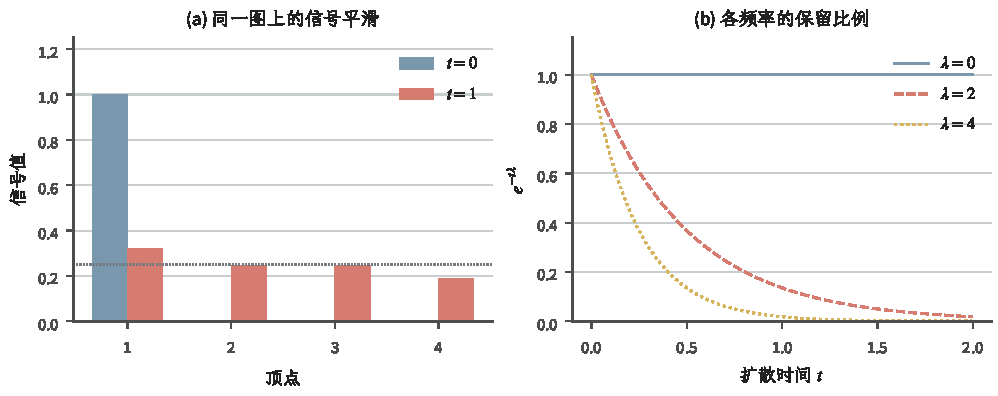
\includegraphics[width=\linewidth]{figures/01-mathematical-preliminaries/03-graphs-and-signals/matplotlib/probability-discrete/graph-diffusion-spectrum.pdf}
  \caption{贯穿四顶点图的解析式扩散。左图比较\(\bm f(0)=(1,0,0,0)^\top\)
  与\(\bm f(1)=e^{-\bm L}\bm f(0)\)，灰虚线是最终均值\(1/4\)；
  右图绘制特征值\(0,2,4\)的保留比例，\(4\)的重数为\(2\)。
  柱和曲线直接由该图的拉普拉斯计算，不表示实验均值或误差条。}
  \label{fig:graph-diffusion-spectrum}
\end{figure*}

指数一般不是固定低阶多项式，因此不能把有限次滤波的固定跳数截断套到它上面。
扩散使总边差能量不增，却不保证每条边两端的差都单调缩小。
例如单位权路径\(1-2-3\)从\(\bm f(0)=(1,1,0)^\top\)出发时，
\(\bm f'(0)=-\bm L\bm f(0)=(0,-1,1)^\top\)。
边\(1-2\)的初始差为零，差的导数却为\(1\)，因此短时间内两端会从相等变为不等；
此时总边差能量的导数仍为\(-4\)。整体耗散与逐边单调是两个不同的要求。
扩散也不保证保留预测所需的类别边界，时间过长会抹去同一支撑分量内的全部非恒定差异。

图Dirichlet能量还与第~\ref{chap:differential-geometry-and-symmetry}章的连续能量
\[
  \int_{\mathcal M}\|\operatorname{grad}f\|_g^2\,\mathrm dV_g
\]
形成离散与连续的对应：前者比较采样点之间的有限差分，
后者累计无穷小方向的变化。但形式相似不构成收敛定理。
若图来自点云，采样密度、邻域半径或核带宽、权重缩放、归一化及边界条件
共同决定可能的极限。邻域太大可能连接流形不同折，太小则可能断连；
未校正的不均匀采样可能导出带密度漂移的算子，
而不是仅由Riemann体积确定的Laplace--Beltrami算子。
离散谱结论相对于已选图精确成立，连续近似和任务语义仍各需额外条件。

\subsubsection{离散标记的邻域细化}

数值滤波考察信号变化，结构比较则常需知道各点周围有哪些类型的邻居。
只记录出现过哪些类型会丢掉次数；按编号排列又依赖任意顺序。
\term{多重集合}（multiset）保留种类与次数、忽略排列：
\(\{\!\{a,a,b\}\!\}\)与\(\{\!\{a,b\}\!\}\)不同。

\begin{definition}[一维邻域标记细化]
  \label{def:graph-theory-wl-refinement}
  一维Weisfeiler--Leman细化（1-dimensional Weisfeiler--Leman refinement, 1-WL）
  从初始标记\(c_i^{(0)}\)出发，同步更新
  \begin{equation}
    c_i^{(t+1)}=\operatorname{HASH}\left(
      c_i^{(t)},\left\{\!\left\{c_j^{(t)}:j\in N(i)\right\}\!\right\}
    \right),
    \label{eq:graph-theory-wl-refinement}
  \end{equation}
  其中\(\operatorname{HASH}\)对不同输入对给出不同新标记。
\end{definition}

这里是无碰撞编码的数学约定，不是普通有限哈希函数永不碰撞的承诺。
比较两图时必须共享初始标记规则和编码对应，
例如在两图的不交并上统一编码，不能各自随意命名后比较字面值。
同构只重排顶点及其邻居，所以每轮标记同步重排，各标记出现次数不变。
上述版本仅用无向邻域；有向或带边属性的细化需要相应扩充输入，不能无声丢掉方向和属性。

令\(\mathcal P^{(t)}\)为相同标记构成的分区。
更新包含自身旧标记，所以旧标记不同的两点下一轮仍不同；
\(\mathcal P^{(t+1)}\)只能细分，不能合并。
每次严格细分至少增加一个非空块，而\(n\)点最多有\(n\)块，
因此严格细分至多\(n-1\)次。
若某轮分区未变，同一块中的顶点已有相同的各旧块邻居计数，
给这些块统一换新标记不会改变计数相等性，下一轮也不能再拆分，
归纳可知以后一直稳定。稳定指等价类不再细分，符号名称仍可换新。

稳定不等于已判定同构。所有顶点初始同标记时，六环\(C_6\)与两个不相连三角形
都让每点看到两个同标记邻居，归纳地每轮仍同标记，两图各有六个此类顶点。
1-WL无法区分它们，尽管前者连通、后者不连通。

\begin{figure}[htbp]
  \centering
  \begingroup
% Local styles; callers keep this input inside a group.
\tikzset{
  reader vertex/.style={circle,draw=FigureStroke,fill=white,line width=1pt,
    minimum size=7mm,inner sep=0pt,font=\figurefont\footnotesize,text=FigureInk},
  reader factor/.style={rectangle,draw=FigureStroke,fill=FigureYellowFill,
    line width=1pt,minimum size=8mm,inner sep=2pt,font=\figurefont\footnotesize},
  reader edge/.style={draw=FigureStroke,line width=1.1pt},
  reader arrow/.style={reader edge,-{Stealth[length=2.2mm,width=1.4mm]}},
  reader label/.style={font=\figurefont\footnotesize,text=FigureInk},
  reader note/.style={reader label,fill=white,inner sep=1pt},
  reader highlight/.style={draw=FigureYellow,line width=1.1pt},
  reader auxiliary/.style={draw=FigureMuted,line width=0.6pt,dashed}
}

\begin{tikzpicture}[text=FigureInk]
  \node[reader label] at (0,1.7) {(a) 六顶点环 \(C_6\)};
  \foreach \i in {1,...,6}
    \node[reader vertex,fill=FigureYellowFill] (a\i) at ({90-60*(\i-1)}:1.1) {};
  \foreach \i/\j in {1/2,2/3,3/4,4/5,5/6,6/1}
    \draw[reader edge] (a\i)--(a\j);
  \node[reader label] at (5.2,1.7) {(b) 两个不相交三角形};
  \foreach \x/\prefix in {3.8/b,6.6/c}
  {
    \node[reader vertex,fill=FigureYellowFill] (\prefix1) at (\x,0.9) {};
    \node[reader vertex,fill=FigureYellowFill] (\prefix2) at (\x-0.75,-0.6) {};
    \node[reader vertex,fill=FigureYellowFill] (\prefix3) at (\x+0.75,-0.6) {};
    \draw[reader edge] (\prefix1)--(\prefix2)--(\prefix3)--(\prefix1);
  }
  \node[reader label] at (0,-1.85) {每个顶点：2个同标记邻居};
  \node[reader label] at (5.2,-1.85) {每个顶点：2个同标记邻居};
\end{tikzpicture}
\endgroup

  \caption{同样的邻居标记计数可以来自不同全局结构。两张六顶点图初始同标记，
  每轮每点仍见到两个同标记邻居，故1-WL计数无法区分一条六环与两个三角形。
  这不表示连通性难计算，而是说明该细化遗漏了这一差异。
  浅黄只表示共同标记，不加入唯一编号，以保持无标记图的比较设定。}
  \label{fig:graph-theory-wl-local-ambiguity}
\end{figure}

给每个顶点附任意唯一编号不是无条件补救：若重编号后重新按编号赋特征，
输出会依赖命名；若把额外属性随置换同步移动，可以保持等变，
但问题已变成带属性图的比较。
具体图网络的共享更新、聚合和读出能否达到或超过某种细化的区分能力，
还须在模型章节依据函数族证明。结构等变性不等于完全可辨，更不等于泛化保证。

\subsection{配置函数的汇总与查询}
\label{sec:graph-theory-semiring-dynamic-programming}

现在每个顶点\(i\)代表变量\(z_i\)，取值于非空有限集合\(\mathcal Z_i\)；
贯穿例取\(\mathcal Z_i=\{0,1\}\)。
配置函数\(F(\bm z)\)评价全部变量的一次完整赋值。
图记录哪些变量同时进入局部函数，查询则另行规定要输出总权重、最优值，
还是保留部分变量的函数表。只有明确输出以后，“消去变量”才有确定含义。

\subsubsection{配置查询的目标与半环运算}

先不谈分解，直接看两变量表
\[
  g(x,y)=
  \begin{array}{c|cc}
    &y=0&y=1\\ \hline
    x=0&1&3\\
    x=1&2&4
  \end{array}.
\]
若数字是非负权重，总权重与最佳权重分别为
\[
  \sum_{x,y}g(x,y)=10,\qquad \max_{x,y}g(x,y)=4.
\]
最佳权重的见证为\((1,1)\)。
若同一数字解释为成本，最低成本为\(1\)，见证变为\((0,0)\)。
关系图相同，甚至表也相同，仍不能替读者决定查询。

若输出要保留\(y\)，求和消去\(x\)得到
\(m(y)=\sum_xg(x,y)\)，即\(m(0)=3,m(1)=7\)。
这是一张表，再汇总\(y\)才得标量\(10\)。
将每格权重除以\(10\)，得到给各对\((x,y)\)分配份额的联合概率表；
各格非负，全部份额相加为\(1\)。把具有同一\(y\)的份额相加，得到只记录\(y\)
的边缘概率，所以这里\(y=0,1\)的概率分别是\(3/10,7/10\)。
这一步只需对有限表求和；一般概率分布将在第~\ref{chap:random-variables}章定义。
若改为最大化，得到\(m(0)=2,m(1)=4\)，记录每个\(y\)的最佳权重，
不再是边缘概率。消元是汇总内部变量的贡献，不是删除它的约束。

为某个固定配置组合局部项，与跨不同配置汇总结果，是两种操作。
普通权重用乘法组合、加法汇总；成本用加法组合、最小值汇总。
分别记为\(\otimes\)和\(\oplus\)，核心规则是：不依赖被汇总变量的项可移到汇总外。

\begin{definition}[交换半环]
  \label{def:graph-theory-semiring}
  本章使用的交换\term{半环}（semiring）记为
  \[
    (\mathcal S,\oplus,\otimes,e_{\oplus},e_{\otimes}),
  \]
  包含一个集合、两种运算及其单位元。
  两种运算分别结合且交换，单位元分别为\(e_{\oplus}\)、\(e_{\otimes}\)，并满足
  \[
    a\otimes(b\oplus c)=(a\otimes b)\oplus(a\otimes c),\qquad
    a\otimes e_{\oplus}=e_{\oplus}.
  \]
  空汇总取\(e_{\oplus}\)，空组合取\(e_{\otimes}\)。
\end{definition}

半环不要求加法逆元或乘法逆元；这里的局部算法不需减法和除法。
几个具体实例为
\[
  \begin{array}{c|c|c|c|c}
    \text{用途}&\mathcal S&\oplus&\otimes&(e_{\oplus},e_{\otimes})\\ \hline
    \text{总权重}&\mathbb R_{\geq0}&+&\times&(0,1)\\
    \text{最大权重}&\mathbb R_{\geq0}&\max&\times&(0,1)\\
    \text{最小成本}&\mathbb R\cup\{+\infty\}&\min&+&(+\infty,0)\\
    \text{是否可行}&\{\mathrm{false},\mathrm{true}\}&\lor&\land&
       (\mathrm{false},\mathrm{true})
  \end{array}
\]
最大积中的\(0\)既是最大值运算的单位元，也是乘法吸收元。
最小加法约定\(+\infty+c=+\infty\)，用正无穷表达不可行。
对数域还可用\((\mathbb R\cup\{-\infty\},\max,+,-\infty,0)\)，
约定\(-\infty+c=-\infty\)。这些选择改变答案，不能只当成实现细节。

再引入局部因子。贯穿图上的一元与成对专门情形为
\begin{equation}
  F(\bm z)=\bigotimes_{i\in V}\phi_i(z_i)
    \otimes\bigotimes_{\{i,j\}\in E}\phi_{i,j}(z_i,z_j).
  \label{eq:graph-theory-factorized-objective}
\end{equation}
因子是局部函数，作用域是它依赖的变量集合。
若要表达原三元子句，仍须保留\(\phi_{2,3,4}(z_2,z_3,z_4)\)；
上述成对公式不是从三个两两关系恢复三元约束的等价式。
一般可写\(F(\bm z)=\bigotimes_a\phi_a(\bm z_{S_a})\)，
其中\(S_a\subseteq V\)为任意有限作用域。
改变作用域会改变分解和计算成本，即使某些数值条目恰好相同。

例如和积下要保留\(z_4\)，查询为
\[
  Q(z_4)=\sum_{z_1,z_2,z_3}F(\bm z),\qquad
  Z=\sum_{z_4}Q(z_4).
\]
只有在\(F\)是非负权重且\(0<Z<\infty\)时，\(F/Z\)才为每个完整配置分配
非负且总和为\(1\)的概率，\(Q(z_4)/Z\)才是只保留\(z_4\)的边缘概率。
若总权重为零，就不能作这种归一化。若改问最低成本，目标为
\(\min_{\bm z}[\sum_i c_i(z_i)+\sum_{\{i,j\}\in E}c_{i,j}(z_i,z_j)]\)，
就须同时更换组合和汇总。图本身不自动添加概率、因果或时间语义。

\subsubsection{基于变量消元的查询与恢复}

第~\ref{sec:graph-theory-elimination-width}节已说明消元如何改变作用域，
现在证明它如何保持数值查询。
每次收集全部含\(z_i\)的当前因子\(\mathcal F_i\)，合并其作用域并去掉\(i\)，
记剩余接口为\(R_i\)，生成
\[
  \psi_i(\bm z_{R_i})
  =\bigoplus_{z_i\in\mathcal Z_i}\ \bigotimes_{f\in\mathcal F_i}f.
\]
删去这些旧因子，以\(\psi_i\)替换；其余因子保持不动。
这不是丢掉\(z_i\)的影响，而是对每个剩余接口值预先算出它的全部贡献。
完整消元的目标，在贯穿成对例中为
\begin{equation}
  Z=\bigoplus_{\bm z\in\mathcal Z_1\times\cdots\times\mathcal Z_4}
  \left[
    \bigotimes_i\phi_i(z_i)
    \otimes\bigotimes_{\{i,j\}\in E}\phi_{i,j}(z_i,z_j)
  \right].
  \label{eq:graph-theory-semiring-elimination}
\end{equation}

\begin{theorem}[半环变量消除的正确性]
  \label{thm:graph-theory-semiring-elimination}
  对有限取值变量和交换半环，按任意完整次序对有限个局部因子执行上述消元，
  所得标量等于直接枚举的全局汇总。
  特别地，式~\eqref{eq:graph-theory-factorized-objective}得到
  式~\eqref{eq:graph-theory-semiring-elimination}。
  若保留一组输出变量，在其余变量消去后停止，所得表逐个输出配置等于原查询。
\end{theorem}

\begin{proof}
维持更强的不变量：对每个尚未消去变量的固定配置，
当前因子的半环组合等于原函数对已消去变量的汇总。
初始没有已消变量，不变量即为原局部分解。

设下一变量是\(z_i\)，把当前因子分成含它的\(\mathcal F_i\)和不含它的
\(\mathcal F_{-i}\)。固定其他变量，有限性和分配律给出
\[
  \bigoplus_{z_i}
  \left[
    \left(\bigotimes_{f\in\mathcal F_{-i}}f\right)
    \otimes\left(\bigotimes_{f\in\mathcal F_i}f\right)
  \right]
  =
  \left(\bigotimes_{f\in\mathcal F_{-i}}f\right)
  \otimes\left(\bigoplus_{z_i}\bigotimes_{f\in\mathcal F_i}f\right).
\]
右侧最后一项就是新因子\(\psi_i\)。结合律与交换律允许把对\(z_i\)的汇总
接在此前已消变量的有限汇总之后，因而新的当前组合等于原函数对全部已消变量的汇总，
不变量保持。
若再对剩余变量汇总，上式也表明每一步的全局值不变：
\begin{align*}
  &\bigoplus_{\bm z_{-i}}\bigoplus_{z_i}
    \left[\left(\bigotimes_{f\in\mathcal F_{-i}}f\right)
       \otimes\left(\bigotimes_{f\in\mathcal F_i}f\right)\right]\\
  &\qquad=\bigoplus_{\bm z_{-i}}
    \left[\left(\bigotimes_{f\in\mathcal F_{-i}}f\right)\otimes\psi_i\right].
\end{align*}
归纳到所有变量消去，只剩直接枚举的标量。
若输出变量不消去，同一逐配置不变量即给出所需函数表。
\end{proof}

正确性允许任意次序，中间表成本却不相同。
贯穿图先消去\(1,4\)只需保留接口\(\{2,3\}\)；
先消去\(2\)则形成对\(\{1,3,4\}\)的表，并出现填充边\(\{1,4\}\)。
结构部分给出的\(q^{k+1}\)工作表界因此控制实际消元，而不改变查询定义。

和积得到的是未归一化权重；保留输出变量后仍需除以同一总权重，
并检查总权重严格为正。最大积则得到
\[
  M=\max_{\bm z}\prod_i\phi_i(z_i)
        \prod_{\{i,j\}\in E}\phi_{i,j}(z_i,z_j).
\]
只存最大值不能恢复最优配置。
每次对接口配置保存一个达到最大值的\(z_i\)，最后从末次选择开始，
按消元逆序用已知接口值查回选择，即能恢复一个全局见证。
每一步都保存条件最优选择，反向代入使该步达到原先记录的局部最优值，
归纳便得到全局值\(M\)。并列时须声明固定平局规则、返回任意一个或枚举全部；
枚举全部的输出规模可能很大。

最小加法同理求得
\[
  C^\star=\min_{\bm z}
    \left[\sum_i c_i(z_i)+\sum_{\{i,j\}\in E}c_{i,j}(z_i,z_j)\right],
\]
并保存条件最小选择回溯；若最优值为\(+\infty\)，就应报告没有有限成本可行配置。
严格正权重可用负对数把最大积转成最小加法，
因为乘积变为和，负对数反转大小次序。
零权重约定映为\(+\infty\)，负权重则没有直接的实对数解释；
若用普通对数，得到的是最大加法而非最小加法。

同一种有限汇总可换序，不同汇总通常不行。
取
\[
  h(x,y)=
  \begin{array}{c|cc}
    &y=0&y=1\\ \hline
    x=0&4&0\\
    x=1&0&4
  \end{array}.
\]
要求先固定同一个\(x\)、再累计全部\(y\)，得到
\begin{equation}
  \max_x\sum_yh(x,y)=4.
  \label{eq:graph-theory-max-sum-order-a}
\end{equation}
允许每个\(y\)分别选择最佳\(x\)，则为
\begin{equation}
  \sum_y\max_xh(x,y)=8.
  \label{eq:graph-theory-max-sum-order-b}
\end{equation}
区别是是否允许选择随\(y\)而改变。
一般对有限实值表，
\[
  \max_x\sum_yh(x,y)\leq\sum_y\max_xh(x,y),
\]
因为对任意固定\(x\)，每个\(h(x,y)\leq\max_{x'}h(x',y)\)，
相加再最大化仍保序。
若某个共同\(x\)在所有\(y\)上同时最大，显然取等号；
反过来，若取等号，取左侧一个最优\(x\)，逐项非负差的总和为零，
故每项都为零，也就必须有这样一个共同最优选择。

混合求和与最大化因此限制合法消元次序，最小可用宽度可能超过普通树宽。
按配置份额求和得到边缘概率、直接寻找权重最大的完整配置，以及先求和再对保留变量
最大化，是不同的查询，不能混用目标或消元次序。
把有限和改成连续积分，还须回用定理~\ref{thm:analysis-tonelli-fubini}：
在\(\sigma\)有限乘积测度下，非负可测函数可由Tonelli换序，
带符号函数通常需要Fubini的绝对可积条件。
把求和号改成积分号不自动保证存在性、换序或有限表算法仍适用。

\subsubsection{基于树形消息的局部查询}

消元把内部变量压缩成接口表；树消息则按固定的树形接口复用这些表。
在贯穿图的一元与成对情形中，先消去\(z_1\)所得表为
\begin{equation}
  m_{1\to\{2,3\}}(z_2,z_3)=
  \bigoplus_{z_1\in\mathcal Z_1}
  \phi_1(z_1)\otimes\phi_{1,2}(z_1,z_2)\otimes\phi_{1,3}(z_1,z_3).
  \label{eq:graph-theory-interface-message}
\end{equation}
同样计算\(z_4\)一侧的\(m_{4\to\{2,3\}}\)，
再在接口上组合两条消息与\(\phi_2,\phi_3,\phi_{2,3}\)，最后汇总\(z_2,z_3\)。
若还有三元因子\(\phi_{2,3,4}\)，应把它完整纳入\(4\)侧表。
每种接口配置的局部结果只算一次。

合法性的直接原因是分配律，而不只是图形看起来分成两侧。
对不依赖\(z_1\)的项\(c(z_2,z_3)\)，
\[
  \bigoplus_{z_1}\bigl(c(z_2,z_3)\otimes g(z_1,z_2,z_3)\bigr)
  =c(z_2,z_3)\otimes\bigoplus_{z_1}g(z_1,z_2,z_3).
\]
图确定哪些项与内部变量无关，半环公理允许移出汇总，
接口表则保存可复用的子问题答案。

先在一棵树上严格定义消息。顶点放一元因子，边放成对因子；
删去\(\{u,v\}\)，记\(u\)侧连通分量为\(T_{u\mid v}\)。
消息不是只汇总顶点\(u\)，而是汇总整棵\(u\)侧子树：
\begin{equation}
  \begin{aligned}
    m_{u\to v}(z_v)
    =\bigoplus_{\bm z_{T_{u\mid v}}}
    \biggl[
      &\bigotimes_{i\in T_{u\mid v}}\phi_i(z_i)\\[-2pt]
      {}\otimes&
      \bigotimes_{\substack{\{i,j\}\in E\\i,j\in T_{u\mid v}}}
        \phi_{i,j}(z_i,z_j)
      \otimes\phi_{u,v}(z_u,z_v)
    \biggr].
  \end{aligned}
  \label{eq:graph-theory-tree-message-semantics}
\end{equation}
唯一保留的自变量为接口值\(z_v\)，跨接口边项也必须计入。

\begin{theorem}[树消息递推]
  \label{thm:graph-theory-tree-message-recursion}
  对有限取值变量、有限树及交换半环，上述消息满足
  \begin{equation}
    m_{u\to v}(z_v)=\bigoplus_{z_u}
    \left[
      \phi_u(z_u)\otimes\phi_{u,v}(z_u,z_v)
      \otimes\bigotimes_{r\in N(u)\setminus\{v\}}m_{r\to u}(z_u)
    \right].
    \label{eq:graph-theory-tree-message-recursion}
  \end{equation}
\end{theorem}

\begin{proof}
对子树\(T_{u\mid v}\)大小归纳。若\(u\)为叶顶点，没有入消息，空组合为单位元，
递推就是对\(\phi_u\otimes\phi_{u,v}\)汇总\(z_u\)，与定义相同。
若还有邻居\(r\neq v\)，删除\(u\)后，各\(T_{r\mid u}\)互不重叠，
彼此无边；否则会破坏树的唯一路径性质。
归纳假设将每个这样的子树连同通往\(u\)的边概括为\(m_{r\to u}(z_u)\)。
结合律与交换律允许按子树分组，分配律把仅依赖\(z_u,z_v\)的项移到
各子树汇总之外，再汇总\(z_u\)，便得到递推式。
每个顶点因子、内部边因子和接口边因子都被计入恰好一次。
\end{proof}

任取根\(r\)，从叶到根汇集消息以后，
\[
  Z=\bigoplus_{z_r}\left[\phi_r(z_r)\otimes
      \bigotimes_{u\in N(r)}m_{u\to r}(z_r)\right].
\]
不汇总\(z_r\)就得到根的查询表；再把消息从根发回各枝，
可在每个顶点组合全部入消息，得到相应未归一化边缘表或条件最优表。
和积的归一化与最优查询的选择回溯仍遵循上一小节，消息本身不替代这些步骤。

一般图可先用树分解或团树形成袋。
每个因子作用域在原始图中成团，团入袋性质保证能把因子完整分配给一个包含它的袋，
并且只分配一次。记袋\(B\)的因子组合为\(\Phi_B\)，
相邻袋\(B,C\)的接口为\(S_{B,C}=B\cap C\)，递推为
\[
  m_{B\to C}(\bm z_{S_{B,C}})
  =\bigoplus_{\bm z_{B\setminus S_{B,C}}}
    \left[
      \Phi_B(\bm z_B)\otimes
      \bigotimes_{D\in N_{\mathcal T}(B)\setminus\{C\}}
        m_{D\to B}(\bm z_{D\cap B})
    \right].
\]
运行交集保证：若某变量同时出现在删去树边后的两侧，
它必属于该边接口；若出现在两个相邻子树，也必经过当前袋。
因此固定袋配置就为每个入消息指定一致接口值，袋外内部变量彼此分离，
可以沿用子树归纳。运行交集失效时，同一变量可能在两枝被独立取不同值，
这正是无效树分解会破坏查询的原因。

贯穿图中叶袋\(\{1,2,3\}\)向袋\(\{2,3,4\}\)发送关于\(z_2,z_3\)的表，
后者组合自己的一元或高阶因子完成查询。
若分解宽度为\(k\)、每变量至多\(q\)个状态，枚举袋配置至多用\(q^{k+1}\)项，
接口表通常更小；还须计入原始因子读取、袋数和每次半环运算成本。
给定袋数为多项式量级的正确分解、固定\(k,q\)、可有效计算的局部表及运算，
整体才有关于顶点数的多项式保证。寻找最优树分解本身是另一问题，
宽度随顶点数增长时也没有这个固定参数保证。

在原始有环图上直接反复发送树形公式的消息，某个局部项可能经不同路线返回，
造成重复计数；子树互不重叠的证明已经失效。
这种循环消息可作为近似方法研究，但是否收敛、收敛到什么及误差多大都须另证。
有限次邻域传播、图信号扩散和配置查询至此都有明确语义，
不能仅因它们都沿边通信就互相替代。

\section{本章小结}
\label{sec:graph-theory-summary}

回到开篇的四顶点图，\(1\)与\(4\)虽不相邻，却可以经\(2\)或\(3\)到达。
图保留了这种关系结构，却没有替三元子句保存真值表，也没有决定边是长度、容量还是相似度。
无向可达性可以用遍历回答；有向条件分离则须检查全部底层路径的活跃性。
祖先道德化为单次查询转换图，只有满足弦图与完美性条件时，
才存在保留全部分离答案的固定等价表示。概率独立仍需要相应模型假设。

接口\(\{2,3\}\)使左右两侧能够分开计算，但“能够分块”还不够。
生成树只保留连接骨架，可能改变距离、环和分离关系；
消元保留后续作用域，却可能产生填充。
贯穿图先处理\(1,4\)的宽度为\(2\)，先处理\(2\)则增至\(3\)。
树分解的运行交集保证接口配置相容，树宽控制能达到的最小袋规模；
状态数、因子访问成本和允许的消元次序共同决定实际计算量。

加入目标以后，还须逐项检查最优性的条件。
非负边长支持Dijkstra永久确定距离，DAG则依赖无环次序而允许负边；
最大流与同值割给出上下界相遇的证书，MST依赖割交换，
二部匹配利用整数流，二值次模能量利用非负割表示。
表~\ref{tab:graph-algorithm-conditions}将这些条件与可核对的输出放在一起。

\begin{table*}[htbp]
  \centering
  \caption{图查询的目标、关键条件与正确性依据。有限输入编码和数值误差仍须在实现中检查；
  同一张图可提出多种查询，一种目标的最优解不自动解决其他目标。}
  \label{tab:graph-algorithm-conditions}
  \begin{tabular}{p{0.20\linewidth}p{0.33\linewidth}p{0.37\linewidth}}
    \toprule
    问题与算法 & 关键条件 & 输出与正确性依据\\
    \midrule
    Dijkstra最短路 & 所有边长非负 & 单源距离与前驱；最小暂定距离的归纳不变量\\
    Bellman--Ford & 允许负边；区分可达负环的后继 & 有限距离、不可达或\(-\infty\)；
      有限边数递推与影响范围\\
    最小生成树 & 无向连通图；成本可正可负 & 最小总成本连接树；割交换性质\\
    最大流与最小割 & 非负有限容量、流守恒 & 可行流与同值割共同认证最优\\
    二部最大匹配 & 二部图、端点互斥、基数目标 & 整数单位容量流；无增广路径的割证书\\
    树分解动态规划 & 运行交集、有限状态、合法半环与次序 &
      精确配置查询；时间指数依赖袋大小，还需计入状态数和运算成本\\
    二值能量最小割 & 有限一元/成对成本；每个成对项次模 &
      能量与非负割容量仅差常数，返回全局最优配置\\
    \bottomrule
  \end{tabular}
\end{table*}

缺少精确结构时，先给出原问题可行解，再与有效松弛下界比较。
RatioCut按顶点数平衡，NCut按度体积平衡，因而松弛后的特征方程不同。
连续坐标须取整并回到离散目标核验；上界与下界之差只给出次优差距的上界。

图函数的定义域决定传播在做什么。
顶点数值借助图傅里叶坐标按模态变换，多项式滤波限制有限跳数，
热扩散则最终保留每个正权支撑分量的平均，可能抹去任务所需差异。
顶点标记的1-WL细化虽然等变，却不能区分六环与两个三角形；
编号无关不等于结构完全可辨。配置函数则依赖半环分配律，
由消元与树消息精确汇总内部变量，不能用普通邻域数值聚合替代。

前章第~\ref{chap:signal-analysis}章利用规则时间或位置索引建立傅里叶表示与卷积，
本章再用图连接与沿边能量选择模态和传播规则。环图把两种坐标联系起来，
一般图却没有统一平移或天然一致的物理频率，不能直接照搬规则信号的全部性质。
后续第~\ref{chap:random-variables}章将为权重和观测建立概率描述，
第~\ref{chap:causal-inference}章再区分图的分离判据与概率、生成机制中的独立关系。

